\documentclass[11pt]{article}

\usepackage[utf8]{inputenc}
\usepackage[T1]{fontenc}
\usepackage[margin=1in]{geometry}
\usepackage{amsmath,amssymb}
\usepackage{graphicx}
\usepackage{booktabs}
\usepackage{array}
\usepackage{caption}
\captionsetup{font=small, labelfont=bf, skip=6pt}
\usepackage{enumitem}
\usepackage{microtype}
\usepackage{tikz}
\usetikzlibrary{arrows.meta,positioning,calc,fit,backgrounds,shapes.geometric,patterns}
\usepackage[hidelinks]{hyperref}
\usepackage{url}

\newcommand{\code}[1]{\texttt{#1}}

\tikzset{
  proc/.style={rectangle, rounded corners=3pt, draw=black!55, line width=0.7pt,
    fill=blue!5, align=center, inner sep=6pt, text width=6.4cm, font=\small},
  keynode/.style={proc, fill=black!6},
  certnode/.style={proc, fill=black!3, draw=black!70, line width=0.9pt},
  annot/.style={font=\footnotesize\itshape, text=black!55, align=left},
  flow/.style={-{Stealth[length=2.6mm]}, line width=0.8pt, draw=black!65},
  fb/.style={-{Stealth[length=2.6mm]}, line width=0.7pt, draw=black!45, dashed},
}

\title{\textbf{Can LLMs Generate Alpha?\\
Validated Search, Hypothesis Ranking, and the Open Problem of Invention}}

\author{Vincent Maciejewski\\
\small M2 Tech\\
\small \texttt{mayeski@gmail.com}}

\date{\today}

\begin{document}
\maketitle

\begin{abstract}
Can large language models generate \emph{alpha}, a source of market edge? The question has three parts:
whether an LLM-driven search can find signal already present in its inputs, reliably and without
certifying noise; whether an LLM can produce alpha that is new to the market by proposing and ranking
hypotheses about new variables and having them tested; and whether it can invent a concept that is
absent from everything it was trained on. We answer the first with LLM-Assisted Trading Strategy Search
(LATSS), an evolutionary program-search loop in the style of DeepMind's FunSearch: the model proposes the
structure of candidate strategies, while deterministic components fit their parameters and test each
against a skill bar, a statistical threshold for how much apparent skill the same search produces on data
with no signal. The model does not judge its own output; the evaluator and the bar do. On a synthetic
test-bed in which the amount of real signal is known and dialed from zero upward, the loop rejects noise
and recovers signal above a measured threshold, provided the bar is computed by rerunning the same search
that produced the candidate; a bar computed from a simpler search lets pure noise through. 
For the second part we argue that the language model's role is a prior over hypotheses: it can
generate many candidates and rank them by plausibility, so that only the most plausible need testing.
Whether such a ranking is accurate enough for economic hypotheses has not been measured, and we describe
how to measure it. The third part, invention in the strong sense, has no demonstration by any system we
know of; a trained transformer samples from a fixed learned distribution, and we propose a benchmark that
would detect the step if it occurred. Code and experiments are open source.
\end{abstract}

\tableofcontents

\section{Introduction}

This paper asks whether large language models can generate alpha. An LLM can produce a valid,
plausible-looking trading strategy on demand. What it cannot do is tell whether the strategy works. It
has no reliable way to separate a real market effect from an artifact of the history it was fit to, and
it has no cheap oracle to check its own output against, unlike a chess engine with an authoritative board
or a theorem prover that verifies a proof. The output is fluent and confident with no built-in tie to the
truth. Any answer to the question therefore needs a way to check what the model produces.

LATSS supplies that check through a division of labor between the language model and a set of ordinary,
non-learning software components. The language model supplies the proposals, and nothing else: it
proposes and revises the structure of a candidate strategy. The non-learning side does the two things
the model cannot do reliably: a numerical optimizer fits the strategy's free parameters, and an
evaluator decides whether a fitted candidate survives, using cross-validation and a skill bar. The design
follows FunSearch~\cite{funsearch}, where an LLM proposes programs, a systematic evaluator scores them,
and the best feed back into the next prompt. LATSS adapts the pattern to trading, whose scoring landscape
is far noisier and easier to overfit than FunSearch's exact-score problems.

The search is given a fixed set of input signals, which we call its \emph{feature vocabulary}; these
might be technical measures such as momentum or volatility, or indicators a researcher supplies. The
search can build a strategy only by combining these signals, so the set of all strategies it could
possibly express, its \emph{strategy space}, is fixed by that vocabulary. The vocabulary therefore sets
the outer limit of what the search can find, and the question of the title splits along that limit.

\begin{enumerate}[leftmargin=1.4em]
\item \textbf{Can an LLM-driven search find alpha that is present in its inputs?} Given a feature that
genuinely predicts, does the search recover and certify it, and does certification reject noise? We
answer this empirically (Sections~\ref{sec:framework}--\ref{sec:results}) with synthetic controls of
known signal strength. A central move is to use mechanical \emph{searchers}, where by a searcher we mean
any procedure that proposes candidate strategies for the loop to score (the language model is one; the
mechanical ones propose by random program search or by numerical optimization of weights instead). The mechanical searchers
reuse the exact evaluation stack but use no model, so they cost no tokens, and we can repeat each
measurement $30$ times ($1{,}000$ scrambles for the bar), with searches of up to $10{,}000$ candidates,
and treat the loop as an object of measurement. The certification machinery, a purged and embargoed
cross-validation and a null-max bar, is set out and compared with its
alternatives in Section~\ref{sec:method}. The answer is yes, under a stated condition: the bar must be
computed over the same search that produced the candidate.
\item \textbf{Can an LLM produce alpha that is new to the market?} Here the model would propose
hypotheses about variables not yet in the vocabulary, rank them by plausibility, and pass the most
plausible to the same test. We argue that this is possible in principle and that the model's
contribution is the ranking, but we found no measurement of whether the ranking is accurate enough for
economic hypotheses (Section~\ref{sec:abduction}).
\item \textbf{Can an LLM invent a concept absent from its training?} This is invention in the strong
sense, which philosophers call creative abduction. We know of no system that has been shown to do it,
and we argue that a language model cannot do it alone: it can only propose ideas that are
combinations of what it learned in training, and a concept absent from its training is not among them
(Sections~\ref{sec:ceiling} and~\ref{sec:abduction}).
\end{enumerate}

The second answer rests on the language model acting as a prior over hypotheses. A model trained on the
literature can generate many candidate explanations of returns and assign each a plausibility, so that
only the most plausible need to be tested. Section~\ref{sec:prior} develops this argument and the
condition under which it is valid. Our budget experiment measures one ingredient of it, that the bar a
real signal must clear rises with the number of candidates tested. Whether a good ranking therefore
lets weaker real signal pass is a conjecture we state but do not test. The same section states the
limit: the prior ranks only hypotheses the model can represent.

The third answer is that invention is an open problem. The paper's position has three parts.
\begin{itemize}[leftmargin=1.4em]
\item \emph{Demonstrated: no.} We found no system shown to introduce a concept absent from its training
(Sections~\ref{sec:litreview} and~\ref{sec:invention}).
\item \emph{Argued: a language model cannot do it alone.} What it proposes is combinations of what it
learned in training. This is our argument, not a proof (Section~\ref{sec:inference-loop}).
\item \emph{Open: whether an agent built around the model could do it}, with tools for requesting new
measurements and checks on where an idea came from. The benchmark of Section~\ref{sec:jumpbench} is the
proposed way to measure that.
\end{itemize}
The argument draws on the philosophy of science, in which discovery is conjecture and refutation, and on
Tarantola's treatment of inverse problems, in which a prior proposes models and a falsifying test keeps
the survivors; LATSS supplies the test, and the open problem is the prior
(Section~\ref{sec:abduction}).

\paragraph{Contributions.} (i) A controlled benchmark for LLM strategy-search systems, with synthetic
features of known signal strength and mechanical searchers that reuse the same evaluation stack. (ii)
The requirement that the null be generated by rerunning the identical search, a refinement of the
maximum-over-search nulls of White and successors~\cite{white2000,romanowolf}, and a measurement of how
badly certification fails when a simpler search is used instead. (iii) A budget experiment showing the
certification threshold rises with the number of candidates tried while the certification frequency on
noise stays at zero on the realization tested. (iv) A sanity check confirming that search does not recover a signal removed from
its inputs. (v) An argument that the language model's value in the loop is a prior that ranks
hypotheses, with a proposed experiment to measure whether that ranking is accurate. We do not claim that LATSS discovers a profitable trading strategy.

\section{Prior art}
\label{sec:related}

\paragraph{Program search with LLMs.} FunSearch~\cite{funsearch} established the
propose--score--feedback loop with an LLM proposing and varying candidate programs, finding new cap-set constructions and
improved bin-packing heuristics, and AlphaEvolve extends the pattern to a broad range of algorithm and
system-design problems~\cite{alphaevolve}. The common structure is an evolutionary search over programs
in which the LLM supplies variation and a deterministic evaluator supplies selection.

\paragraph{Evolutionary trading-strategy systems.} The closest prior art evolves trading strategies
themselves with an LLM in the loop. MadEvolve applies FunSearch-style and AlphaEvolve-style evolution to
quantitative-finance code, evolving feature sets, signal logic, and position sizing~\cite{madevolve};
QuantEvolve keeps a diverse archive of strategies (the MAP-Elites method), evolves several separate populations, and uses hypothesis-driven mutation to evolve complete
strategies as executable code~\cite{quantevolve}; and Alpha-GPT places a human in the loop, translating a
researcher's idea into mined alphas~\cite{alphagpt}. LATSS shares the propose-fit-evaluate loop but
differs in emphasis. Its contribution is the certification discipline, a same-class null-max bar and the
measurement of the loop as a tool, rather than a new evolutionary mechanism or a reported live
edge.

\paragraph{Genetic programming, symbolic regression, and other non-LLM search.} Searching for formulas
by mutation and selection predates language models by decades. Genetic programming evolves programs
represented as expression trees~\cite{koza}, and Allen and Karjalainen applied it to technical trading
rules on the S\&P 500, finding rules that did not earn excess returns over buy-and-hold after
transaction costs~\cite{allenkarjalainen}. Symbolic regression, the search for a closed-form formula
that fits data, is now available in mature tools such as PySR, which uses a multi-population evolutionary
algorithm~\cite{pysr}. Reinforcement learning has been used to generate collections of formulaic
alphas~\cite{alphagen}, and Bayesian optimization, with or without a language model in the
loop~\cite{llambo}, chooses which candidate to evaluate next. All of these can serve as the proposer in
the LATSS loop; Sections~\ref{sec:whyllm} and~\ref{sec:generation} compare them with a language model,
and the certification procedure of Section~\ref{sec:method} applies to any of them unchanged.

\paragraph{LLM alpha mining.} A growing family applies this loop to finance, searching for factors
over raw price and volume data, either as formulas over a fixed set of operators or as free-form code:
AlphaAgent~\cite{alphaagent}, ``Automate Strategy Finding with LLM''~\cite{automate},
CogAlpha~\cite{cogalpha}, Hubble~\cite{hubble}, QuantaAlpha~\cite{quantaalpha},
AlphaLogics~\cite{alphalogics}, and EFS~\cite{efs}. Reinforcement learning has been used for the same
task without a language model~\cite{alphagen}, and a broader history of alpha generation is given
in~\cite{evolutionalpha}. These differ from LATSS in scope, searching factor formulas over raw
inputs rather than strategies over given indicators, and in machinery, with multi-agent hierarchies,
tree search, sandboxes, and novelty regularizers. They share one paradigm: recombination of a
human-defined primitive vocabulary. Section~\ref{sec:ceiling} returns to what this line does and does
not solve.

\paragraph{Overfitting and evaluation.} Certification here rests on capacity-based reasoning about
how much apparent skill luck can produce: VC-style bounds~\cite{vapnik}, empirical Rademacher
complexity~\cite{bartlett}, the validity of cross-validation for time-series
prediction~\cite{bergmeir}, purged and embargoed cross-validation~\cite{deprado}, the Deflated Sharpe
Ratio and the probability of backtest overfitting~\cite{deflated,pbo}, and the null-max
construction~\cite{nullmax}. The idea of judging the best of many searched rules against the
distribution of the best under a null predates all of these: White's Reality Check tests whether the best
model found in a specification search beats a benchmark, using a bootstrap of the maximum over all models
searched~\cite{white2000}; Sullivan, Timmermann, and White applied it to technical trading rules on a
century of Dow Jones data~\cite{stw1999}; Hansen's test for superior predictive ability and Romano and
Wolf's stepwise procedure refine it~\cite{hansen2005,romanowolf}. The null-max bar used here belongs to
this family. What this paper adds is not the maximum-over-search null itself but the requirement that the
null be generated by rerunning the identical search procedure, including its proposer, and a measurement
of how badly certification fails when that requirement is broken (Section~\ref{sec:ablation}). We use an
empirical null-max bar as the operative gate for the reasons in Section~\ref{sec:bar}.

\section{Literature on hypothesis generation, evaluation, and abduction}
\label{sec:litreview}

The question of the title depends on two capabilities: producing hypotheses about what drives returns,
and deciding which of them deserve a test. This section reviews what is established about each, first
for language models, then for abduction, the philosophical and computational literature on how new
explanatory hypotheses arise. A hypothesis here means a statement about the world that data can
contradict, for example ``stocks whose suppliers report weak earnings underperform over the following
month.''

\subsection{Generating hypotheses with language models}

A large body of work since 2023 shows that language models can produce research hypotheses in volume.
SciMON generates research ideas grounded in retrieved literature and revises them until they differ
from prior papers~\cite{scimon}. Yang et al.\ generate social-science hypotheses from raw web text and
let the model critique its own output for validity and novelty~\cite{yangopen}; MOOSE-Chem retrieves
``inspiration'' papers, composes chemistry hypotheses from them, and ranks the results with the
model~\cite{moosechem}. Qi et al.\ test biomedical hypothesis generation on literature split by
publication date, so that the model cannot have seen the answer~\cite{qi2023,qi2024}. HypoGeniC generates
hypotheses from labeled data and keeps or replaces them according to their predictive accuracy, using an
update rule taken from multi-armed bandits~\cite{hypogenic}, and a follow-up combines hypotheses from
the literature with hypotheses from data~\cite{litdata}. LLM-SR has the model propose equation forms as
programs whose parameters are then fitted to data~\cite{llmsr}, and Li, Fox, and Goodman run the full
cycle of statistical modeling, with the model proposing probabilistic programs and then criticizing
their fit~\cite{boxloop}. At the largest scale, Google's AI co-scientist is a multi-agent system that
generates, criticizes, ranks, and revises hypotheses, some of which were confirmed in laboratory
experiments~\cite{coscientist}, and The AI Scientist runs from idea to experiment to written
paper~\cite{aiscientist}. A survey covers the field~\cite{hypsurvey}.

The evidence on quality is mixed. In a blind study with more than one hundred NLP researchers,
model-generated research ideas were rated more novel than those of experts~\cite{si2024}. When 43
researchers then carried out a sample of those ideas, the reviews of the model's ideas fell
significantly further than the reviews of human ideas, and the ranking reversed, with the human ideas
scoring higher~\cite{ideationgap}.
How plausible a hypothesis looks before it is tested is therefore a weak guide to how it fares when
tested.

\subsection{Evaluating and ranking hypotheses}

Generation is cheap; the bottleneck is deciding which hypotheses to test. Three approaches appear in the
literature. The first uses the model as a judge: ResearchAgent refines ideas with model reviewers whose
criteria were matched to human judgments~\cite{researchagent}, and the AI co-scientist ranks hypotheses
by a tournament of pairwise model debates scored with the Elo system used in chess~\cite{coscientist}.
The second asks the model to predict outcomes. Luo et al.\ found that language models predicted which
version of a neuroscience result was real more accurately than human experts, and that the models'
confidence tracked their accuracy~\cite{brainbench}. Wen et al.\ asked models to predict which of two
machine-learning research ideas would perform better: a fine-tuned system with retrieval reached 77\%,
while an off-the-shelf frontier model performed at chance~\cite{predictoutcomes}. The third approach
tests the hypothesis against data with statistical error control. POPPER has language-model agents
design experiments intended to falsify a stated hypothesis and combines the results in a sequential test
that bounds the probability of accepting a false hypothesis~\cite{falsify}. POPPER controls the error
of each test; it does not use the model's prior plausibility to change how strict the test is.

\subsection{Language models as priors}

A prior is a probability distribution, set before the data is examined, over which hypotheses or
parameter values are likely. Several lines of work extract such priors from language models. Models'
own estimates of whether their answers are correct are partly calibrated, meaning that stated confidence
roughly matches the frequency of being right~\cite{kadavath}, and probabilities a model states in words
can be better calibrated than its internal token probabilities~\cite{tian2023}. A retrieval-augmented
model forecasts real-world events close to the accuracy of aggregated human forecasters~\cite{halawi}.
In statistics, language models have been used to supply prior distributions for Bayesian models, in
some cases compared against priors elicited from human experts~\cite{selby}, in others against
uninformative priors~\cite{autoelicit}, and to reveal the priors the models themselves hold~\cite{zhugriffiths}; to generate many candidate Bayesian models
whose results are then averaged~\cite{llbayes}; to guide Bayesian optimization, the sequential choice of
which experiment to run next~\cite{llambo}; and to decide which input features a regression should
keep, either by setting how strongly each feature is penalized~\cite{llmlasso} or by turning the model's
judgments into prior probabilities that each feature belongs in the model~\cite{sparsityprior}.

The closest work to the argument of Section~\ref{sec:prior} is in genomics. Bryan, Niu, and Li derive
priors from language-model representations of genes and use them in hypothesis tests across thousands of
genes; at a fixed false-discovery rate, the share of reported discoveries expected to be false, the
informed tests make more discoveries than classical tests~\cite{bryan}. This is a demonstration that a
language-model prior can raise statistical power when many hypotheses are tested at once. It uses
learned numerical representations, not stated probabilities, and it is not in finance.

\subsection{Hypothesis-driven alpha mining and multiple testing}

In finance, several systems now present themselves as hypothesis-driven. Alpha-GPT turns a
researcher's idea into candidate factors~\cite{alphagpt}; QuantAgent refines a knowledge base with
results from market tests~\cite{quantagent}; AlphaAgent has the model state a hypothesis, writes a
factor for it, and checks with the model that the factor matches the hypothesis~\cite{alphaagent}; and
R\&D-Agent-Quant has a research stage that ``formulates hypotheses based on domain priors'' and a bandit
scheduler that chooses which direction to pursue~\cite{rdagent}. A further group of factor-mining
systems from 2024 to 2026 follows the same pattern~\cite{automate,quantaalpha,alphajungle}. In each,
candidates are selected by backtest. We found no correction for the number of hypotheses tested reported
in the abstracts of these papers.

The finance literature on multiple testing shows why that correction matters. Harvey, Liu, and Zhu argue
that, given the hundreds of factors already tested on the same data, a new factor should clear a
$t$-statistic of about 3 rather than the conventional 2~\cite{harvey}. Novy-Marx and Velikov mined more
than 30{,}000 candidate signals, kept those that passed a standard testing protocol, and then had language
models write economic justifications for them after the results were known, producing hundreds of
papers; they present this as a warning that language models make it cheap to invent a story for a
pattern found by search~\cite{novymarx}. We found no work that uses a language model's ranking of
economic hypotheses to set or lower the threshold for discovery.

\subsection{Abduction in the philosophy of science}

Peirce introduced abduction as the only form of inference that brings a new idea into an
inquiry~\cite{peirce}. Later philosophy split the term in two~\cite{douven}. The first sense is
\emph{inference to the best explanation}: given several candidate explanations, choose the one that
would best explain the evidence~\cite{harman,lipton}. The candidates are assumed to exist already. The
second sense is the generation of the candidate itself. Magnani calls the first \emph{selective} and
the second \emph{creative} abduction~\cite{magnani2001}, and Schurz makes the distinction precise:
selective abduction chooses among explanations already available, while creative abduction introduces a
new theoretical concept or model, for example an unobserved common cause that explains why several
observed quantities move together~\cite{schurz,schurz2016}. Feldbacher-Escamilla and Gebharter give a
Bayesian formalization of this step as the addition of a new hidden variable to a causal
model~\cite{feldbacher}.

The generative sense has never been reduced to a procedure. Frankfurt pointed out that Peirce's own
schema for abduction already contains the hypothesis among its premises, so the schema describes how a
hypothesis is entertained, not where it comes from~\cite{frankfurt}. Paavola answers that abduction is
better understood as a set of strategies for discovery than as a single inference rule~\cite{paavola};
the strategies guide the search but do not supply the new concept. Hanson~\cite{hanson} and the
computational treatments of Thagard~\cite{thagard1988} and of Josephson and
Josephson~\cite{josephson} likewise model abduction as composing an explanation from available parts.

\subsection{Computational abduction and vocabulary extension}

In artificial intelligence, abduction is implemented as selection from a fixed list. Abductive logic
programming lets a system assume facts only from a declared set of ``abducible''
predicates~\cite{alp}, and Poole's Theorist framework draws explanations from a fixed set of possible
hypotheses~\cite{poole}; Hobbs et al.\ interpret natural language by finding the cheapest set of
assumptions drawn from a fixed knowledge base~\cite{hobbs}. Even this restricted problem is hard: choosing
the best composite explanation from a given set of hypotheses is in general NP-hard~\cite{bylander}.

The one formal mechanism by which a machine extends its own vocabulary is \emph{predicate invention} in
inductive logic programming: the system introduces a new predicate, a new named property or relation,
that was not in its input~\cite{muggleton88,mil}. The invented predicates are constrained by templates a
human writes in advance. Earlier discovery programs show the same limit. BACON defined new derived
quantities from given variables~\cite{bacon}, and Lenat and Brown concluded that the concept-discovery
program AM stopped producing interesting results because it could not create new heuristics for the new
domains it entered~\cite{lenatbrown}.

\subsection{Abductive reasoning in language models}

The benchmarks used to test language models on abduction measure selection or generation in everyday
vocabulary. The $\alpha$NLI task asks which of two given explanations better links two
observations~\cite{anli}; True Detective presents mysteries with multiple-choice answers, on which GPT-4
scored 38\% against a human average of 47\%~\cite{truedetective}; and UNcommonsense asks for
explanations of unexpected outcomes, stated in everyday language~\cite{uncommonsense}. Hypothesis Search has the model propose
natural-language rules, translate them into programs, and check them against examples~\cite{hypsearch},
and Qiu et al.\ find that models propose good rules but apply them poorly~\cite{qiu}. Liu, Neubig, and
Andreas find that deduction, induction, and abduction are weakly connected in language
models~\cite{incomplete}. A recent survey organizes the field around Peirce's three modes and asks
whether models discover new knowledge~\cite{hechen}.

Two recent papers address the creative case directly. Sood et al.\ review computational abduction and
conclude that neither theory nor implementation adequately addresses the generation of creative
hypotheses~\cite{sood}. Floridi et al.\ argue that language-model output has the appearance of abduction
because it is trained on human explanations, without the underlying inference~\cite{floridi}. Zahavy's
argument that language models cannot make the conceptual jump~\cite{zahavy} has drawn a reply that
locates the gap in the absence of any cost to the model for being wrong~\cite{balani}.

\subsection{Creativity and representation change}

The psychology and cognitive-science literature draws the same line in different terms. Boden
distinguishes \emph{combinational} creativity, which joins familiar ideas in new ways,
\emph{exploratory} creativity, which searches within an established conceptual space, and
\emph{transformational} creativity, which changes the space itself~\cite{boden}; Wiggins formalizes
transformational creativity as search at the level of the rules that define the space~\cite{wiggins}.
Kaplan and Simon showed that the solution of a classic insight problem required finding a new
representation of the problem, which they model as search in a space of
representations~\cite{kaplansimon}; Ohlsson's representational-change theory explains insight the same
way~\cite{ohlsson}, and Nersessian traces how new scientific concepts were created by analogy and
thought experiment~\cite{nersessian}.

\subsection{What the literature establishes}

Four points are established. Language models generate hypotheses in volume, in many domains, and some
of them are judged novel by experts. Models can rank hypotheses, and in at least one domain their
confidence tracks accuracy, but ranking quality is uneven and plausibility before testing predicts
outcomes poorly. A language-model prior has been shown to raise statistical power under multiple testing,
in genomics. Abduction that selects among available hypotheses is well studied and partly automated.

Two points are not established. No work we found uses a language model's prior over economic hypotheses
to reduce the multiple-testing burden in alpha research, and none ties such a ranking to the
discovery hurdles finance already uses, such as the $t$-statistic of about 3 proposed by Harvey, Liu, and
Zhu~\cite{harvey}. That is the argument of Section~\ref{sec:prior}. And no verified case exists of a machine performing creative abduction in
Schurz's sense, introducing a theoretical concept that nobody supplied; the strongest computational
mechanism, predicate invention, operates within human-written templates. In Boden's terms, the
literature documents combinational and exploratory creativity by machines and no transformational
creativity.

Table~\ref{tab:litmap} places the main hypothesis-generation and evaluation systems against the three
steps the argument of this paper needs: generating hypotheses, ranking or assigning them probabilities,
and testing them against data with control of false discoveries.

\begin{table}[htbp]
\centering
\caption{Hypothesis generation and evaluation in the literature, by the steps each work performs.
``Error control'' means a stated bound on false discoveries when hypotheses are tested against data.}
\label{tab:litmap}
\small
\begin{tabular}{p{4.6cm} p{1.6cm} p{3.4cm} p{3.6cm}}
\toprule
Work & Generates & Ranks or assigns probability & Tests with error control \\
\midrule
SciMON~\cite{scimon}, Yang et al.~\cite{yangopen}, Qi et al.~\cite{qi2024} & Yes & Novelty or self-critique
& No \\
MOOSE-Chem~\cite{moosechem} & Yes & Model ranking & No \\
AI co-scientist~\cite{coscientist} & Yes & Elo tournament of model debates & Laboratory checks of
selected candidates \\
HypoGeniC~\cite{hypogenic} & Yes & Predictive accuracy & Held-out accuracy only \\
LLM-SR~\cite{llmsr}, Li et al.~\cite{boxloop} & Yes & Fit to data & No \\
Luo et al.~\cite{brainbench} & No & Predicts results; confidence tracks accuracy & No \\
Wen et al.~\cite{predictoutcomes} & No & Pairwise outcome prediction & No \\
POPPER~\cite{falsify} & No & No & Yes, per hypothesis \\
Bryan, Niu, and Li~\cite{bryan} & No & Prior from model representations & Yes, false-discovery rate
across many tests \\
Alpha-GPT~\cite{alphagpt}, AlphaAgent~\cite{alphaagent}, R\&D-Agent-Quant~\cite{rdagent} & Yes & Backtest
score & Not reported \\
This paper (LATSS, Section~\ref{sec:prior}) & Yes & Proposed: model prior sets testing order & Yes,
same-class null-max bar \\
\bottomrule
\end{tabular}
\end{table}

\section{The LATSS framework}
\label{sec:framework}

LATSS searches for a trading strategy expressed as a function of the features, implemented literally as a
Python function the language model writes, the object a quantitative analyst otherwise hand-designs. The
architecture is not tied to a particular market.

\paragraph{Problem setup.} A human first sets up the
problem by hand, and these choices are the inputs to LATSS: the universe of assets to trade, the set of
input features a strategy may use (its \emph{feature vocabulary}), and the benchmark the strategy is
scored against. Together they define the \emph{search space}, the set of all strategies that can be
written as a function of the chosen features. This is the space the loop explores, and it is also its
outer limit: a strategy that cannot be expressed from the chosen features is unreachable no matter how
long the search runs. What LATSS then automates is the work the analyst would otherwise do inside that
space, writing candidate strategies, fitting and scoring them, and keeping the best.

\section{The LATSS loop}
\label{sec:loop}

The loop has four parts.

\begin{enumerate}[leftmargin=1.4em]
\item \textbf{Representation.} Each candidate strategy is written as a small Python function, a
\emph{scoring function} $\code{score}(\text{features}, p)$, that reads the features for one asset and
returns a number, its score, using a few numeric parameters $p$ such as lookback lengths or weights.
The strategy acts on the scores, for example by holding, each period, the highest-scoring asset.
Writing a strategy this way is what lets the language model author and edit it as code, and it is the
object the rest of the loop fits and tests.
\item \textbf{Search.} A language model proposes and revises the scoring function; this is its only
role. It is not shown prices; it sees the scored history of previously proposed structures and emits a
new structure, including the allowed range of each free parameter, and differential evolution then fits
the parameter values $p$ within those ranges. The model may also write fixed constants into the code.
\item \textbf{Fitness.} Each candidate is backtested and scored by its Sharpe ratio (its average return
divided by the volatility of that return, a standard risk-adjusted score), cross-validated out of
sample and measured against a benchmark, the passive alternative for the use case. For a universe
selector the benchmark is the equal-weight portfolio, so the score is the \emph{active Sharpe}, the
Sharpe of the strategy's return minus the benchmark's, which credits only the margin over the benchmark.
The loop keeps the highest-scoring candidate, the champion.
\item \textbf{Certification.} The champion is credited with skill only if its active Sharpe clears a
skill bar (Section~\ref{sec:bar}).
\end{enumerate}

\begin{figure}[htbp]
\centering
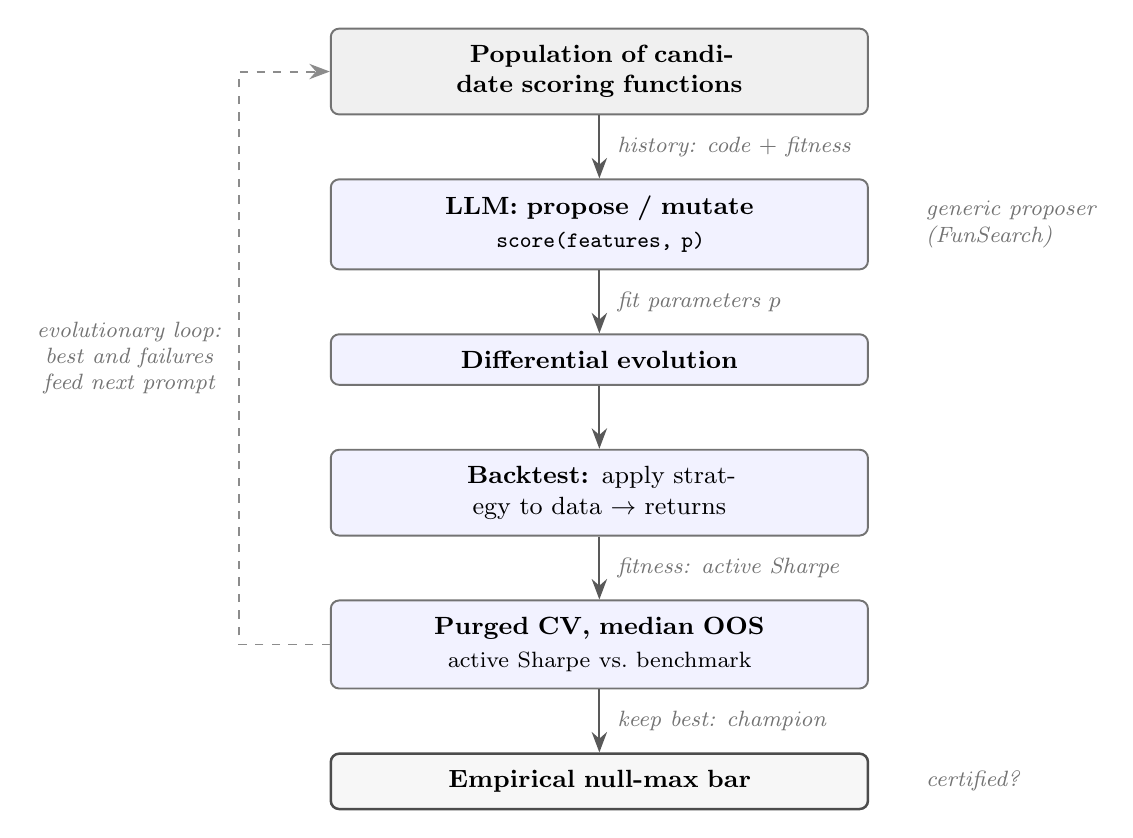
\begin{tikzpicture}[node distance=8mm and 6mm]
  \node[keynode] (pop) {\textbf{Population of candidate scoring functions}};
  \node[proc, below=of pop] (llm)
    {\textbf{LLM: propose / mutate}\\[1pt]{\ttfamily\footnotesize score(features, p)}};
  \node[proc, below=of llm] (de) {\textbf{Differential evolution}};
  \node[proc, below=of de] (bt)
    {\textbf{Backtest:} apply strategy to data $\rightarrow$ returns};
  \node[proc, below=of bt] (cv)
    {\textbf{Purged CV, median OOS}\\[1pt]{\footnotesize active Sharpe vs.\ benchmark}};
  \node[certnode, below=of cv] (bar) {\textbf{Empirical null-max bar}};
  \draw[flow] (pop) -- node[annot, right=1mm] {history: code $+$ fitness} (llm);
  \draw[flow] (llm) -- node[annot, right=1mm] {fit parameters $p$} (de);
  \draw[flow] (de)  -- (bt);
  \draw[flow] (bt)  -- node[annot, right=1mm] {fitness: active Sharpe} (cv);
  \draw[flow] (cv)  -- node[annot, right=1mm] {keep best: champion} (bar);
  \coordinate (l1) at ($(cv.west)+(-1.15,0)$);
  \coordinate (l2) at ($(pop.west)+(-1.15,0)$);
  \draw[fb] (cv.west) -- (l1) -- (l2)
    node[annot, midway, left=1mm, align=center] {evolutionary loop:\\ best and failures\\ feed next prompt} -- (pop.west);
  \node[annot, right=6mm of llm] {generic proposer\\ (FunSearch)};
  \node[annot, right=6mm of bar] {certified?};
\end{tikzpicture}
\caption{The LATSS loop. The LLM proposes and mutates strategy structure from the scored history,
differential evolution fits parameters, and the evaluator scores by cross-validated active Sharpe and
certifies the champion against the null-max bar.}
\label{fig:loop}
\end{figure}

\subsection{Two ways to use the loop}

There are two ways to use LATSS. The first is \emph{generative}: you have a set of candidate indicators
you believe might predict returns, and you run the loop to find a strategy that combines them. The search
will overfit if left unchecked, so you trust the result only if it clears the skill bar, the statistical
test a genuine edge must pass.

The second is \emph{diagnostic}: you are developing a single indicator and want to know whether it
actually carries signal. You give it to the loop mixed in with several pure-noise indicators, without
telling the loop which is which. If the loop repeatedly singles out your indicator and its strategy clears
the bar, run after run, that is evidence the indicator is real rather than a lucky fit.

Both uses rely on the same thing: the loop must reject noise and recover a genuine signal once it is
strong enough. That is the property the rest of the paper tests.

\subsection{Language model versus genetic search as the proposer}
\label{sec:whyllm}

The proposal step of the loop does not require a language model. A classical genetic or random search
fills the same role: fix a grammar of expressions over the features, meaning a list of allowed
operations such as addition, multiplication, and a few transforms, together with a maximum formula
size, and generate or mutate formulas mechanically. Section~\ref{sec:method} builds exactly such
searchers; they cost milliseconds per candidate instead of a model call, and they carry most of the
statistics in this paper. The use of a language model therefore needs a justification. Two
properties argue for it, and one open question decides whether they matter in practice;
Table~\ref{tab:whyllm} summarizes the reasons and what this paper can say about each.

\begin{table}[htbp]
\centering
\caption{Reasons for using a language model as the proposer, and the status of each in this paper.}
\label{tab:whyllm}
\small
\begin{tabular}{p{3.4cm} p{5.3cm} p{5.3cm}}
\toprule
Reason & What it buys & Status \\
\midrule
Open representation & Any short Python function is reachable; no grammar must be designed, and forms
the designer did not anticipate cost nothing & Structural property; demonstrated for program search in
general by FunSearch~\cite{funsearch}, not separately measured here \\
\addlinespace
Semantic prior & On features with meaningful names, proposals cluster around economically plausible
combinations, and the model can rank hypotheses so that fewer need testing
(Section~\ref{sec:prior}) & Untested here: the test-bed's features are opaque by
design, so the prior is inert; the deciding experiment is future work (Section~\ref{sec:future}) \\
\addlinespace
Readable candidates & Each champion is commented code a practitioner can audit, not an expression
tree & Holds by construction \\
\addlinespace
Steering in English & The search is redirected by editing the prompt, not by rewriting a
generator & Holds by construction \\
\addlinespace
Detection power on opaque features & None expected, since the prior has nothing to read & Observed:
champion scores in the same range as mechanical search (E7, Section~\ref{sec:e7}); three runs per
point, not certified \\
\bottomrule
\end{tabular}
\end{table}

The first property, coverage of the space without a hand-designed grammar, is compared concretely in
Section~\ref{sec:generation}.

The second property is that the model's proposal distribution is a prior rather than a blind draw. A
mechanical searcher samples its grammar uniformly; every well-formed formula of a given size is as
likely as any other, including the economically absurd ones. The model samples from its training
distribution, which concentrates probability on code resembling what people have written about the
problem. When the features carry meaningful names, such as momentum, book-to-price, or realized
volatility, the model's proposals cluster around combinations that published economic reasoning
considers plausible, so the search may reach a good candidate in far fewer evaluations than blind
search needs. This prior is the only channel through which a language model can add detection power
over a mechanical search of the same vocabulary; representation aside, everything else the model does,
a mechanical searcher does for free.

The measured results of this paper bound the second property rather than confirm it. The synthetic
test-bed strips the feature names deliberately, because controlling the signal strength requires
features with no meaning, so the prior has nothing to act on there. E7 (Section~\ref{sec:e7}) shows
the consequence: with opaque features, the language model's champions scored in the same range as those
of mechanical search. The prior also has a known cost in this domain, discussed in
Section~\ref{sec:looptoinvention}: the ideas most represented in training are the published ones, and
in trading a published signal is a crowded one.

The certification machinery of Section~\ref{sec:method} works identically for any proposer, so the
empirical contribution of the paper does not depend on whether the model's prior helps. The language
model is kept for its open representation and for readability, since each champion is commented code a
practitioner can audit. Whether its prior buys detection power on nameable features is the open
question; the experiment that would decide it is stated in Section~\ref{sec:future}. If the prior buys
nothing there, the language model is a convenience of representation and the loop is a genetic search
with a well-calibrated test.

\subsection{Construction and cost of the two generators}
\label{sec:generation}

The previous subsection gave the arguments; this one compares the two generators as working machinery,
because the difference is concrete. Every search needs a component that produces the next candidate
scoring function, and the two paths build that component in entirely different ways.

\paragraph{Generation with the language model.} The generator is a prompt. The loop assembles the
scored history, the source code of previously tried scoring functions together with their
cross-validated scores, strongest first, and sends it to the model with a fixed task description. The
model returns the Python source of one new scoring function. No part of the space of possible
strategies is written down anywhere: the model may emit any function of the features that is valid
Python, including conditionals, intermediate quantities, and compositions nobody specified. The
engineering burden sits elsewhere. The emitted code is untrusted text, so the loop must parse it,
reject code that does not compile or that references anything outside the allowed inputs, execute it in
a restricted environment, and handle the fraction of proposals that fail these checks. The harness used
here checks compilation but does not enforce the input restriction, and one champion in E7 read the raw
price series, which the prompt forbids (Section~\ref{sec:e7}). Steering the
generator is done in English: adding a feature means naming it in the prompt, and biasing the search
toward or away from a style of rule means editing a sentence.

\paragraph{Generation without the language model.} The generator must be coded by hand, and coding it
means writing down, in advance, every form a candidate may take. For the nonlinear searcher of this
paper that meant choosing the full inventory explicitly: the four features as leaves; five unary
operations (negation, absolute value, sign, clipping, and standardization of a stock's feature
against its own recent history); seven binary
operations (addition, subtraction, multiplication, a division protected against zero denominators,
maximum, minimum, and a threshold gate); a maximum expression depth of three; and numeric constants
drawn at random and fixed into the expression. On top of the inventory sit two routines: one that
samples a random expression tree from these pieces, and one that compiles a tree into an executable
scoring function. The whole generator is a few hundred lines, written once. Its candidates are valid by
construction, so no parsing or sandboxing is needed, and each one costs a few milliseconds to
generate and evaluate. The linear searcher is simpler still: the form is fixed as one weight per
feature, and generation is nothing more than letting the optimizer move the four weights.

\paragraph{The comparison.} Each path is better at what the other is worst at.

\begin{itemize}[leftmargin=1.4em]
\item \emph{Coverage of the space.} The hand-coded grammar reaches exactly what its inventory implies
and nothing else; any operation the designer did not anticipate is unreachable at any budget. The model
reaches any short program, including conditionals and intermediate quantities no grammar was written to
produce, as in FunSearch~\cite{funsearch}, where variation happens in an open programming language. This
is the language model's structural advantage in generation.
\item \emph{Cost.} A mechanical candidate costs milliseconds and no tokens; a model-generated candidate
costs a network call, seconds of latency, and metered tokens, a difference of several orders of
magnitude per candidate. This is why the statistics of this paper come from the mechanical searchers, 10 to
10{,}000 candidates per run across hundreds of runs, while the language-model arm has nine runs.
\item \emph{Cost of the bar.} Certification requires rerunning the full search on roughly one hundred
scrambled datasets (Section~\ref{sec:bar}), so the bar costs one hundred searches, whatever one search
costs. For the mechanical searcher that is minutes; for the model-driven searcher it is one hundred
times the token cost of the original run. The open representation that is the model's advantage in
coverage directly inflates the price of certifying what it finds.
\item \emph{Validity and audit of the class.} The grammar states the strategy class exactly, which
makes the same-class condition easy to satisfy and easy to verify. The model's class is implicit,
namely whatever it tends to emit under the prompt, so the only way to characterize it is empirically,
by running it.
\item \emph{Quality of the draw.} The grammar samples blindly; the model samples from a prior
(Section~\ref{sec:whyllm}). On nameless features the prior is inert, and in E7 the model's champions scored in the same range as
mechanical search. On nameable
features the prior is the model's one potential advantage in proposal quality, and it is unmeasured.
\end{itemize}

On every axis measured in this paper, cost, statistics, and ease of certification, the hand-coded
generator wins, and nothing in our results justifies the model's price on an opaque vocabulary. The
axes on which the model wins, coverage without design and a prior that can read feature names, are
respectively unpriced and unmeasured here, and they are the reason the model stays in the loop as the
default proposer for real feature sets, where the vocabulary is nameable and the space of sensible
rules is not known in advance.

\section{Validation methodology}
\label{sec:method}

A search cannot be validated by the scores it assigns itself, so we test the
loop on problems where the right answer is known in advance. We build a synthetic test-bed from real
market data in which we control exactly how much real
signal exists, from none at all to plenty, by planting it ourselves. We then run the loop many times over
and ask three questions. When there is nothing to find, does it correctly find nothing, or does it hand
us a strategy anyway? When there is something to find, does it find it? And how strong does the signal
have to be before it does?

Answering these takes two pieces of machinery beyond the loop itself. The first is a way of scoring
candidates that cannot leak future information into the past, which is the cross-validation. The second
is a way of knowing how good a score luck alone can produce, which is the skill bar, and it is needed
because a search that tries thousands of candidates will always find something that looks good; the
question is never whether the best candidate looks good but whether it looks better than the best
accident. Everything in this section is one of those pieces: the market we test on, the planted signal,
the scoring, the searchers that let us repeat the experiment at scale, and the bar.

\paragraph{Test-bed.} The universe is the seven ``Magnificent-7'' US equities (AAPL, MSFT, GOOGL,
AMZN, NVDA, META, TSLA), daily from January 2015 to September 2026 (2{,}952 trading days, about 11.7 years, for E1, E3, and E5;
E4, E7, and E12a used the same panel extended by one day, 2{,}953 trading days). The universe is
fixed in advance and the predictive features are synthetic, so survivorship and universe-selection
effects do not enter these experiments. Each bar the strategy holds the single highest-scoring name,
and the benchmark is the equal-weight portfolio. The
metric throughout is the \emph{active Sharpe}. Let $r^{\mathrm{strat}}_t$ be the strategy's net daily
return (the return of the name it holds on day $t$, after costs) and $r^{\mathrm{bench}}_t$ the net daily
return of the equal-weight portfolio of the seven names. The active return is their difference,
$a_t = r^{\mathrm{strat}}_t - r^{\mathrm{bench}}_t$, and the active Sharpe is its annualized
mean-over-standard-deviation,
\begin{equation}
\mathrm{active\ Sharpe} \;=\; \frac{\overline{a}}{\mathrm{sd}(a)}\,\sqrt{P},
\qquad P = 252\ \text{trading days per year},
\label{eq:activesharpe}
\end{equation}
where $\overline{a}$ and $\mathrm{sd}(a)$ are the sample mean and standard deviation of the daily active
returns. Subtracting the benchmark isolates selection skill: holding the benchmark gives $a_t=0$ and an
active Sharpe of zero. A single name inherits the basket's bull-market trend, so its standalone Sharpe
would credit that trend rather than the skill of picking it.

\paragraph{Synthetic features.} A feature here is an input signal, one number per name per day, that the
scoring function reads; it is the raw material a strategy is built from, in the way a momentum or
volatility measure would be. It is not itself a strategy or a function. Instead of real indicators we
supply synthetic signals whose predictive content we set exactly, so signal and noise are known ground
truth. Each name is given four such signals, \code{feat\_a} through \code{feat\_d}. In the negative
control all four are persistent, unit-variance noise: each day's value is $0.9$ times the previous day's
plus a fresh random shock (a first-order autoregressive process, AR(1), with coefficient $\phi=0.9$), so
the series drifts slowly and looks like a plausible indicator rather than day-to-day random noise, which
makes it harder for the bar to reject. In the positive control one
hidden slot (\code{feat\_c}) carries a cross-sectional predictor: for every name $n$ and day $t$,
\begin{equation}
\code{feat\_c}[n,t] \;=\; \rho \, z[n,t] \;+\; \sqrt{1-\rho^{2}}\;\varepsilon[n,t],
\label{eq:synth}
\end{equation}
where $z[n,t]$ is the signal, a standardized view of the name's future return, and $\varepsilon$ is
unit-variance noise of the same persistent AR(1) kind as the other features, independent of $z$. The intuition is a single dial $\rho\in[0,1]$ that mixes signal and
noise. Because $z$ and $\varepsilon$ are both unit-variance and independent, the weights $\rho$ and
$\sqrt{1-\rho^{2}}$ are exactly the ones that keep the total variance equal to one for every $\rho$
($\rho^{2}+(1-\rho^{2})=1$). This is not vol normalization; it means turning the dial changes only how
much of the feature is signal, not its scale. At $\rho=0$ the feature is pure noise, at $\rho=1$ it is
the pure predictor, $\rho^{2}$ is the fraction of its variance that is signal (equivalently $\rho$ is its
correlation with $z$), and the constant scale matters because it stops the searcher from detecting signal
from the feature's magnitude: only its relationship to returns changes (Figure~\ref{fig:dial}).
Concretely, the signal $z$ is
built in two steps. First, $\mathrm{ex}[n,t]$ (short for excess return) is how much name $n$ beats the
universe over the next 21 trading days: its raw forward return $\mathrm{price}[n,t{+}21]/\mathrm{price}[n,t]-1$ minus the
average forward return across the seven names on day $t$. Second, $z[n,t]$ standardizes this per name,
subtracting $\mathrm{ex}$'s mean and dividing by its standard deviation (computed over the full sample),
so $z$ is unit-variance. The searcher is told none of this.
\code{feat\_c} is a deliberate synthetic oracle built from future returns, used to set a known signal
strength; it is the predictor under test rather than a tradable feature, and is the only route by
which forward information enters the experiment. One subtlety: the standardization of $z$ divides by the
mean and standard deviation of $\mathrm{ex}$ computed over the whole sample, which uses data a live
strategy could not see. In a real predictor that would be a look-ahead error. It is harmless here because
$z$ is not something anyone trades; it is the known signal we inject, and the whole-sample
standardization only calibrates how strong the injected signal is. It changes nothing about how a
strategy is backtested.

\begin{figure}[htbp]
\centering
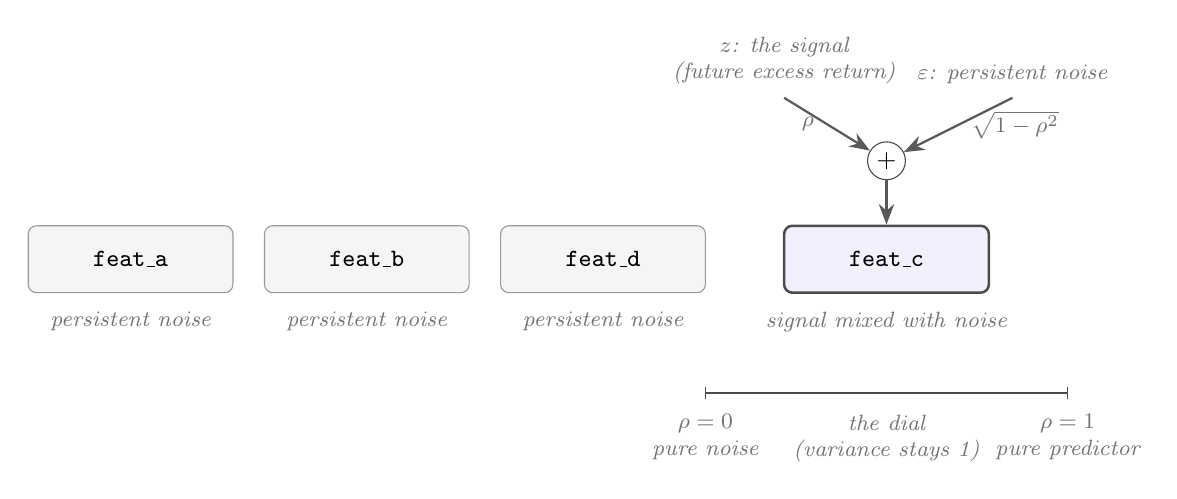
\begin{tikzpicture}[font=\small]
  \foreach \x/\nm in {0/{feat\_a}, 3/{feat\_b}, 6/{feat\_d}} {
    \node[rectangle, rounded corners=3pt, draw=black!40, fill=black!4,
          minimum width=2.6cm, minimum height=0.85cm] at (\x,0) {\ttfamily\nm};
    \node[annot, anchor=north, align=center] at (\x,-0.55) {persistent noise};
  }
  \node[rectangle, rounded corners=3pt, draw=black!70, line width=0.9pt, fill=blue!6,
        minimum width=2.6cm, minimum height=0.85cm] (fc) at (9.6,0) {\ttfamily feat\_c};
  \node[annot, anchor=north, align=center] at (9.6,-0.55) {signal mixed with noise};
  \node[annot, anchor=south, align=center] (z) at (8.3,2.1) {$z$: the signal\\ (future excess return)};
  \node[annot, anchor=south, align=center] (e) at (11.2,2.1) {$\varepsilon$: persistent noise};
  \node[circle, draw=black!70, inner sep=1.5pt] (plus) at (9.6,1.25) {$+$};
  \draw[flow] (8.3,2.05) -- node[annot, left=1pt] {$\rho$} (plus);
  \draw[flow] (11.2,2.05) -- node[annot, right=1pt] {$\sqrt{1-\rho^{2}}$} (plus);
  \draw[flow] (plus) -- (fc);
  \draw[black!70, line width=0.8pt] (7.3,-1.7) -- (11.9,-1.7);
  \foreach \x in {7.3, 11.9} \draw[black!70] (\x,-1.78) -- (\x,-1.62);
  \node[annot, anchor=north, align=center] at (7.3,-1.85) {$\rho=0$\\ pure noise};
  \node[annot, anchor=north, align=center] at (11.9,-1.85) {$\rho=1$\\ pure predictor};
  \node[annot, anchor=north, align=center] at (9.6,-1.85) {the dial\\ (variance stays 1)};
\end{tikzpicture}
\caption{The four input features of the test-bed. Three are persistent noise. The fourth,
\code{feat\_c}, mixes a known signal $z$ with persistent noise through the dial $\rho$ of
Eq.~\eqref{eq:synth}: at $\rho=0$ it is pure noise, at $\rho=1$ the pure predictor, and its scale is the
same at every setting, so only its signal content changes.}
\label{fig:dial}
\end{figure}

\paragraph{Cross-validation.} We use purged, embargoed, chronological six-fold cross-validation~\cite{deprado}. The
pool is cut into six contiguous blocks (Figure~\ref{fig:cv}); each serves once as the test fold, and training is every
other bar except an embargo band of 250 trading days on each side of the test block. The embargo
exceeds the longest lookback the mechanical searchers use (119 days), so for them no training bar shares
a lookback window with a test bar. Code written by the language model is not restricted in this way; one
E7 champion used a lookback of 285 days (Section~\ref{sec:e7}). We
avoid the common alternative of random 75/25 quarter splits, in which adjacent quarters overlap
through warm-up and the split is not chronological. A permissive scheme is doubly damaging, because
fitness and the noise bar are computed under the same cross-validation, so leakage inflates a
signal's score and lowers the bar at the same time.

\begin{figure}[htbp]
\centering
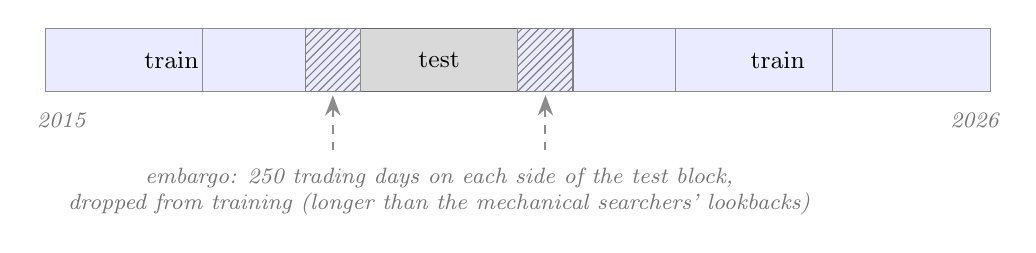
\begin{tikzpicture}[font=\small]
  \draw[draw=black!45, fill=blue!8] (0,0) rectangle (12,0.8);
  \draw[draw=black!60, fill=black!15] (4,0) rectangle (6,0.8);
  \draw[draw=black!50, pattern=north east lines, pattern color=black!50] (3.3,0) rectangle (4,0.8);
  \draw[draw=black!50, pattern=north east lines, pattern color=black!50] (6,0) rectangle (6.7,0.8);
  \foreach \x in {2,4,6,8,10} \draw[black!45] (\x,0) -- (\x,0.8);
  \node at (5,0.4) {test};
  \node at (1.6,0.4) {train};
  \node at (9.3,0.4) {train};
  \node[annot, anchor=north] at (0.2,-0.15) {2015};
  \node[annot, anchor=north] at (11.8,-0.15) {2026};
  \draw[fb] (3.65,-0.75) -- (3.65,-0.05);
  \draw[fb] (6.35,-0.75) -- (6.35,-0.05);
  \node[annot, anchor=north, align=center] at (5,-0.85)
    {embargo: 250 trading days on each side of the test block,\\ dropped from training (longer than the mechanical searchers' lookbacks)};
\end{tikzpicture}
\caption{The purged, embargoed cross-validation. The eleven years are cut into six blocks and each block
takes one turn as the test set, with the rest used for training except an embargo band on each side of
the test block, dropped so that no lookback window spans both training and testing. The figure shows one
of the six folds.}
\label{fig:cv}
\end{figure}

\paragraph{Searchers.} The LLM proposes structures as described in Section~\ref{sec:impl}. Measuring the
loop statistically means running it hundreds to thousands of times, which is too slow and costly with
LLM calls, so in place of the model we also use three mechanical searchers that plug into the same
scoring contract and evaluation stack. Each one proposes scoring rules from a different family (a
strategy \emph{class}, the term used below), and the families differ in how flexible a rule they allow.
The \emph{linear} searcher proposes only weighted sums of the four features,
$w_a\,\code{feat\_a}+w_b\,\code{feat\_b}+w_c\,\code{feat\_c}+w_d\,\code{feat\_d}$, with the four weights
fit by the numerical optimizer; these are the simplest rules available. The \emph{nonlinear} searcher
generates random formulas that combine the features more freely, multiplying them, clipping them, or
switching one on and off depending on another; each formula's constants are set when it is generated, so
no fitting is needed and trying ten thousand candidates is cheap. A third searcher, which evolves such
formulas by mutation and selection (ordinary genetic programming), is implemented in the released code
but was not used in the experiments reported here. The nonlinear family matters most for the skill
bar: because it can express far more shapes of rule, it is also far better at fitting pure noise, so it
is the hardest test of whether the bar holds. It stands in for an LLM writing arbitrary code, but only as
a stand-in, since its formulas are drawn from a fixed menu of operations while arbitrary code has no such
limit (Eq.~\eqref{eq:vc} returns to this).

\paragraph{Search capacity, evaluation capacity, and search budget.} Three different things are easy to conflate here, so we give
each a name. \emph{Search capacity} is how flexible the family of rules is, how many different shapes of
rule it can express at all; the linear family above is small in this sense, the nonlinear family large.
\emph{Evaluation capacity} is how much tuning happens inside each single candidate when the optimizer
fits its parameters to the data. \emph{Search budget} is simply how many candidates the search tries.
All three are routes to fitting noise, and they need not move together. The nonlinear mechanical searcher
has a fixed search capacity and a dial for its budget, while an LLM writing arbitrary code has an
effectively unlimited search capacity. The experiment in Section~\ref{sec:e4} turns the budget dial
alone and holds everything else still.

\subsection{The null-max skill bar}
\label{sec:bar}

Under a sufficiently expressive, persistent search no partition of the data is truly out of sample
(Section~\ref{sec:whybar}), so we do not certify against a hold-out. We certify in sample against a
null-max bar~\cite{nullmax}, the highest cross-validated active Sharpe the strategy class reaches on
data whose signal has been destroyed. A champion that cannot beat what its own class extracts from
noise has no measured skill.

\paragraph{A VC-inspired capacity scale.} The VC dimension of a family of rules, written $h$, is a
standard measure of its flexibility~\cite{vapnik}: roughly, the largest number of data points the family
can fit in every possible configuration. A more flexible family has a larger $h$, and with it a greater
ability to manufacture apparent skill from noise. For a family of VC dimension $h$ evaluated over $m$
trading sessions spanning $Y$ years, luck alone produces an annualized Sharpe of order
\begin{equation}
\mathrm{bar}_{\mathrm{VC}} \;\approx\; \sqrt{\tfrac{2\,h\,\log(e\,m/h)}{Y}} .
\label{eq:vc}
\end{equation}
This is heuristic dimensional analysis, a VC-inspired capacity scale rather than a bound on Sharpe
derived for our exact procedure: the constant does not account for the step that selects the single best candidate or the
dependence across observations. As an order of magnitude, a linear combination of the four features
($h\approx 5$) sits near 2.5 at our sample size, while an unconstrained code-writing class has
effectively unbounded $h$ and no finite scale.

\paragraph{Empirical bar (null-max, operative).} The VC scale is adversarial, a ceiling rather than a
working hurdle. The operative bar is measured on the data itself, using what we call a \emph{scramble}: a
copy of the return data in which the signal has been deliberately destroyed but everything else is left
in place. One scramble is produced and used as follows.
\begin{enumerate}[leftmargin=1.6em]
\item For every name $n$ and every day $t$, flip an independent fair coin
$\sigma[n,t]\in\{-1,+1\}$ and set the scrambled return to $\tilde r[n,t]=\sigma[n,t]\,r[n,t]$. Each daily
return keeps its magnitude and randomly keeps or reverses its direction, so any relation between the
features and the returns is destroyed while the size and texture of the returns are preserved. (The sign
flip is a Rademacher-style randomization.)
\item Recompute the equal-weight benchmark from the scrambled returns.
\item Run the identical search on the scrambled data: same family of rules, same search budget, same
parameter fitting, same cross-validation, features untouched.
\item Record the best cross-validated active Sharpe that search finds, the most skill it could fake on
data containing none.
\end{enumerate}
Repeating this for many independent scrambles, one hundred to one thousand in our experiments, gives a
distribution of best-on-noise scores. The bar is its 95th percentile, written $\mathrm{bar}_q$
(Figure~\ref{fig:nullmax}). The VC expression is a conservative capacity-based reference scale; the
empirical null-max bar is the operative calibration.

\begin{figure}[htbp]
\centering
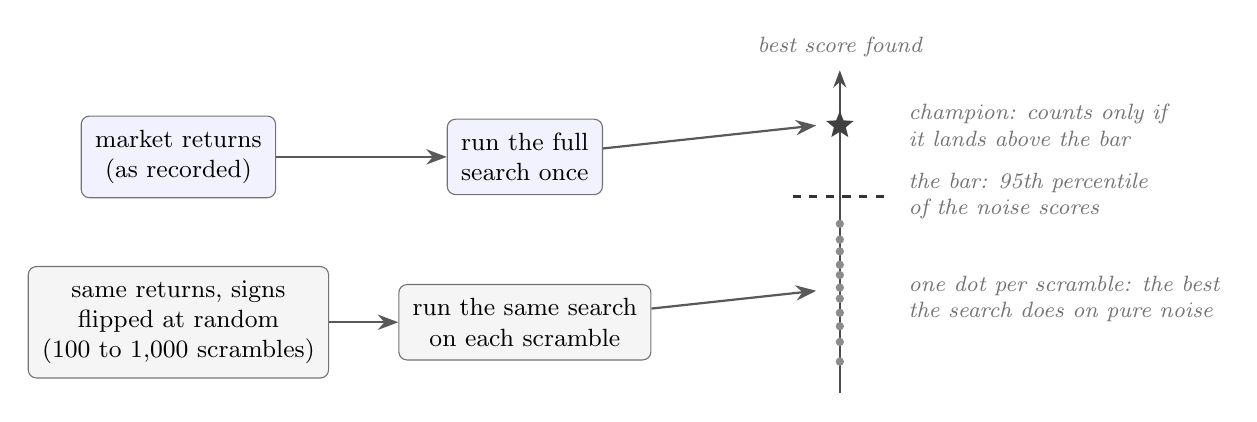
\begin{tikzpicture}[font=\small]
  \node[rectangle, rounded corners=3pt, draw=black!55, fill=blue!5, align=center, inner sep=5pt]
    (r1) at (0,2.1) {market returns\\ (as recorded)};
  \node[rectangle, rounded corners=3pt, draw=black!55, fill=blue!5, align=center, inner sep=5pt]
    (r2) at (4.4,2.1) {run the full\\ search once};
  \node[rectangle, rounded corners=3pt, draw=black!55, fill=black!4, align=center, inner sep=5pt]
    (n1) at (0,0) {same returns, signs\\ flipped at random\\ (100 to 1{,}000 scrambles)};
  \node[rectangle, rounded corners=3pt, draw=black!55, fill=black!4, align=center, inner sep=5pt]
    (n2) at (4.4,0) {run the same search\\ on each scramble};
  \draw[flow] (r1) -- (r2);
  \draw[flow] (n1) -- (n2);
  \draw[black!70, line width=0.8pt, -{Stealth[length=2.2mm]}] (8.4,-0.9) -- (8.4,3.2);
  \node[annot, anchor=south] at (8.4,3.25) {best score found};
  \foreach \y in {-0.5,-0.25,-0.05,0.12,0.3,0.44,0.6,0.73,0.9,1.05,1.25}
    \fill[black!45] (8.4,\y) circle (1.5pt);
  \draw[dashed, black!80, line width=0.9pt] (7.8,1.6) -- (9.0,1.6);
  \node[annot, anchor=west] at (9.15,1.6) {the bar: 95th percentile\\ of the noise scores};
  \node[star, star points=5, star point ratio=2.3, fill=black!75, inner sep=1.6pt] at (8.4,2.5) {};
  \node[annot, anchor=west] at (9.15,2.5) {champion: counts only if\\ it lands above the bar};
  \node[annot, anchor=west] at (9.15,0.3) {one dot per scramble: the best\\ the search does on pure noise};
  \draw[flow] (r2) -- (8.1,2.5);
  \draw[flow] (n2) -- (8.1,0.4);
\end{tikzpicture}
\caption{How the null-max bar is built. The same search runs once on the real returns, giving the
champion, and once on each of 100 to 1{,}000 copies whose signs are flipped at random, which removes any
relation between features and returns. Each scrambled run records the best score the search finds
on pure noise; the 95th percentile of those scores is the bar, and the champion is credited with
skill only if it beats it.}
\label{fig:nullmax}
\end{figure}

\paragraph{Same-class condition and certification.} What must match is the search procedure itself.
The bar is built by running a search on scrambled data, and the champion is produced by running a
search on the real data; the two searches must be the same procedure in every respect, with the data as
the only difference. The same respects are: the family of rules the search may emit (linear weights
versus unrestricted expression trees), the search budget (how many candidates are tried), the parameter
fitting applied to each candidate, and the cross-validated score used to rank them. We call a bar
\emph{matched} when all of these agree with the search that produced the champion, and \emph{mismatched}
when any of them differs in a way that changes how well the search fits noise. A matched bar answers the
right question, namely what score this exact search achieves when there is nothing to find. A mismatched
bar answers that question for some other search: computed over a smaller class, or with a smaller
budget, it underestimates the achievable noise fit and admits overfits, which
Section~\ref{sec:ablation} measures. A consequence of the condition is that the bar is not reusable.
Any change to the search, a new feature, a larger rule family, a higher budget, or a different fitting
procedure, invalidates the previously computed bar, and a new bar must be computed by running the
modified search on the scrambled data again. This recomputation is the recurring cost of the method.
When the cost is paid the guarantee held in our tests: Section~\ref{sec:e4} measures a false-positive
count of 0 of 30, on one data realization, at every budget from ten to ten thousand candidates, each budget judged against its own
recomputed bar. A champion is null-certified (it passes the null-max test) when its cross-validated
active Sharpe exceeds $\mathrm{bar}_q$, where $q=0.95$. The VC scale is reported as a ceiling and is never used as the
gate. Null certification means only that the observed champion exceeds the empirical 95th-percentile
null maximum under the stated class, search procedure, and null construction. It is not a guarantee of
future profitability.

\subsection{Null construction and its assumptions}
\label{sec:nullassume}

The sign flip multiplies each entry of the return matrix by an independent $\pm 1$. This removes the
feature-to-return relation, and with it the temporal dependence, the cross-sectional and common-factor
structure, and the volatility-state relationships present in the real panel. The bar is therefore the
best in-class fit under a null in which returns are independently sign-randomized conditional on their
magnitudes. It is a calibrated null reference for this selector under a directional-exchangeability
assumption: absent a feature-to-return relation, the sign of each name's return is exchangeable at the
resolution the selector acts on, and the long-only top-one selection earns the held name's return, whose
sign the flip removes. The bar's operating characteristics under richer dependence structures are not
established here. Nulls that preserve more structure, a by-day sign flip, a cross-sectional permutation of
returns across names, and block or stationary bootstraps, would test robustness to that assumption,
and we leave them to future work.

\subsection{Alternatives to the null-max bar}
\label{sec:whybar}

The standard alternatives are each unsuited to this setting. The Deflated Sharpe
Ratio~\cite{deflated} deflates by a trial count, but for an automated search the trial count is
ill-defined, since the search effectively covers the whole class, and it is gameable because fewer
trials incur a smaller penalty. The invariant that matters is the class's capacity, which the
null-max bar measures. Permutation and shift-the-signal tests select by a uniform maximum over
sampled configurations, while the fitness selects by differential evolution, which fits noise more
thoroughly, so they under-price the overfitting that produced the champion; we keep shift-the-signal only
as a reported diagnostic. A hold-out is not automatically sufficient when it becomes part of an
iterative research loop: with an expressive class and repeated adaptive re-use of the reserved period
across attempts, the hold-out is fit too. A genuinely untouched hold-out, used once at the end, does
give protection; the concern here is the iterative case.

\section{Experimental design}
\label{sec:design}

Each experiment answers one of the laboratory questions of Section~\ref{sec:method}. This section
specifies the experiments; Section~\ref{sec:results} reports the results. Throughout, the injected
predictor \code{feat\_c} literally contains future returns (Eq.~\eqref{eq:synth}): it is a calibrated
oracle used solely to place a known amount of signal on a controlled scale, not a tradable or
economically causal feature and not a simulated look-ahead backtest, and no part of the search or the
bar sees its construction. The experiments measure signal recovery, not a trading result. All runs use
purged, embargoed cross-validation and the empirical null-max bar; ``clears'' means the champion's
cross-validated active Sharpe exceeds the bar; mechanical conditions use 30 runs and the LLM condition
3 runs per point. Experiment labels follow an earlier plan, and planned experiments that were not run are
not reported, which is why some numbers are absent. The scripts producing every table are in the repository (\code{exp\_v2\_synth.py},
with \code{--bmax 10000 --n-pools 30} for E4, and \code{exp\_v2\_fixes.py}).

\subsection{E3: estimation of the null-max bar}

We need the numerical value of the bar before any
other test can be read. To obtain it, we take the real returns and remove their signal with the sign-flip
scramble of Section~\ref{sec:bar}: every daily return keeps its size, and its direction is set by an
independent coin flip, so no feature can predict the result. We then run the identical strategy search on
the scrambled data and record the best cross-validated score it finds. Any score earned on this data is
overfitting by definition, because there is nothing real to find. We repeat this up to one thousand
times, each time with a fresh scramble, and collect the best scores into a distribution. The bar is the
95th percentile of that distribution. The experiment also measures how many scrambles are needed before
that percentile settles to a stable value, which fixes how many repetitions the later experiments use.

\paragraph{Inputs.} The Magnificent-7 daily panel of Section~\ref{sec:method} (2{,}952 trading days),
the all-noise feature set (four persistent noise series per name, no planted signal), and the two
searcher families of Section~\ref{sec:method}: the nonlinear family of random formulas and the linear
family of weighted sums.

\paragraph{Procedure.} For each of 1{,}000 repetitions: (1) draw an independent $\pm 1$ coin flip for
every name and every day and multiply each daily return by it; (2) recompute the equal-weight benchmark
from the flipped returns; (3) run the searcher on the flipped data exactly as it would run on real data,
the nonlinear searcher drawing 200 random formulas of depth at most three and the linear searcher fitting
its four weights by differential evolution with a budget of 150 evaluations; (4) score every candidate by
purged cross-validated active Sharpe and record the single best score of the repetition. The procedure is
run separately for the two families, because each must be measured against its own behavior on noise.

\paragraph{Outputs and analysis.} The 1{,}000 recorded best-on-noise scores form the null distribution of
each family. We report its mean and its 95th percentile, which is the bar. To determine how many
repetitions the estimate needs, we also recompute the 95th percentile from the first 30, 50, 100, 250,
and 500 repetitions and compare: the count at which the value stops moving is the repetition count the
later experiments must meet. A family whose bar is still drifting after 1{,}000 repetitions would mean
the later certifications rest on an unstable threshold, which is why this experiment runs first.

\subsection{E1: false-positive rate and detection power}

This is the main test of the loop. We build
the test data so that the right answer is known in advance: the feature \code{feat\_c} is constructed
from the future returns themselves, so it genuinely predicts, and the parameter $\rho$ of
Eq.~\eqref{eq:synth} sets how strongly, from not at all at $\rho=0$ to almost perfectly at $\rho=1$. At
each value of $\rho$ we run the complete search thirty times with different random seeds and count how
often the champion's score exceeds the bar. At $\rho=0$ there is nothing to find, so every run that
exceeds the bar is a false positive, and the count measures the false-positive rate. At higher $\rho$ the
count measures detection: how often the loop finds the planted feature and passes the bar when a real
signal is present. Plotting that frequency against $\rho$ gives the power curve of the loop. The value of
$\rho$ at which the curve rises from near zero to near one is the weakest signal the loop can reliably
certify.

\paragraph{Inputs.} The same panel; feature sets generated at nine signal strengths, $\rho = 0$,
$0.10$, $0.15$, $0.20$, $0.25$, $0.30$, $0.40$, $0.50$, and $0.70$, each with \code{feat\_c} built from
Eq.~\eqref{eq:synth} and the other three features noise; and the two bars measured in E3, $+0.844$ for
the nonlinear family and $+0.408$ for the linear family.

\paragraph{Procedure.} For every combination of signal strength and searcher family we run the complete
search 30 times. The runs differ in the searcher's random seed, which changes the formulas the nonlinear
searcher draws and the optimizer's path for the linear searcher; the feature realization is held fixed
within each signal strength so the runs face the same data. The 30 runs are therefore repeated searches
of one data set, and their counts describe that data set. To obtain a false-positive count over
independent data, we also repeat the $\rho=0$ condition with a new noise realization for each of the 30
runs. Each run returns one champion, the candidate
with the highest purged cross-validated active Sharpe, and that score is recorded. A run counts as a
certification when its champion's score exceeds the bar of its own family.

\paragraph{Outputs and analysis.} For each combination we report the certification frequency out of 30
and the median champion score. The frequency at $\rho=0$ in the repeated-realization condition is the
observed false-positive rate; with 30 independent runs and zero observed false positives, the true rate
is below 9.5\% at 95\% confidence (one-sided Clopper--Pearson bound). The frequencies across $\rho$ form the power curve. From it we read the threshold,
the smallest $\rho$ at which certification becomes reliable, and convert it to units of active Sharpe
using the oracle calibration of E2, so the threshold can be stated as the weakest signal, in Sharpe
units, that the loop reliably certifies.

\subsection{E2: search amplification}

This experiment measures how much the search overstates a real
signal. For each $\rho$ we know the reference score: what a selector would earn if it ranked names by the
planted feature alone and used nothing else. We compare the champion's cross-validated score to that
reference. The champion routinely scores above it. The reason is that the search does not stop at the
planted feature; it also fits the three noise features, and whatever fit it finds in them adds to the
measured score even though it is not real. The size of this gap quantifies the upward bias of any score
produced by a search, and it is the direct reason a champion's score cannot be read at face value and
must instead be compared to the bar.

\paragraph{Inputs.} The per-run champion scores from E1, and for each $\rho$ an oracle reference: the
active Sharpe earned by a selector that each day ranks the seven names by \code{feat\_c} alone and holds
the top name, computed on the full sample and averaged over 30 independent noise realizations. We also
report the value for the single realization E1 searched. The reference
is what the planted feature is worth on its own, with no search involved.

\paragraph{Procedure.} For each $\rho$ the 30 champion scores from E1 are placed next to the oracle
reference and the difference is measured. No new searches are run; this is a re-analysis of the E1 output
that isolates one quantity, the gap between what the search reports and what the planted signal is worth.

\paragraph{Outputs and analysis.} We report the oracle reference and the champion scores side by side
across $\rho$. A positive gap at a given $\rho$ measures how much score the search extracted from the
three noise features on top of the real signal. The conclusion is drawn by comparing three numbers at
each $\rho$: the oracle reference, the champion score, and the bar. Champions exceeding the oracle
reference is expected overfitting; the question the experiment settles is whether the bar accounts for
that excess, so that the certification decision can remain anchored to the bar while the raw score is
treated as biased upward.

\subsection{E5: bar misspecification}

This experiment makes a deliberate error in order to measure its
cost. The correct procedure computes the bar with the same family of rules the search uses. Here the
search uses the flexible nonlinear family, but we compute the bar from the simple linear family instead.
The linear family is worse at fitting noise, so its bar is much lower. We then take the champions the
nonlinear search finds on pure noise, certify them against this too-low bar, and count how many pass.
Comparing that count with the count under the correctly matched bar isolates the false-positive rate
caused purely by the mismatch. The result shows what goes wrong when the statistical test is borrowed
from a weaker search than the one actually run.

\paragraph{Inputs.} Pure-noise feature sets ($\rho=0$) and weak-signal sets ($\rho=0.15$); the nonlinear
searcher with its usual budget of 200 candidates; and both bars from E3, the matched nonlinear bar of
$+0.844$ and the mismatched linear bar of $+0.408$.

\paragraph{Procedure.} The nonlinear search is run 30 times at each $\rho$, exactly as in E1, and each
run's champion is kept. Each champion is then judged twice, once against the matched bar and once against
the mismatched bar. Nothing else differs between the two judgments: the champion, the data, and the score
are identical, and only the threshold changes, so any difference in outcomes is attributable to the
threshold alone.

\paragraph{Outputs and analysis.} For each $\rho$ and each bar we report the number of champions out of
30 that pass. At $\rho=0$ every pass is a false positive, so the difference between the two counts is the
false-positive rate caused purely by the mismatch. The experiment turns the same-class condition of
Section~\ref{sec:bar} into a measured quantity: if the two counts were similar, matching the bar to the
search would be a technicality, and a large difference means the family used to compute the bar is a
correctness requirement of the method, not a preference.

\subsection{E4: search-budget dependence}

This experiment varies one quantity, the number of candidate
strategies the search may try, from ten up to ten thousand, with everything else unchanged. More attempts
on signal-free data produce higher best-on-noise scores, so the bar is recomputed at every budget, and we
measure how fast it rises. At each budget we then repeat the E1 measurements: the false-positive rate on
pure noise and the detection rate at fixed signal strengths. The question is whether a large enough
number of attempts eventually produces noise champions that pass even the recomputed bar. The experiment
answers it over three orders of magnitude of budget.

\paragraph{Inputs.} Pure-noise features and planted-signal features at $\rho=0.15$ and $\rho=0.20$; the
nonlinear family; and budgets $B \in \{10, 30, 100, 300, 1{,}000, 3{,}000, 10{,}000\}$.

\paragraph{Procedure.} Running a separate search at every budget would waste computation, so the design
is cumulative. On the noise side, each of 100 scrambles draws a fresh pool of 10{,}000 random formulas,
evaluates all of them on the scrambled data, and records the running best score after the first 10, 30,
100, and so on up to 10{,}000 candidates; the running best after $B$ candidates is exactly what a search
with budget $B$ would have found. The bar at budget $B$ is the 95th percentile of these running bests
across the 100 scrambles. On the signal side the same cumulative design is applied to 30 independent
pools per $\rho$ on the planted-signal data, giving one champion score at every budget for every pool.

\paragraph{Outputs and analysis.} For each budget we report the recomputed bar, the certification
frequency at $\rho=0$ out of 30 against the budget-matched bar, and the certification frequencies at
$\rho=0.15$ and $\rho=0.20$. Three outcomes are possible, and the data decides among them: the bar rises
with budget and false positives appear anyway, meaning budget defeats the correction; the bar rises and
detection of real signal collapses, meaning budget destroys power; or the bar and the real-signal
champions rise together and both error rates hold, meaning the correction tracks the budget over the
tested range.

\subsection{E7: LLM versus mechanical search}

The experiments above use the mechanical searchers, so
this one checks whether the language model behaves differently. We put the model back into the loop as
the component that writes the candidate strategies and run the search at three signal strengths, three
runs each, and compare the model's champion scores with those of the mechanical searchers at the same
signal strengths. The comparison is of raw scores only. A certification would require a bar computed by
rerunning the language-model search on about one hundred scrambled data sets, at about one hundred times
the token cost of the experiment, which we did not do; by the same-class condition of
Section~\ref{sec:bar}, the nonlinear bar of E3 is not the matched bar for this search. Because model
runs are slow and costly, this arm has far fewer repetitions; the mechanical results carry the
statistics, and this experiment is a consistency check.

\paragraph{Inputs.} Planted-signal features at $\rho \in \{0, 0.15, 0.20\}$, with a feature realization
set by each run's seed; and the language model in place of the mechanical searcher. The model was Claude
Opus, the default model of the Claude Code session in which the runs were made, called as a subagent
through a file handoff; the exact model version was not logged.

\paragraph{Procedure.} Each run executes the full loop of Section~\ref{sec:loop} with the model writing
the candidates: up to 12 proposal rounds, each producing one new scoring function from the task
description and the scored history of earlier candidates (proposals that duplicate an earlier one are
rejected), with differential evolution fitting each candidate's parameters under a budget of 60
evaluations and purged cross-validation scoring it. Three runs with different seeds are executed at each
signal strength.

\paragraph{Outputs and analysis.} For each signal strength we report the three champion scores next
to the median champion score of the mechanical nonlinear search from E1. With three runs per point the
comparison supports only a coarse conclusion. Two features of the design limit what the model can use.
The prompts give it the task description, the four feature names, and the code and scores of earlier
candidates, and no prices or feature values; the subagent ran inside the project directory, however, and
we did not restrict its access to files, so we cannot exclude that it read the code that generates the
features. And the features are opaque series with no meaningful names, so the model's knowledge of
markets gives it no usable advantage here; a test with meaningful features is described in
Section~\ref{sec:future}.
\section{Results}
\label{sec:results}

\subsection{The null-max bar (E3)}
\label{sec:e3}

Over 1000 sign-flip scrambles, the 95th-percentile bar is $+0.844$ for the high-capacity nonlinear
class and $+0.408$ for the bounded linear class. The gap reflects both capacity and search mechanism:
the linear class is fit by continuous differential evolution and the nonlinear class by discrete
enumeration of trees, so the two are not a controlled capacity comparison. The classes also differ in
how fast the estimate settles. The nonlinear bar is stable beyond roughly 100 scrambles; the linear
bar keeps rising as scrambles increase, with a growing tail maximum, so a small scramble count
under-estimates a low-capacity bar. Experiments E1, E5, and E12a use the 1000-scramble bar; the
budget sweep (Section~\ref{sec:e4}) recomputes the bar at 100 scrambles per budget over the
nonlinear class, which the stability result supports for the 200-candidate search on which it was
measured.

\subsection{Power curve and false positives (E1)}
\label{sec:e1}

Table~\ref{tab:power} gives the certification frequency against injected signal, 30 runs per point,
each class certified against its own bar.

\begin{table}[htbp]
\centering
\caption{Certification power curve (30 runs per point, one data realization per $\rho$). ``Oracle''
is the active Sharpe of a selector that holds the name with the highest \code{feat\_c} each day, a
descriptive full-sample quantity used only to calibrate signal strength and never seen by the search or
the certification. The first oracle column averages 30 noise realizations; the second is the
realization E1 searched.}
\label{tab:power}
\small
\begin{tabular}{c c c c c c}
\toprule
$\rho$ & oracle (mean) & oracle (searched) & nonlinear $P(\text{clear})$ & median champ & linear $P(\text{clear})$ \\
\midrule
0.00 & $-0.25$ & $-0.34$ & 0.00 & $+0.44$ & 0.00 \\
0.10 & $+0.32$ & $+0.46$ & 0.03 & $+0.68$ & 0.00 \\
0.15 & $+0.56$ & $+0.63$ & 0.43 & $+0.83$ & 0.10 \\
0.20 & $+0.83$ & $+0.95$ & 1.00 & $+1.10$ & 0.70 \\
0.25 & $+1.06$ & $+1.21$ & 1.00 & $+1.40$ & 0.80 \\
0.30 & $+1.31$ & $+1.57$ & 1.00 & $+1.77$ & 1.00 \\
0.40 & $+1.77$ & $+1.80$ & 1.00 & $+1.96$ & 1.00 \\
0.50 & $+2.14$ & $+2.17$ & 1.00 & $+2.17$ & 1.00 \\
0.70 & $+2.85$ & $+2.88$ & 1.00 & $+2.79$ & 1.00 \\
\bottomrule
\end{tabular}
\end{table}

\begin{figure}[htbp]
\centering
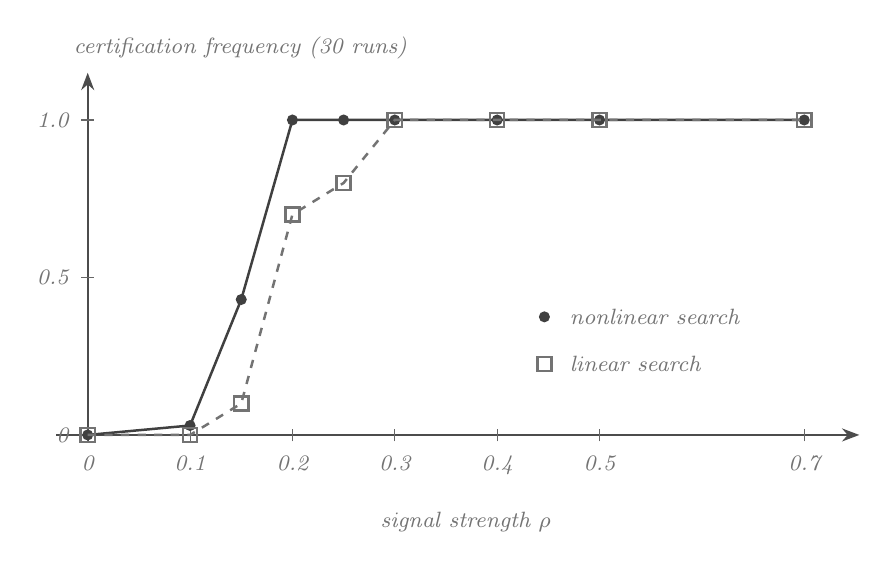
\begin{tikzpicture}[font=\small]
  \draw[black!70, line width=0.8pt, -{Stealth[length=2.2mm]}] (0.8,-0.1) -- (0.8,4.6);
  \draw[black!70, line width=0.8pt, -{Stealth[length=2.2mm]}] (0.4,0) -- (10.6,0);
  \node[annot, anchor=south west] at (0.5,4.65) {certification frequency (30 runs)};
  \node[annot, anchor=north] at (5.6,-0.85) {signal strength $\rho$};
  \foreach \y/\l in {0/0, 2/0.5, 4/1.0} {
    \draw[black!60] (0.72,\y) -- (0.88,\y);
    \node[annot, anchor=east] at (0.68,\y) {\l};
  }
  \foreach \r/\l in {0.8/0, 2.1/0.1, 3.4/0.2, 4.7/0.3, 6.0/0.4, 7.3/0.5, 9.9/0.7} {
    \draw[black!60] (\r,-0.08) -- (\r,0.08);
    \node[annot, anchor=north] at (\r,-0.15) {\l};
  }
  \draw[black!75, line width=0.9pt] (0.8,0) -- (2.1,0.12) -- (2.75,1.72) -- (3.4,4) -- (4.05,4)
    -- (4.7,4) -- (6.0,4) -- (7.3,4) -- (9.9,4);
  \foreach \p in {(0.8,0),(2.1,0.12),(2.75,1.72),(3.4,4),(4.05,4),(4.7,4),(6.0,4),(7.3,4),(9.9,4)}
    \fill[black!75] \p circle (2pt);
  \draw[black!55, dashed, line width=0.9pt] (0.8,0) -- (2.1,0) -- (2.75,0.4) -- (3.4,2.8) -- (4.05,3.2)
    -- (4.7,4) -- (6.0,4) -- (7.3,4) -- (9.9,4);
  \foreach \x/\y in {0.8/0,2.1/0,2.75/0.4,3.4/2.8,4.05/3.2,4.7/4,6.0/4,7.3/4,9.9/4}
    \draw[black!55, line width=0.9pt] (\x-0.09,\y-0.09) rectangle (\x+0.09,\y+0.09);
  \fill[black!75] (6.6,1.5) circle (2pt);
  \node[annot, anchor=west] at (6.8,1.5) {nonlinear search};
  \draw[black!55, line width=0.9pt] (6.51,0.81) rectangle (6.69,0.99);
  \node[annot, anchor=west] at (6.8,0.9) {linear search};
\end{tikzpicture}
\caption{The power curves of Table~\ref{tab:power}. Each point is the fraction of 30 runs whose champion
cleared the family's own bar at that signal strength. The nonlinear search becomes reliable at
$\rho=0.20$ and the linear search at $\rho=0.30$; neither certifies pure noise at $\rho=0$.}
\label{fig:power}
\end{figure}

Figure~\ref{fig:power} plots the two power curves. Certification by the nonlinear search becomes
reliable at $\rho=0.20$, where the oracle active Sharpe is 0.83 on average over noise realizations
(0.95 for the realization searched); at $\rho=0.15$ (oracle 0.56) it occurred in 13 of 30 runs, at
$\rho=0.10$ (oracle 0.32) in 1 of 30, and at $\rho=0$ in none. The linear search becomes reliable at
$\rho=0.30$ (oracle 1.31). The nonlinear search certified at least as often as the linear search at every
signal strength: restricting the class to linear rules lowered the bar but did not lower the detection
threshold here, because the linear champions scored closer to their own bar with more variation from run
to run.

Because these 30 runs share one data realization, their zero count at $\rho=0$ describes that data set.
In the repeated-realization condition, with a new noise realization for every run, the nonlinear search
certified in 0 of 30 runs (median champion $0.40$, maximum $0.74$) and the linear search in 0 of 30
(maximum $0.15$). With 30 independent runs and no false positives, the false-positive rate is below 9.5\%
at 95\% confidence (one-sided Clopper--Pearson).

The oracle at $\rho=0$ is negative ($-0.25\pm0.35$ across realizations) because a selector driven by noise
changes its holding often and pays transaction costs on each change, while the benchmark rebalances
little.

\subsection{Search amplification (E2)}
\label{sec:e2}

The champion's cross-validated score exceeds the oracle reference for the realization searched at
every signal strength up to $\rho=0.40$. At $\rho=0.20$ that reference is 0.95 while the median nonlinear
champion scores 1.10, because the search fits the noise features on top of the real signal; at
$\rho\ge 0.50$ the champion falls to or slightly below the oracle (2.17 against 2.17, and 2.79 against
2.88 at $\rho=0.70$). The amplification is why a
champion's score must be compared with the bar of 0.844 and not read at face value: the champion must beat
what the same search extracts from noise.

\subsection{Same-class ablation (E5)}
\label{sec:ablation}

The certification rule of Section~\ref{sec:bar} requires the bar to be computed by running the same
search that produced the champion. This experiment measures what that requirement is worth by violating
it once, deliberately, and counting the consequences.

The two search families measured in E3 carry different bars on identical data. The nonlinear family can
combine four features through an unrestricted expression tree, so it has many ways to fit noise, and its
best-on-noise score is correspondingly high: its bar is $+0.844$. The linear family, limited to four
weights, has far fewer ways to fit noise: its bar is $+0.408$. Neither number measures signal. Each is
the 95th percentile of the best score that family's search extracts from scrambled, signal-free returns,
so each is the threshold that family must beat before its champion means anything.

Now take the 30 champions the nonlinear search found on pure noise ($\rho=0$). Their median score is
about $+0.44$, which is ordinary noise fitting for this family and sits well below the family's own bar.
Judged against the matched nonlinear bar of $0.844$, 0 of 30 pass. That is the
correct outcome, because there was no signal to find. Judged against the linear bar of $0.408$ instead,
20 of 30 pass. The champions, the data, and the scores are identical in the two judgments; only the
threshold changed. These 30 runs share one data realization, so the count describes that data set; in
the repeated-realization condition of E1, with a new noise realization for every run, 13 of 30 champions
pass the linear bar (95\% interval 26 to 63\%) and none pass their own. Signal-free strategies would be
certified as carrying real signal, because the test asked whether each champion beat what a four-weight linear rule
can extract from noise, while the search that produced the champion was free to build arbitrary
nonlinear expressions and therefore extracts far more from noise than a linear rule does. At the weak signal
strength $\rho=0.15$, the same comparison gives 13 of 30 certifications against the matched bar and 30
of 30 against the mismatched one, so the mismatched bar also makes a weak signal look reliably
detected.

This error is easy to commit in practice. The bar might be estimated with a cheap, simple search to save
computation while the production search is more flexible; the search might be upgraded later, with more
operators or more features, without recomputing the bar; or a threshold might be borrowed from a
published study whose search differed from one's own. In each case the certified output contains noise
champions at whatever rate the capacity gap produces, 13 to 20 of 30 here for a single step down in
capacity on this test-bed.

The direction of the mismatch determines the kind of failure. A bar computed over a class larger than
the search is too high, which costs detection power but keeps the false-positive guarantee. A bar
computed over a class smaller than the search is too low, and the guarantee is gone. The same-class
condition is therefore a correctness requirement of the method, not a preference.

\subsection{Search budget (E4)}
\label{sec:e4}

We hold the class fixed and vary its search budget $B$, recomputing the noise bar (100 scrambles per
budget) and the certification rate at each budget (Table~\ref{tab:capacity}).

\begin{table}[htbp]
\centering
\caption{Budget sweep for the nonlinear class, 30 pools per point. The noise bar rises with budget,
while the certification frequency on noise ($\rho=0$) stays at 0 of 30 up to ten thousand candidates
(one data realization).}
\label{tab:capacity}
\small
\begin{tabular}{c c c c c}
\toprule
budget $B$ & noise bar $q_{95}$ & $P(\text{clear})\,\rho{=}0$ & $P(\text{clear})\,\rho{=}0.15$ & $P(\text{clear})\,\rho{=}0.20$ \\
\midrule
$10$     & 0.59 & 0.00 & 0.77 & 0.77 \\
$30$     & 0.70 & 0.00 & 0.17 & 1.00 \\
$100$    & 0.79 & 0.00 & 0.47 & 1.00 \\
$300$    & 0.88 & 0.00 & 0.37 & 1.00 \\
$1000$   & 0.95 & 0.00 & 0.53 & 1.00 \\
$3000$   & 1.04 & 0.00 & 0.53 & 1.00 \\
$10000$  & 1.20 & 0.00 & 0.37 & 0.97 \\
\bottomrule
\end{tabular}
\end{table}

\begin{figure}[htbp]
\centering
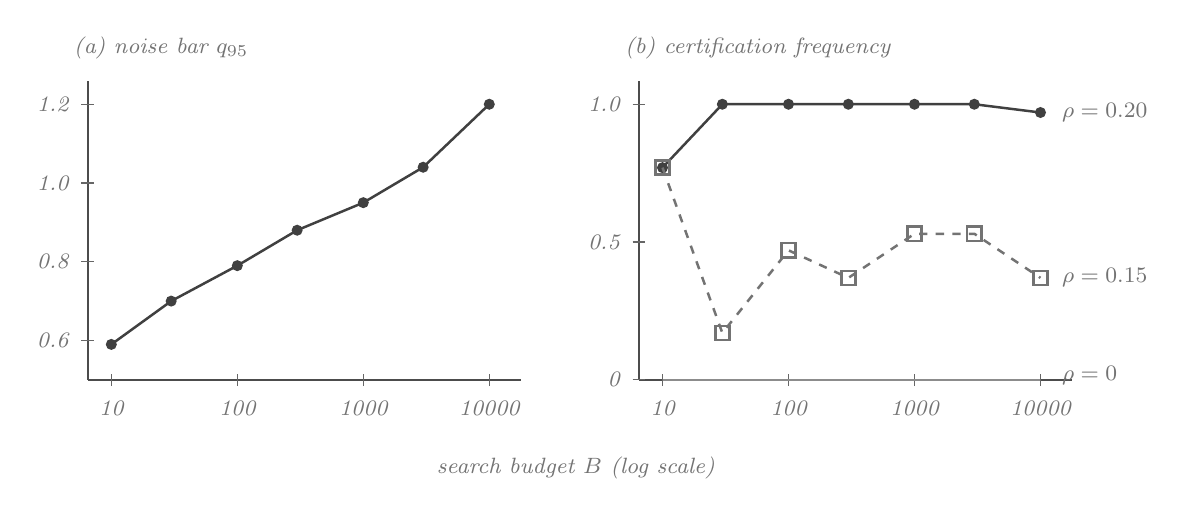
\begin{tikzpicture}[font=\small]
  \node[annot, anchor=south west] at (0.0,3.95) {(a) noise bar $q_{95}$};
  \draw[black!70, line width=0.8pt] (0.3,0) -- (0.3,3.8);
  \draw[black!70, line width=0.8pt] (0.3,0) -- (5.8,0);
  \foreach \y/\l in {0.5/0.6, 1.5/0.8, 2.5/1.0, 3.5/1.2} {
    \draw[black!60] (0.22,\y) -- (0.38,\y);
    \node[annot, anchor=east] at (0.18,\y) {\l};
  }
  \foreach \x/\l in {0.6/10, 2.2/100, 3.8/1000, 5.4/10000} {
    \draw[black!60] (\x,-0.08) -- (\x,0.08);
    \node[annot, anchor=north] at (\x,-0.15) {\l};
  }
  \draw[black!75, line width=0.9pt] (0.6,0.45) -- (1.36,1.0) -- (2.2,1.45) -- (2.96,1.9)
    -- (3.8,2.25) -- (4.56,2.7) -- (5.4,3.5);
  \foreach \p in {(0.6,0.45),(1.36,1.0),(2.2,1.45),(2.96,1.9),(3.8,2.25),(4.56,2.7),(5.4,3.5)}
    \fill[black!75] \p circle (2pt);
  \node[annot, anchor=south west] at (7.0,3.95) {(b) certification frequency};
  \draw[black!70, line width=0.8pt] (7.3,0) -- (7.3,3.8);
  \draw[black!70, line width=0.8pt] (7.3,0) -- (12.8,0);
  \foreach \y/\l in {0/0, 1.75/0.5, 3.5/1.0} {
    \draw[black!60] (7.22,\y) -- (7.38,\y);
    \node[annot, anchor=east] at (7.18,\y) {\l};
  }
  \foreach \x/\l in {7.6/10, 9.2/100, 10.8/1000, 12.4/10000} {
    \draw[black!60] (\x,-0.08) -- (\x,0.08);
    \node[annot, anchor=north] at (\x,-0.15) {\l};
  }
  \draw[black!75, line width=0.9pt] (7.6,2.695) -- (8.36,3.5) -- (9.2,3.5) -- (9.96,3.5)
    -- (10.8,3.5) -- (11.56,3.5) -- (12.4,3.395);
  \foreach \p in {(7.6,2.695),(8.36,3.5),(9.2,3.5),(9.96,3.5),(10.8,3.5),(11.56,3.5),(12.4,3.395)}
    \fill[black!75] \p circle (2pt);
  \draw[black!55, dashed, line width=0.9pt] (7.6,2.695) -- (8.36,0.595) -- (9.2,1.645) -- (9.96,1.295)
    -- (10.8,1.855) -- (11.56,1.855) -- (12.4,1.295);
  \foreach \x/\y in {7.6/2.695,8.36/0.595,9.2/1.645,9.96/1.295,10.8/1.855,11.56/1.855,12.4/1.295}
    \draw[black!55, line width=0.9pt] (\x-0.09,\y-0.09) rectangle (\x+0.09,\y+0.09);
  \draw[black!45, line width=0.9pt] (7.6,0) -- (12.4,0);
  \node[annot, anchor=west] at (12.55,3.4) {$\rho=0.20$};
  \node[annot, anchor=west] at (12.55,1.3) {$\rho=0.15$};
  \node[annot, anchor=west] at (12.55,0.05) {$\rho=0$};
  \node[annot, anchor=north] at (6.5,-0.85) {search budget $B$ (log scale)};
\end{tikzpicture}
\caption{The budget sweep of Table~\ref{tab:capacity}. (a) The bar measured on noise rises steadily as
the budget grows from 10 to 10{,}000 candidates. (b) Certification frequency against the budget-matched
bar: zero at $\rho=0$ at every budget, at or near one at $\rho=0.20$, and fluctuating with no trend at the
threshold strength $\rho=0.15$.}
\label{fig:capacity}
\end{figure}

Figure~\ref{fig:capacity} plots the sweep. The noise bar rises steadily with budget, from 0.59 at ten
candidates to 1.20 at ten thousand, with no plateau. The certification frequency on noise ($\rho=0$)
stays at 0 of 30 at every budget on this realization, because the bar is recomputed from the same search on scrambled returns
and so rises with it. For a threshold signal ($\rho=0.15$) the champion scores and the bar rise together,
and the certification frequency fluctuates between 0.17 and 0.77 with no trend. A clear signal
($\rho=0.20$) is certified in 30 of 30 runs at every budget from 30 to 3{,}000, in 29 of 30 at 10{,}000,
and in 23 of 30 at the smallest budget of 10.

The bar therefore rises with budget, and in the tested range this rise did not reduce detection: a
larger budget raised the champion's score as much as it raised the bar. Four qualifications apply. The
class is the finite random-tree family, not the unbounded code-writing class of Eq.~\eqref{eq:vc}. The
false-positive result holds in part by construction, since a bar recomputed for the same search fixes
the false-positive rate at any budget. Budgets beyond ten thousand candidates are untested. And the
sign-flip null tests directional signal, which is valid for this long-only selection task, where all
profit and loss is directional, but need not hold for a class with a non-directional route to fitting
noise.

\subsection{LLM and mechanical search (E7)}
\label{sec:e7}

The LLM arm uses a Claude Opus subagent to propose each structure (Section~\ref{sec:design}). We run 3
seeds at each of three signal levels and report the champion scores next to the median champion of the
mechanical nonlinear search at the same $\rho$ (Table~\ref{tab:llm}). No bar was computed for the LLM
search, so these scores are not certified; the nonlinear bar of 0.844 is shown only as a reference.

\begin{table}[htbp]
\centering
\caption{Champion scores of the LLM search (three runs per $\rho$) and the median champion of the
mechanical nonlinear search (30 runs, E1). The LLM scores are not certified, because no bar was computed
for the LLM search.}
\label{tab:llm}
\small
\begin{tabular}{c c c}
\toprule
$\rho$ & LLM champion scores & mechanical median champion \\
\midrule
0.00 & 0.52,\ 0.22,\ $-0.05$ & 0.44 \\
0.15 & 0.82,\ 0.91,\ 0.36 & 0.83 \\
0.20 & 1.22,\ 1.02,\ 1.40 & 1.10 \\
\bottomrule
\end{tabular}
\end{table}

\begin{figure}[htbp]
\centering
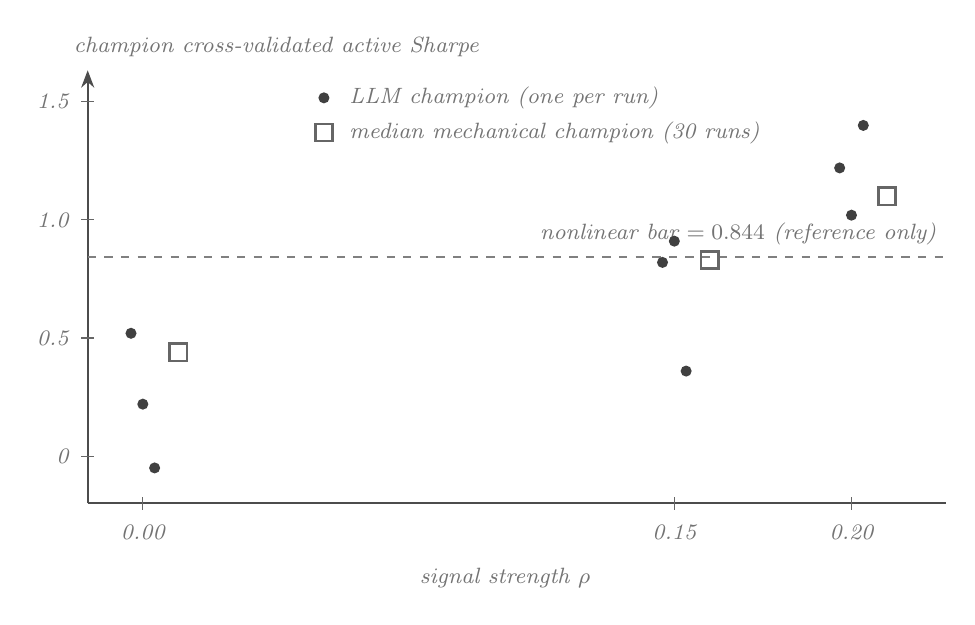
\begin{tikzpicture}[font=\small]
  \draw[black!70, line width=0.8pt, -{Stealth[length=2.2mm]}] (0.3,-0.6) -- (0.3,4.9);
  \node[annot, anchor=south west] at (0.0,4.95) {champion cross-validated active Sharpe};
  \foreach \y/\l in {0/0, 1.5/0.5, 3.0/1.0, 4.5/1.5} {
    \draw[black!60] (0.22,\y) -- (0.38,\y);
    \node[annot, anchor=east] at (0.18,\y) {\l};
  }
  \draw[black!70, line width=0.8pt] (0.3,-0.6) -- (11.2,-0.6);
  \foreach \x/\l in {1/0.00, 7.75/0.15, 10/0.20} {
    \draw[black!60] (\x,-0.68) -- (\x,-0.52);
    \node[annot, anchor=north] at (\x,-0.75) {\l};
  }
  \node[annot, anchor=north] at (5.6,-1.3) {signal strength $\rho$};
  \draw[dashed, black!50, line width=0.8pt] (0.3,2.532) -- (11.2,2.532);
  \node[annot, anchor=south east] at (11.2,2.56) {nonlinear bar $=0.844$ (reference only)};
  \fill[black!75] (0.85,1.56) circle (2pt);
  \fill[black!75] (1.0,0.66) circle (2pt);
  \fill[black!75] (1.15,-0.15) circle (2pt);
  \fill[black!75] (7.6,2.46) circle (2pt);
  \fill[black!75] (7.75,2.73) circle (2pt);
  \fill[black!75] (7.9,1.08) circle (2pt);
  \fill[black!75] (9.85,3.66) circle (2pt);
  \fill[black!75] (10.0,3.06) circle (2pt);
  \fill[black!75] (10.15,4.20) circle (2pt);
  \draw[black!60, line width=0.9pt] (1.34,1.21) rectangle (1.56,1.43);
  \draw[black!60, line width=0.9pt] (8.09,2.38) rectangle (8.31,2.60);
  \draw[black!60, line width=0.9pt] (10.34,3.19) rectangle (10.56,3.41);
  \fill[black!75] (3.3,4.55) circle (2pt);
  \node[annot, anchor=west] at (3.5,4.55) {LLM champion (one per run)};
  \draw[black!60, line width=0.9pt] (3.19,4.00) rectangle (3.41,4.22);
  \node[annot, anchor=west] at (3.5,4.11) {median mechanical champion (30 runs)};
\end{tikzpicture}
\caption{The E7 comparison of Table~\ref{tab:llm}. Each filled circle is the champion score of one LLM
run; each open square is the median champion of the 30 mechanical runs at the same $\rho$ (E1). The
dashed line is the nonlinear bar, shown for scale; it is not the matched bar for the LLM search, so the
LLM points are not certified by it.}
\label{fig:llm}
\end{figure}

The LLM champions scored in the same range as the mechanical champions at each signal strength, and at
$\rho>0$ every LLM champion used \code{feat\_c}, the true predictor. With three runs per point this shows
that the model works as a proposer in the loop; it does not show equivalence with mechanical search, and
it cannot show an advantage, because the four features have no meaningful names for the model's prior to
use. Two further limits apply. The runs at seeds 1 and 2 used a different noise realization from E1, so
the comparison with the mechanical medians is approximate. And the champion of the $\rho=0$, seed-0 run
(score 0.52) read the raw price series, which the prompt forbids, through a lookback of 285 trading days,
longer than the embargo; the harness accepted it because it checks compilation, not inputs.

\subsection{Implementation}
\label{sec:impl}

Each LLM search runs up to 12 proposal rounds, seeded with simple feature-combination structures. A
candidate's parameters are fit by differential evolution (SciPy's implementation with population
multiplier 8, so the population is 8 times the number of parameters, a nominal budget of 60 evaluations,
mutation weight sampled in $[0.5,1.0]$, and recombination 0.7). The prompt is a fixed task contract plus
the scored history of up to twelve prior structures, strongest first, and the model returns one new
structure. Each request is written to a file and serviced by a Claude Opus subagent of the Claude Code
session, which writes its answer back. The temperature argument is not passed on this path, and the
subagent's sampling settings are unknown and were not logged. The subagents were launched by the same
interactive session that built the test-bed, with instructions to read each request file and write a
response; the launch instructions were not logged, so we cannot exclude that they, or the subagent's own
file access, conveyed which feature carries the signal. The prompts give
the model the task contract, the four feature names, and prior structures with their cross-validated
scores, and no prices, returns, or feature values. The mechanical searchers use no model and share the
rest of the stack.

\subsection{Findings}
\label{sec:findings}

The experiments answer one question: does the loop work as a measurement tool on this test-bed? The
measured facts are these.

\begin{itemize}[leftmargin=1.4em]
\item \textbf{Detection.} The nonlinear search certifies reliably from $\rho=0.20$, where the planted
feature alone is worth an active Sharpe of about 0.83 (0.95 for the realization searched); it is
unreliable at $\rho=0.15$ (13 of 30) and finds nothing weaker. The linear search becomes reliable at
$\rho=0.30$.
\item \textbf{Noise rejection.} With a new noise realization for each of 30 runs, neither search
certified pure noise (false-positive rate below 9.5\% at 95\% confidence), and on the single realization
of E4 the count stayed at 0 of 30
at every budget from 10 to 10{,}000 candidates.
\item \textbf{The bar belongs to the search.} On identical data the nonlinear bar is 0.844 and the linear
bar 0.408.
\item \textbf{Scores are inflated.} At $\rho=0.20$ the median champion scored 1.10 against an oracle of
0.95 for the same data.
\item \textbf{A mismatched bar fails.} Judged against the linear bar, 13 of 30 pure-noise champions of
the nonlinear search pass on independent realizations (20 of 30 on the single realization of E5);
against their own bar, none do.
\item \textbf{Budget.} The bar rose from 0.59 to 1.20 as the budget grew from 10 to 10{,}000, without
false positives and without loss of detection at $\rho=0.20$.
\item \textbf{Language model.} Its champions scored in the same range as mechanical search on opaque
features; they were not certified.
\end{itemize}

These statements hold for this synthetic test-bed, with in-sample certification against the null-max
bar, the directional sign-flip null, and the stated families and budgets. They establish that the loop
detects signal present in its supplied features. Whether a real feature set contains such signal is a
separate question, which the loop can test but cannot answer on its own.

\section{The limits of automated alpha search}
\label{sec:ceiling}

LATSS searches and certifies strategies over a feature vocabulary that a human supplies, and whether
it produces alpha depends on whether those features predict. The question is whether the vocabulary
itself can be automated, whether an LLM system can invent new alpha. By inventing new alpha we do not
mean producing a factor formula nobody has published, which a search system does easily. We mean
originating a new hypothesis about where returns come from: a variable, mechanism, or relationship
outside the space the system was given. This is a stronger property than producing outputs that people
judge novel, which we take up in Section~\ref{sec:invention}. Alpha that is new to the market but built
from kinds of variables the model already knows is a different and weaker target, taken up in
Section~\ref{sec:looptoinvention}; this section concerns invention in the strong sense.

\subsection{Search and abduction}
\label{sec:formal}

The distinction that matters in this section is between two acts. \emph{Search} is picking the best
candidate out of a given collection: there is a set of possible strategies, a score for each, and the
searcher returns the highest-scoring one it finds. This is what LATSS does, what FunSearch does, and
what LLM factor-mining systems do. \emph{Abduction} is producing a candidate the given collection does
not contain: extending the collection when nothing inside it explains the phenomenon. Search
presupposes that the collection worth searching has already been supplied; abduction is what supplies
it.

Now apply the distinction to a language model used as a proposer. The model was trained on a body of
text and code, and everything it proposes is some recombination or re-expression of what that training
material contains. Call the set of everything reachable this way the model's \emph{reachable set},
written $\mathcal{C}(D)$, where $D$ stands for the training material. The term is a conceptual
abstraction, a way of talking about what recombination can reach, not a set anyone can measure.

In the LATSS loop the model is used to draw candidates, and the draw can be written as
\begin{equation}
s \;\sim\; P_{\theta}\bigl(s \mid x, \mathcal{V}\bigr).
\label{eq:proposal}
\end{equation}
The symbols mean the following.
\begin{itemize}[leftmargin=1.4em]
\item $s$ is one candidate strategy, the Python scoring function the model writes.
\item $\sim$ means ``is drawn at random from''.
\item $P_{\theta}$ is the language model itself, viewed as a probability distribution over the text it can
emit; $\theta$ stands for its trained weights, which are fixed and do not change during the search.
\item $x$ is the prompt: the task description and the code and scores of earlier candidates.
\item $\mathcal{V}$ is the feature vocabulary, the set of input signals the strategy is allowed to read.
\item The vertical bar ``$\mid$'' means ``given'': the distribution over strategies depends on the prompt
and the vocabulary.
\end{itemize}
Two facts follow from the equation. First, every candidate is built from the features in $\mathcal{V}$,
so a relationship that cannot be expressed with those features is never proposed, whatever the model
knows. Second, a strategy to which $P_{\theta}$ gives zero or negligible probability under every prompt the
loop can build is, in practice, never drawn; the reachable set $\mathcal{C}(D)$ is the informal name for
the strategies that receive appreciable probability. The prompt $x$ shifts probability among those
strategies, which is how the loop's feedback steers the search, but it does not change $\theta$.

Two consequences follow. First, if the collection being searched lies inside the reachable set, then
every proposal, and therefore every champion, lies inside it too. Novelty of that kind is routine: the
model emits formulas nobody has written down, but each one is a recombination of what it was trained
on, which is interpolation, not invention. Second, enlarging the search does not escape the set. Asking
the model for new variables, new datasets, or new ideas enlarges the collection being searched, but the
suggestions still come from the reachable set, each a recombination of hypotheses already present in
the training material. The abductive target is, by definition, a hypothesis the reachable set does not
contain, and searching inside the set does not produce one. A hypothesis inside the set can still be
new to the market, which is the case Section~\ref{sec:looptoinvention} develops. The limit on
invention is the content of Zahavy's
\emph{LLMs Can't Jump}~\cite{zahavy}. The claim concerns the content of hypotheses, not geometry:
Balestriero, Pesenti, and LeCun show that in high dimension new inputs almost always fall outside the
convex hull of the training data, so ``extrapolation'' in that geometric sense is routine~\cite{lecun};
producing a point outside a set of examples is not the same as introducing a concept the examples do
not contain.

\subsection{FunSearch}

The strongest apparent counterexample is FunSearch~\cite{funsearch}, where an LLM coupled to an
evaluator found previously unknown constructions. The human supplies the problem, the evaluation
function, and the representation, and the system then generates on the order of a million candidates
and keeps the best. FunSearch shows that an LLM can participate in discovery. It does not show the
LLM deciding what should be discovered. It did not conclude that a different representation was needed
and invent it; it searched very well inside a space a human defined.

\subsection{Creating a search space}

Zahavy's example is Einstein's route to general relativity: the equivalence principle was a new premise
that changed what counted as a valid explanation, and so created a space of theories to search rather
than a better point in an existing one~\cite{zahavy}. Figure~\ref{fig:jump} draws the distinction.

\begin{figure}[htbp]
\centering
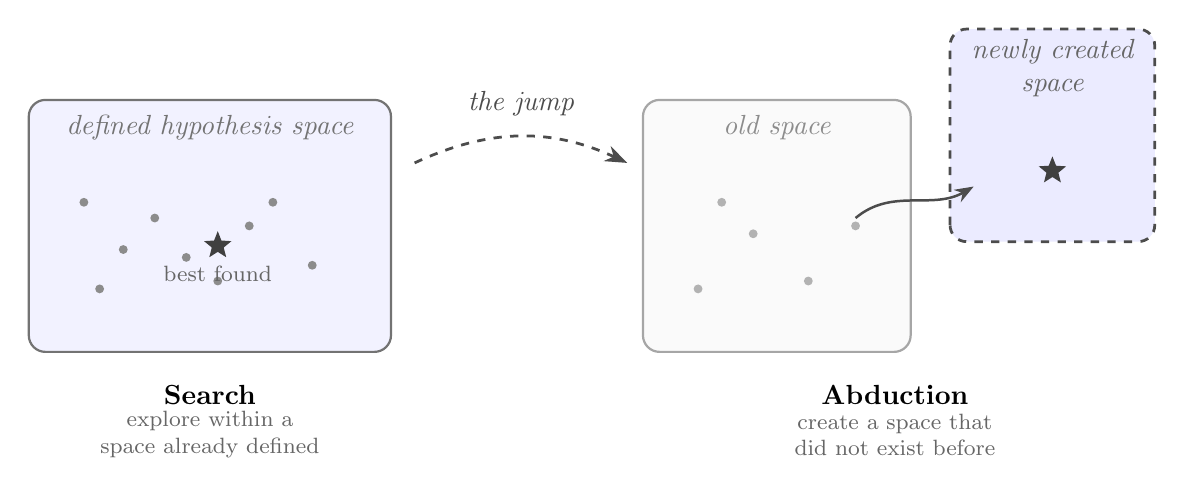
\begin{tikzpicture}[font=\small]
  \begin{scope}[shift={(0,0)}]
    \draw[rounded corners=6pt, draw=black!55, fill=blue!5, line width=0.8pt] (0,0) rectangle (4.6,3.2);
    \node[font=\itshape, text=black!55] at (2.3,2.85) {defined hypothesis space};
    \foreach \p in {(0.9,0.8),(1.6,1.7),(2.4,0.9),(3.1,1.9),(2.0,1.2),(3.6,1.1),(1.2,1.3),(2.8,1.6),(0.7,1.9)}
      \fill[black!45] \p circle (1.6pt);
    \node[star, star points=5, star point ratio=2.3, fill=black!75, inner sep=1.6pt] (best) at (2.4,1.35) {};
    \node[font=\footnotesize, text=black!60, below=0.5mm of best] {best found};
    \node[font=\bfseries] at (2.3,-0.55) {Search};
    \node[font=\footnotesize, text=black!60, align=center] at (2.3,-1.05) {explore within a\\ space already defined};
  \end{scope}
  \draw[-{Stealth[length=2.8mm]}, line width=1pt, draw=black!70, dashed] (4.9,2.4) to[out=25,in=155] (7.6,2.4);
  \node[font=\itshape, text=black!70] at (6.25,3.15) {the jump};
  \begin{scope}[shift={(7.8,0)}]
    \draw[rounded corners=6pt, draw=black!35, fill=black!2, line width=0.8pt] (0,0) rectangle (3.4,3.2);
    \node[font=\itshape, text=black!45] at (1.7,2.85) {old space};
    \foreach \p in {(0.7,0.8),(1.4,1.5),(2.1,0.9),(2.7,1.6),(1.0,1.9)} \fill[black!30] \p circle (1.6pt);
    \draw[rounded corners=6pt, draw=black!70, fill=blue!8, line width=1pt, dashed] (3.9,1.4) rectangle (6.5,4.1);
    \node[font=\itshape, text=black!60, align=center] at (5.2,3.6) {newly created\\ space};
    \node[star, star points=5, star point ratio=2.3, fill=black!75, inner sep=1.6pt] at (5.2,2.3) {};
    \draw[-{Stealth[length=2.4mm]}, line width=0.9pt, draw=black!70] (2.7,1.7) to[out=40,in=210] (4.2,2.1);
    \node[font=\bfseries] at (3.2,-0.55) {Abduction};
    \node[font=\footnotesize, text=black!60, align=center] at (3.2,-1.05) {create a space that\\ did not exist before};
  \end{scope}
\end{tikzpicture}
\caption{Search explores within a hypothesis space already defined. Abduction creates a space that
did not exist, the step an LLM has not been shown to take.}
\label{fig:jump}
\end{figure}

\subsection{Evidence on machine invention}
\label{sec:invention}

Two questions should be kept apart. The first is whether LLMs can produce outputs that people judge
novel. They can. In a controlled study with more than one hundred NLP researchers, Si, Yang, and
Hashimoto found that LLM-generated research ideas were rated more novel than those of human experts,
though less feasible~\cite{si2024}. A system named The AI Scientist, published by Sakana AI, automates
much of the research loop, generating ideas, writing and running code, and producing manuscripts, and
reports experimentally evaluated contributions~\cite{aiscientist}. This is novelty of output.

The second question is whether an LLM has independently originated a new explanatory hypothesis whose
conceptual content was not already present in its training distribution, its prompt, its search
vocabulary, or a human-designed experimental frame. Here the evidence is thin. The reported novelty is
measured against a literature corpus or human judgment, and the autonomous systems run inside
substantial human scaffolding. An independent evaluation of that system found that it often
labeled established techniques as novel and that many of its experiments and manuscripts were
flawed~\cite{aiscientisteval}. In a controlled molecular-genetics setting, Ding and Li report that a
generative model made incremental discoveries but not fundamental ones from scratch and did not
produce genuinely original hypotheses~\cite{dingli}. Zahavy frames the same gap as a missing abductive
step and takes Einstein's route to general relativity as the case~\cite{zahavy}.

The distinction is between novelty of output and novelty of hypothesis. The first is increasingly
demonstrated. The second remains open, and to our knowledge no published result has established it
with provenance showing the hypothesis was not inherited from the training data or the search frame.
LATSS does not settle the question. Section~\ref{sec:e12a} tests one part of it: when the predictive
feature is withheld from the vocabulary, more search does not recover it, because search cannot
recover information absent from the space it is given. An LLM may find a new solution inside a
financial hypothesis space without finding a new reason the market behaves as it does; the first is a
search problem, the second is the invention problem.

\subsection{The supplied vocabulary in alpha search}

Everything is decided before the search: which data is relevant, the prediction target, the horizon,
the available transformations, the evaluator, and the tests of success. A factor miner handed RSI,
volume, volatility, and momentum can find an expression nobody has written, and it remains a
construction from the given vocabulary. When the source of an anomaly is a variable that is not in
the vocabulary, not among the available transformations, and not in the database, searching the given space
harder does not surface it, because the missing ingredient is outside the space. More compute, more
agents, deeper tree search, and a larger context window do not change this.

\subsection{Proposing new variables}

One response is to move the search up a level and ask the model for new variables and mechanisms,
which it supplies fluently: filing sentiment, supplier networks, options positioning. Such proposals
typically recombine hypotheses already discussed in the literature. A variable proposed this way can be
new to a given strategy, and possibly new to the market, without being a concept new to the world; the
first two are the targets of Section~\ref{sec:looptoinvention}, and only the last is invention in the
strong sense.

\subsection{Two ceilings}
\label{sec:two-ceilings}

We argue that alpha resists automated discovery for two independent reasons. The first is a cognitive
ceiling: a model sampling from a fixed distribution has not been shown to produce a hypothesis outside
$\mathcal{C}(D)$ (Section~\ref{sec:formal}). LeCun's critique that LLMs have no world model~\cite{lecunmtr} is a separate limitation
that scaffolding can address: LATSS supplies an external check, the backtest against data, in place of
an internal model of the market. Grounding tells the model whether a hypothesis
it already holds survives the data; it does not generate a hypothesis outside $\mathcal{C}(D)$. The
market-structure ceiling is that alpha is adversarial and perishable and its evaluator is causally
ambiguous: a successful backtest does not say why a factor predicted, whether mechanism, correlation,
hidden risk, regime, leakage, cost, or crowding. A new mechanism is necessary but not sufficient for
durable alpha, and the bar addresses overfitting within the search, not the missing hypothesis.

\subsection{Levels of novelty}
\label{sec:novelty}

Novelty covers four distinct achievements (Table~\ref{tab:novelty}), which lets a claim be held to a
matching standard of evidence. The first two can be reached by search within a supplied space. The
hypothesis level requires evidence that the explanation was not already present in the model's
training or inputs. The economic level is a separate axis: an edge can be new to the market and durable
whether or not the idea behind it is new to the world.

\begin{table}[htbp]
\centering
\caption{Levels of novelty in automated alpha discovery. Only the hypothesis level requires a
hypothesis outside the model's reachable set $\mathcal{C}(D)$; economic novelty concerns the market, not
the idea.}
\label{tab:novelty}
\small
\begin{tabular}{@{}p{2.3cm} p{3.9cm} p{4.1cm} p{2.4cm}@{}}
\toprule
level & definition & evidence that would demonstrate it & state \\
\midrule
Syntactic & a formula no one has written & any run emitting a novel expression & routine \\[2pt]
Solution & a new construction for a defined problem & FunSearch cap-set and bounds~\cite{funsearch} & demonstrated \\[2pt]
Hypothesis & a new explanation for an unexplained phenomenon & a system originating a driver no source in $D$ contains, with a positive control & not demonstrated \\[2pt]
Economic & a new, durable, uncrowded source of returns & an edge proposed by the system that survives forward testing after costs and crowding & none reported \\
\bottomrule
\end{tabular}
\end{table}

The claim that no current system has been shown to reach the hypothesis level is falsifiable. It is
refuted by a system that originates an explanation of returns that no source in its training data
contains, with a positive control showing the step was achievable; the benchmark of
Section~\ref{sec:jumpbench} specifies such a test. We found no such demonstration. The economic level is
open for a different reason: it requires forward testing that no LLM alpha system we found has
reported.

\subsection{Current systems}
\label{sec:audit}

Table~\ref{tab:audit} places representative systems by search space and novelty level. The level is a
qualitative classification we argue from each system's design, not a bibliographic fact. Each
recombines a human-defined primitive vocabulary, and we found no published demonstration of one
originating an economic primitive no one specified. AlphaAgent adds a penalty on syntax-tree similarity
to known factors~\cite{alphaagent}, which shows that its authors expected unregularized generation to
reproduce known factors.

\begin{table}[htbp]
\centering
\caption{Representative LLM alpha systems by search space and novelty level (as in
Table~\ref{tab:novelty}); the level is a qualitative classification argued here. ``1--2'' means
syntactic novelty is evident and solution-level novelty is not established by the published results.
LATSS recovered a planted signal, which is level 1.}
\label{tab:audit}
\small
\begin{tabular}{@{}p{3.3cm} p{5.3cm} p{2.1cm} p{1.4cm}@{}}
\toprule
system & primitive vocabulary / search space & machinery & level \\
\midrule
LATSS (this work) & given indicators to scoring rule & differential evolution, null-max bar & 1 \\
AlphaAgent~\cite{alphaagent} & factor formulas over raw price/volume & multi-agent, syntax-tree penalty & 1--2 \\
Automate Strategy Finding~\cite{automate} & factor/strategy formulas over raw inputs & multi-agent & 1--2 \\
CogAlpha~\cite{cogalpha} & factor code over raw inputs & LLM, evolutionary search & 1--2 \\
QuantaAlpha~\cite{quantaalpha} & factor formulas over raw inputs & multi-agent & 1--2 \\
AlphaLogics~\cite{alphalogics} & logic and formula factors & search, verify & 1--2 \\
EFS~\cite{efs} & evolutionary factor formulas & evolutionary search & 1--2 \\
FunSearch~\cite{funsearch} (math) & programs for a defined problem & LLM, exact evaluator & 2 \\
\bottomrule
\end{tabular}
\end{table}

\subsection{Withholding the predictive feature (E12a)}
\label{sec:e12a}

This experiment is a sanity check whose outcome is fixed by construction; we include it because it makes
the vocabulary boundary concrete. We inject the signal into \code{feat\_c} as in
Section~\ref{sec:e1}, then overwrite the searcher's \code{feat\_c} with independent noise, so the
predictive feature is absent from the vocabulary. Across $\rho$ from 0 to 0.70, 30 seeds each, the
certification rate is zero at every signal strength, with the champion median between 0.43 and 0.53 against a bar
of 0.844. Section~\ref{sec:e1}, with \code{feat\_c} present, recovers reliably from $\rho=0.20$.
Recovery is governed by whether the predictive feature is in the vocabulary, not by signal strength
or search effort. We state the limit of this result directly: a mechanical searcher fails the same
way, and so would a human analyst given only the same four columns, so it demonstrates the vocabulary
boundary and not an LLM-specific inability. No proposer can construct a variable that is absent from the
data it is given. The claim of this paper is therefore not that a language model fails where other
methods succeed. It is that a proposer without a mechanism for extending its inputs, such as a tool that
requests a new measurement or data source, is confined to combinations of the vocabulary it was given, and
that whether a language-model agent equipped with such a tool requests the right measurement is an open,
measurable question (Section~\ref{sec:jumpbench}). A test that
isolates the LLM-specific step would need a semantically nameable driver together with a human or
oracle positive control, which the opaque synthetic driver here cannot provide, and we leave it to
future work.

\subsection{Search and invention in current systems}

LATSS is the alpha analogue of a coding agent: it generates, validates, and recombines strategies from a
human-supplied vocabulary under human supervision, scored against the backtest much as a coding agent is
scored against its tests. Like the systems of Table~\ref{tab:audit}, it searches and certifies over
supplied primitives. A system that, given raw data and no predefined vocabulary, repeatedly finds durable,
economically intelligible returns that no source told it to look for would be doing something different.
We found no such demonstration.

\section{Toward abduction of alpha}
\label{sec:abduction}

The ultimate goal is a system that discovers new alpha, which is a special case of scientific
discovery: a durable economic edge rests on a new explanation of why a market behaves as it does. To
aim at that goal we ask how human discovery works, locate where a language model can and cannot
contribute, and give a concrete benchmark that would make progress measurable.

\subsection{The structure of scientific discovery}
\label{sec:philsci}

Accounts of discovery in the philosophy of science converge on a two-part structure. Peirce separated
three modes of inference: deduction draws out consequences, induction generalizes from instances, and
\emph{abduction} generates an explanatory hypothesis to account for a surprising observation; only
abduction introduces a new idea, and Peirce described the abductive suggestion as coming to us
``like a flash,'' an act of insight~\cite{peirce}. Hanson made abduction a logic of discovery and stressed that inquiry starts
from an anomaly, an observation the current frame does not predict~\cite{hanson}. Popper denied that
there is any logic for producing the hypothesis at all: science proceeds by \emph{conjectures and
refutations}, bold guesses exposed to attempted falsification, with the generation of the conjecture
left to the scientist and only its testing governed by method~\cite{popper}. Kuhn distinguished normal
science, puzzle-solving inside an accepted paradigm, from revolutionary science, where the paradigm
itself is replaced~\cite{kuhn}; Lakatos recast this as research programmes with a protected hard
core~\cite{lakatos}; and Schurz catalogued the kinds of abductive guess, from factual to
theoretical-model abduction~\cite{schurz}. Computational work matches the division: the BACON system of
Langley and Simon rediscovered quantitative laws by heuristic search over a supplied representation,
which is discovery at the level of a new construction inside a given vocabulary rather than a new
vocabulary~\cite{bacon}.

Two points are common to these accounts. Discovery is conjecture plus test, iterated at scale: a guess is proposed, often
triggered by an anomaly, and is then kept or discarded by confronting it with evidence, and the rare
surviving guess is the discovery. And the creative content is the conjecture, which Peirce and Popper treat as
outside method, while the testing is the part method can systematize; the computational tradition of
BACON holds that some conjectures can be produced by heuristic search.

\subsection{The language model in the discovery cycle}
\label{sec:inference-loop}

Where the language model fits in this structure depends on what a transformer is. At
inference a trained transformer is a fixed function from a context to a distribution over
continuations. Its weights are frozen, and it carries no state between calls; the only memory it has is
what is placed in its context window. Persistence, accumulation of results, and iteration are therefore
not properties of the model but of the agent built around it.

\paragraph{The transformer at inference.} A decoder-only transformer maps a token sequence through an
embedding, a stack of self-attention and feed-forward blocks with residual connections, and a final
projection and softmax, producing a probability distribution over the next token. Generation is
autoregressive: a token is sampled, appended to the context, and the pass repeats. The parameters do
not change during this process, and the key-value cache that makes generation efficient is internal to a
single sequence and is discarded between calls. In-context learning conditions the same fixed function
on a longer input without updating any weight; how much new capability such conditioning can produce is
an open research question, but it leaves the weights unchanged. The weights are fixed, so the conditional distribution the model samples
from is set by training and by the context it is given, and its reach is, as a conceptual abstraction,
the recombination closure $\mathcal{C}(D)$ of Section~\ref{sec:formal}. Sampling can produce token
sequences no one has written, which is the syntactic and solution novelty of Table~\ref{tab:novelty},
yet sampling from a fixed model provides no explicit mechanism for creating a hypothesis whose relevant
conceptual content is absent from the model's learned representation. A softmax model gives every
sequence some nonzero probability, so the relevant limit is practical: raising the temperature makes
low-probability continuations more likely but does not make likely those the model assigns negligible
probability under every context the loop can build. Chain-of-thought
and tool use lengthen and externalize the computation, and each added step is another conditioned
forward pass, so they deepen deduction and search, and we argue that they do not move the model outside
$\mathcal{C}(D)$. This is the
basis of the argument below: the single operation available to the model, sampling a continuation from a
fixed conditional distribution, is not an operation designed to create a hypothesis outside that
distribution.

Mapping this onto the discovery cycle, the model supplies the conjecture step, sampling a candidate
from its reachable set $\mathcal{C}(D)$ (Section~\ref{sec:formal}). The agent supplies the rest: the
anomaly that prompts a conjecture, the memory of what has been tried, and the test that refutes or
retains it. In LATSS the evaluator and the null-max bar are that test, a mechanized refutation step.
The loop is thus conjecture and refutation run at scale, with the model generating guesses and the bar
refuting them.

The framing explains both the value and the limit. The test is validated on the synthetic test-bed of
Sections~\ref{sec:framework} to~\ref{sec:results}, so an agent can generate and refute conjectures far
faster than a human. But a sampler over $\mathcal{C}(D)$ proposes guesses from inside its own
distribution, so scaling the loop produces more conjectures of the same kind and more tests, which is
Kuhn's normal science. The abductive jump is a conjecture to which the distribution gives negligible
probability. Progress toward invention is therefore progress on the conjecture step, not the test.

\paragraph{Invention is not inference.} An inference engine maps an input to an output within a learned
distribution; a jump is the creation of a hypothesis outside that distribution, which is a different
kind of act. We argue that this difference, not a lack of scale, is why current models have not been
shown to invent; the argument is falsifiable by the benchmark of Section~\ref{sec:jumpbench}. If it is
right, whatever performs the jump must sit outside the inference step. On this reading the language model's role is to \emph{assist} invention, not to perform it: it is a fast
generator of conjectures inside its reach and a competent executor of the search and coding that
discovery also requires, while originating a genuinely new hypothesis, and the agent architecture that
might one day carry it, lies outside the model. LATSS is built on this division. The model proposes and
the surrounding loop tests; we neither ask nor expect the model itself to originate a concept outside its training, and a
system that one day does so will have placed the generative step in the agent that wraps the model, not
in the model.

\subsection{Invention as an agent-level capability}
\label{sec:agent}

If invention happens at all, it must be a property of the agent, with the model as one component.
Operationally that agent is a conjecture-and-refutation loop of two stages, a proposal stage that
generates a candidate hypothesis and a validation stage that keeps or discards it, iterated. LATSS is
already this loop, and its validation stage, certification against the null-max bar, is the part this
paper validates. The underdeveloped half is the proposal stage.

The true hypothesis may lie inside the supplied hypothesis space or outside it. Inside, finding it is
ordinary search, and the model helps. Outside the supplied vocabulary, no search over the supplied space
reaches it, and the agent's task then also includes enlarging the space. Even inside the space,
enumerating every hypothesis is infeasible, so the agent needs a proposal heuristic, a prior that says
which conjectures are worth testing first; Peirce called abduction the economy of research for this
reason~\cite{peirce}. The model's training distribution supplies such a prior, and the next subsection
develops what it can and cannot do. The two missing capabilities for invention are therefore a way to
enlarge the hypothesis space and a prior that favors promising but uncrowded hypotheses; the benchmark of
Section~\ref{sec:jumpbench} measures the first.

\subsection{The language model as a prior over hypotheses}
\label{sec:prior}

A trained language model assigns probabilities to text. Given a description of the task and the names
of the available features, it can do two things a mechanical searcher cannot: generate a large number of
candidate hypotheses about what drives returns, and assign each one a plausibility. The plausibility can
be obtained by asking the model for a probability, by asking it to rank candidates against one another,
or by reading off the likelihood the model assigns to the text of each hypothesis. Whichever method is
used, the result is a prior over hypotheses in the sense of Tarantola's procedure
(Section~\ref{sec:inverse}): a distribution, formed before the data is examined, that says which models
are worth testing first. Peirce placed the value of abduction in exactly this choice of which guess to
try~\cite{peirce}.

\paragraph{The argument for ranking.} Testing a hypothesis is not free in statistical terms. The
budget experiment (Section~\ref{sec:e4}) measured that the bar rises with the number of candidates a
search evaluates, because more attempts on noise produce a higher best-on-noise score. The conjecture is
that a prior which lets the loop test only the top-ranked few hypotheses pays a lower bar than blind
enumeration of many, so that a real signal ranked near the top can be certified at a strength blind
enumeration would miss. E4 does not establish this. In E4 a larger budget raised the champion's score as
much as the bar, and detection did not fall; and E4's budget counts formulas over four fixed features,
whereas a hypothesis in the sense used here adds a new variable and launches its own inner search, so
the bar for $k$ hypotheses is not the E4 bar at $k$ candidates. The power benefit of ranking is
therefore a conjecture, and the experiment that would test it is described under Status below.

\paragraph{The condition for validity.} The ranking is part of the search, so the same-class condition
of Section~\ref{sec:bar} applies to it. If the model ranks hypotheses using only feature names and the
task description, and never sees the returns, the ranking is fixed before the data is examined, and the
correct bar for ``test the top $k$'' is the bar of the procedure that tests those $k$ hypotheses. If
the ranking uses the data in
any way, for example by reading back scores of earlier candidates, the ranking step must be rerun inside
every scrambled search, or the bar is computed over a smaller procedure than the one that was run and
the guarantee fails as in Section~\ref{sec:ablation}.

\paragraph{What the prior supplies for abduction.} Ranking is necessary for abduction but not
sufficient. The model ranks the hypotheses it generates, and it generates only hypotheses inside its
reachable set $\mathcal{C}(D)$ (Section~\ref{sec:formal}). A hypothesis outside that set is in practice
never produced, so it is never ranked. Within the set, the prior is centered on what is common in the
training material, which in trading means published and crowded ideas
(Section~\ref{sec:looptoinvention}). The prior therefore makes search over hypotheses of known kinds efficient, and it leaves the jump of
Section~\ref{sec:jumpbench} open.

\paragraph{Status.} None of this is measured in the present paper. The test-bed's features are nameless
by design, so the prior has nothing to rank, and in E7 the model's champions scored in the same range as
blind search. Whether
LLM plausibility scores for trading hypotheses are calibrated, meaning that hypotheses ranked higher are
in fact more often true, is unknown. The experiment that would measure it is the power curve on a
nameable vocabulary listed in Section~\ref{sec:future}, run twice: once testing candidates in the model's
ranked order with the bar at the corresponding small budget, and once by blind enumeration with the bar
at the full budget. If the ranked arm certifies weaker signal than the blind arm, the prior has measurable
value.

\subsection{From the validated search loop to an invention loop}
\label{sec:looptoinvention}

The results of Section~\ref{sec:results} establish that the search loop works as a detector: it rejects
noise, recovers signal above a measured threshold, and controls false positives through the bar. An
invention loop would have the same two-stage shape, propose and then refute, so the natural conjecture
is that the validated machinery extends: keep the evaluator and the bar, and replace the proposal stage
with one that can enlarge the vocabulary. We cannot claim this: language models are known to generate
and rank hypotheses in other fields (Section~\ref{sec:litreview}), but we found no demonstration of the
proposal stage for economic variables with a measured ranking, by us or by others. The loop targets
alpha that is new to the market; none of its steps is designed to produce invention in the strong sense,
which remains the open problem of Section~\ref{sec:agent}. We state the loop as the working conjecture of this paper and itemize, in Table~\ref{tab:gaps}, exactly which components carry
over from the loop we validated and which are missing. Figure~\ref{fig:inventionloop} draws the conjectured
loop, and the walk-through below follows one round of it.

\begin{figure}[htbp]
\centering
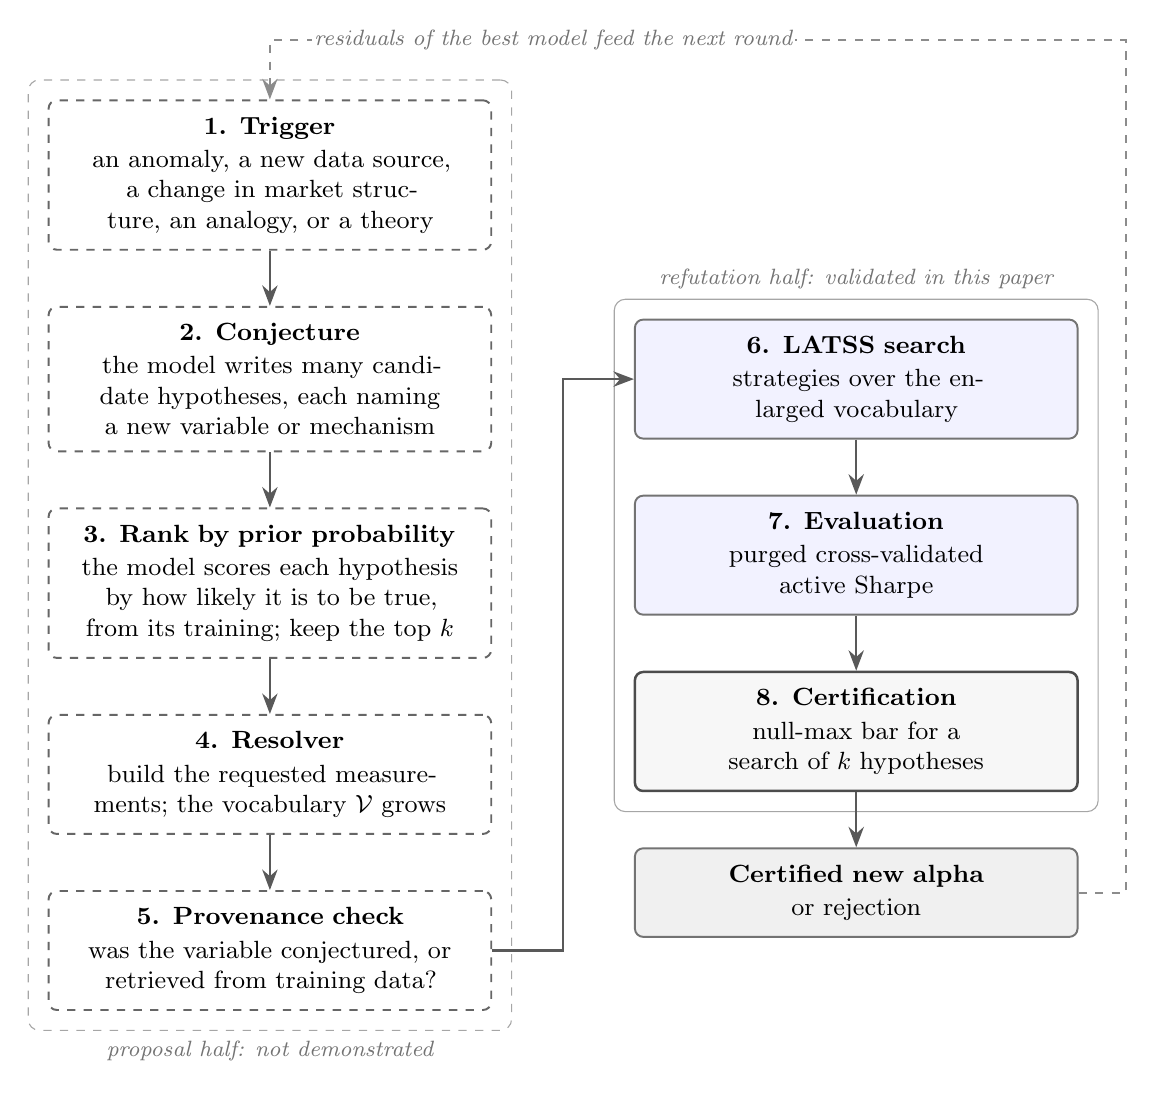
\begin{tikzpicture}[
  missing/.style={proc, text width=5.2cm, fill=white, dashed, draw=black!60},
  have/.style={proc, text width=5.2cm},
  node distance=7mm]
  \node[missing] (anom) {\textbf{1. Trigger}\\[1pt]an anomaly, a new data source, a change in market
    structure, an analogy, or a theory};
  \node[missing, below=of anom] (conj) {\textbf{2. Conjecture}\\[1pt]the model writes many candidate
    hypotheses, each naming a new variable or mechanism};
  \node[missing, below=of conj] (rank) {\textbf{3. Rank by prior probability}\\[1pt]the model scores
    each hypothesis by how likely it is to be true, from its training; keep the top $k$};
  \node[missing, below=of rank] (res) {\textbf{4. Resolver}\\[1pt]build the requested measurements;
    the vocabulary $\mathcal{V}$ grows};
  \node[missing, below=of res] (prov) {\textbf{5. Provenance check}\\[1pt]was the variable conjectured,
    or retrieved from training data?};
  \node[have, right=18mm of conj] (srch) {\textbf{6. LATSS search}\\[1pt]strategies over the enlarged
    vocabulary};
  \node[have, below=of srch] (cv) {\textbf{7. Evaluation}\\[1pt]purged cross-validated active Sharpe};
  \node[certnode, text width=5.2cm, below=of cv] (bar) {\textbf{8. Certification}\\[1pt]null-max bar
    for a search of $k$ hypotheses};
  \node[have, below=of bar, fill=black!6] (out) {\textbf{Certified new alpha}\\[1pt]or rejection};
  \draw[flow] (anom) -- (conj);
  \draw[flow] (conj) -- (rank);
  \draw[flow] (rank) -- (res);
  \draw[flow] (res) -- (prov);
  \draw[flow] (prov.east) -- ++(0.9,0) |- (srch.west);
  \draw[flow] (srch) -- (cv);
  \draw[flow] (cv) -- (bar);
  \draw[flow] (bar) -- (out);
  \draw[fb] (out.east) -- ++(0.6,0) |- ($(anom.north)+(0,0.75)$) -- (anom.north);
  \node[annot, align=center, fill=white, inner sep=1pt] at ($(anom.north)+(3.6,0.75)$)
    {residuals of the best model feed the next round};
  \begin{scope}[on background layer]
    \node[draw=black!35, dashed, rounded corners=4pt, inner sep=7pt,
      fit=(anom)(conj)(rank)(res)(prov), label={[annot]below:proposal half: not demonstrated}] {};
    \node[draw=black!35, rounded corners=4pt, inner sep=7pt,
      fit=(srch)(cv)(bar), label={[annot]above:refutation half: validated in this paper}] {};
  \end{scope}
\end{tikzpicture}
\caption{The conjectured invention loop. Steps 6 to 8 are the LATSS loop validated in
Sections~\ref{sec:method} to~\ref{sec:results}. Steps 1 to 5 (dashed) are the components the loop adds;
none has been demonstrated for economic variables. Steps 2 and 3 are where the language model works: it conjectures
hypotheses and ranks them by prior probability (Section~\ref{sec:prior}), and only the top $k$ go on to
be tested, so the bar in step 8 is the bar for a procedure that tests $k$ hypotheses.}
\label{fig:inventionloop}
\end{figure}

\paragraph{One round of the loop.} The steps of Figure~\ref{fig:inventionloop} are described in order,
with an illustration. The illustration is hypothetical; it shows what each step would do, not a result.

\begin{enumerate}[leftmargin=1.6em]
\item \textbf{Trigger.} Something has to tell the model what to explain or where to look. The
illustration uses an anomaly: after the search of step 6 has run on the current vocabulary, the returns of
the best strategy are examined for structure it leaves behind, for example losses that cluster in the
weeks after large customers of the held company report earnings. The anomaly is stated in words and passed
to the model as part of the prompt. An anomaly is not the only possible trigger; the alternatives are
listed after this walk-through.
\item \textbf{Conjecture.} The language model writes many candidate hypotheses that could explain the
anomaly, each of which names a variable that is not yet in the vocabulary. In the illustration these
might be: earnings news propagates from customers to suppliers with a delay; option-implied volatility
around customer announcements predicts the supplier's return; analyst forecast revisions for the
customer lead those for the supplier. Generation is cheap, so the model can write dozens or hundreds.
\item \textbf{Rank by prior probability.} The model then assigns each hypothesis a probability of being
true, based only on what it learned in training: the published evidence, the economic mechanism, and how
often similar effects have held up. The scores can be elicited directly (``give the probability that
this effect exists in U.S. large caps''), obtained by pairwise comparison, or read from the model's
likelihood of the hypothesis text (Section~\ref{sec:prior}). Only the $k$ highest-ranked hypotheses go
forward. This step must use no returns from the test history; the ranking is fixed before the data is
examined, so that it acts as a prior and not as a fit.
\item \textbf{Resolver.} Each of the $k$ hypotheses is turned into a measurement: the named variable is
built from an available data source and added to the vocabulary. A hypothesis that cannot be measured is
dropped here.
\item \textbf{Provenance check.} Before a result can count as invention, it must be established whether
the variable was conjectured or retrieved, that is, whether the model reproduced an effect it read about
in training. A retrieved effect can still be useful alpha, but it is not evidence of invention.
\item \textbf{LATSS search.} The validated loop runs over the enlarged vocabulary, proposing strategies
that use the new variables.
\item \textbf{Evaluation.} Each strategy is scored by purged cross-validated active Sharpe, exactly as in
Sections~\ref{sec:method} to~\ref{sec:results}.
\item \textbf{Certification.} The champion must clear the null-max bar computed for this procedure.
Because only $k$ hypotheses were tested, the bar is that of a procedure testing $k$ hypotheses, which we
expect, but have not measured, to be lower for small $k$ (Section~\ref{sec:prior}). If the champion clears, the
result is a certified strategy built on a new variable; if not, the residuals feed the next round.
\end{enumerate}

\paragraph{Triggers other than anomalies.} Peirce and Hanson describe inquiry as starting from a
surprising observation~\cite{peirce,hanson}, and in a loop that already has a best model, its residuals
are the natural source of surprise. Popper, by contrast, held that a conjecture may come from anywhere and
that only its test is governed by method~\cite{popper}. For alpha research at least five starting points
are in practical use, and each fits step 1 of the loop:
\begin{itemize}[leftmargin=1.4em]
\item \emph{An anomaly}: structure in the residuals of the current best strategy, as in the illustration.
\item \emph{A new data source}: a dataset becomes available, for example satellite counts of retail
parking lots or text of regulatory filings, and the question is what it could predict.
\item \emph{A change in market structure}: a new regulation, a change in index rules, the arrival of a new
class of participant, or a change in trading hours, each of which suggests who might now be forced to
trade at a predictable time.
\item \emph{An analogy}: an effect documented in one market, asset class, or field is conjectured to
exist in another.
\item \emph{A theory}: an economic mechanism, such as limits to arbitrage or slow diffusion of
information, is used to derive a prediction before any data is examined.
\end{itemize}
The trigger also matters for validity. Triggers that do not look at the test history, such as a new data
source, a structural change, an analogy, or a theory, keep the ranking of step 3 a genuine prior. An
anomaly found in the residuals of the test history uses that history once already, so a hypothesis it
suggests should be certified on data that the anomaly search did not see, or with a bar that includes the
anomaly search in the procedure it simulates.

Steps 2 and 3 together are the role of the language model in this loop: it supplies the hypotheses and
the prior probability of each. Section~\ref{sec:prior} gives the argument for why the ranking is
necessary and the condition under which it is valid; the walk-through shows where it sits. Steps 6 to 8
are the part this paper has validated. Steps 1, 4, and 5 are engineering and verification around the
model. Whether step 3 ranks true, uncrowded effects highly enough to be useful is the empirical question
on which the whole loop depends, and we found no measurement of it for economic hypotheses
(Section~\ref{sec:litreview}).

\paragraph{How many hypotheses to test.} The number $k$ passed from step 3 to the test is a trade-off
between two effects that pull in opposite directions. Testing more hypotheses raises the chance that a
true one is among them. It also raises the bar every hypothesis must clear, by analogy with E4, where the
bar rose with the number of candidates tried (Table~\ref{tab:capacity}); whether this reduces power for
new-variable hypotheses has not been measured. The best $k$ therefore depends on how good the ranking
is. If the ranking were uninformative, the order would not matter, and the loop would be a
blind search paying the full bar. If the ranking were perfect, $k=1$ would suffice. Between the two, the
value of the language model is measured by how far down its list a true effect typically sits, which is a
measurable property of the model and the domain.

\paragraph{Accounting across rounds.} The loop is iterative, and every round tests hypotheses on the same
history. A bar computed for the $k$ hypotheses of one round is valid for that round alone; after $r$
rounds, $rk$ hypotheses have been tested on the same data, and the bar must reflect the whole procedure,
including the anomaly searches that triggered later rounds. Without that accounting the loop becomes the
process Novy-Marx and Velikov describe, mining many signals and supplying a story for each
afterward~\cite{novymarx}. Two remedies are available. The bar can be recomputed by simulating the entire
multi-round procedure on scrambled data, which follows directly from the same-class condition of
Section~\ref{sec:bar}. Or the rounds can be combined in a sequential test whose false-positive rate
holds no matter when testing stops; POPPER does this for hypothesis validation with language models by
multiplying e-values, a measure of evidence that can be combined across experiments without losing error control,~\cite{falsify}.

\paragraph{Ways the ranking can fail.} The ranking of step 3 is learned from text, and three features of
that text work against it in finance. First, the model's prior favors what is most often written about,
and in markets the effects most written about are the ones most traded: McLean and Pontiff found that the
returns of published predictors fall substantially after publication~\cite{mcleanpontiff}. A ranking that
puts well-documented effects first may put the most arbitraged effects first. Second, the model may know
the answer: if an effect and its replication record appear in the training data, a high rank reflects
memory of a result, not a prediction, which is why step 5 exists. Third, published finance research
over-represents positive results~\cite{harvey}, so the training text overstates how often plausible-sounding effects
hold. Each of these failures would show up as poor calibration: hypotheses ranked high would replicate no
more often than hypotheses ranked low.

\paragraph{How the ranking could be measured.} Calibration can be tested before any of the loop is built.
Take predictors whose fate after the model's training cutoff is known, for example effects published, or
data sources released, after that date. Ask the model to rank them without seeing any results, then check
whether the higher-ranked ones performed better in the later data. This is the temporal split that Qi et
al.\ use for biomedical hypotheses~\cite{qi2023}, applied to economic ones. A ranking that tracks later
performance supports step 3; a flat or inverted relationship would mean the model's prior does not help,
and that the loop's proposal stage reduces to blind search.

\paragraph{What success would and would not show.} If the loop certifies a strategy built on a variable
the model proposed, the result is a certified candidate for economic novelty: a source of return not
previously in the strategy's inputs, which still requires forward testing after costs and crowding to
reach the economic level of Table~\ref{tab:novelty}. Whether it is also invention depends on step 5. If the
variable or the effect appears in the model's training material, the loop has retrieved and tested a
known idea, which is useful but is the selective abduction of Section~\ref{sec:litreview}. Only a variable
that the provenance check shows was absent from the training material would count as creative abduction,
the step for which no machine demonstration exists. The loop can therefore succeed at producing alpha
without settling the question of invention, and the two outcomes should be reported separately.

\paragraph{The human in the current loop.} In practice today, steps 1, 4, and 5 are done by people. A
researcher notices the anomaly or the new data source, builds the requested measurement, and judges
whether the idea was new. The language model contributes steps 2 and 3, and LATSS contributes steps 6 to
8. The research program implied by Figure~\ref{fig:inventionloop} is to automate the remaining steps one
at a time, measuring at each stage whether the loop's certified output improves, and the benchmark of
Section~\ref{sec:jumpbench} is the proposed way to measure the hardest of them.

\begin{table}[htbp]
\centering
\caption{Component-by-component gap between the search loop validated in this paper and the invention
loop it suggests.}
\label{tab:gaps}
\small
\begin{tabular}{p{2.6cm} p{3.9cm} p{3.9cm} p{3.6cm}}
\toprule
Component & Validated search loop & Invention loop & Gap \\
\midrule
Hypothesis space & Fixed feature vocabulary supplied by a human & Must grow at run time: the agent
requests measurements that were never supplied & The request tool and resolver exist only in the proposed
benchmark (Section~\ref{sec:jumpbench}) \\
\addlinespace
Proposal step & Mutate formulas over the given features, by model or by grammar & Conjecture many
hypotheses naming new variables, rank them by prior probability, test the top $k$ & Ranking of representable hypotheses is possible in principle, accuracy unmeasured (Section~\ref{sec:prior});
generation outside the reachable set does not, and the prior points at crowded, known ideas \\
\addlinespace
Trigger & None; the search runs unconditionally & An anomaly in the residuals, a new data source, a
change in market structure, an analogy, or a theory & The loop does not yet surface residuals or other
triggers as prompts \\
\addlinespace
Evaluation & Backtest with purged cross-validation & Unchanged & None; carries over as validated (E1,
E3) \\
\addlinespace
Certification & Same-class null-max bar & The same bar, recomputed over the enlarged class after each
accepted feature, plus a jump rate against a base rate & Bar recomputation is defined
(Section~\ref{sec:bar}); the jump metric is proposed, not built \\
\addlinespace
Validation of the loop itself & Power curve on a dialed synthetic signal & Jump rate with a human
positive control & Benchmark unbuilt; no measurement exists \\
\addlinespace
Provenance & Not required & Must rule out that the named variable was retrieved from training data
rather than conjectured & Unsolved \\
\bottomrule
\end{tabular}
\end{table}

The refutation half of the loop, evaluation and certification, is validated on the synthetic test-bed;
every open gap is in the proposal half: the trigger, the conjecture of a new variable, its ranking, and
the means of verifying that a conjecture was not retrieved from training data.

\subsection{Alpha discovery as an inverse problem}
\label{sec:inverse}

The division of labor above has a counterpart in inverse-problem theory, a mature field in the physical
sciences, and the language-model inverse-problem solvers of that field are the closest precedent for
LATSS outside finance.

\paragraph{The forward and the inverse problem.} A forward problem maps a model, its parameters and
structure, to observable consequences, and is usually well-posed: the output exists, is unique, and
varies continuously with the input. The inverse problem runs the other way, inferring the model from
observations, and is generically ill-posed in Hadamard's sense: a solution may fail to exist, may not be
unique, and may be unstable, so that a small change in the data forces a large change in the inferred
model. Measurement noise sharpens all three difficulties. The classical responses are regularization and
prior information, which restrict or weight the model space so that the inference becomes tractable.
Figure~\ref{fig:forwardinverse} draws the two directions for the trading case.

\begin{figure}[htbp]
\centering
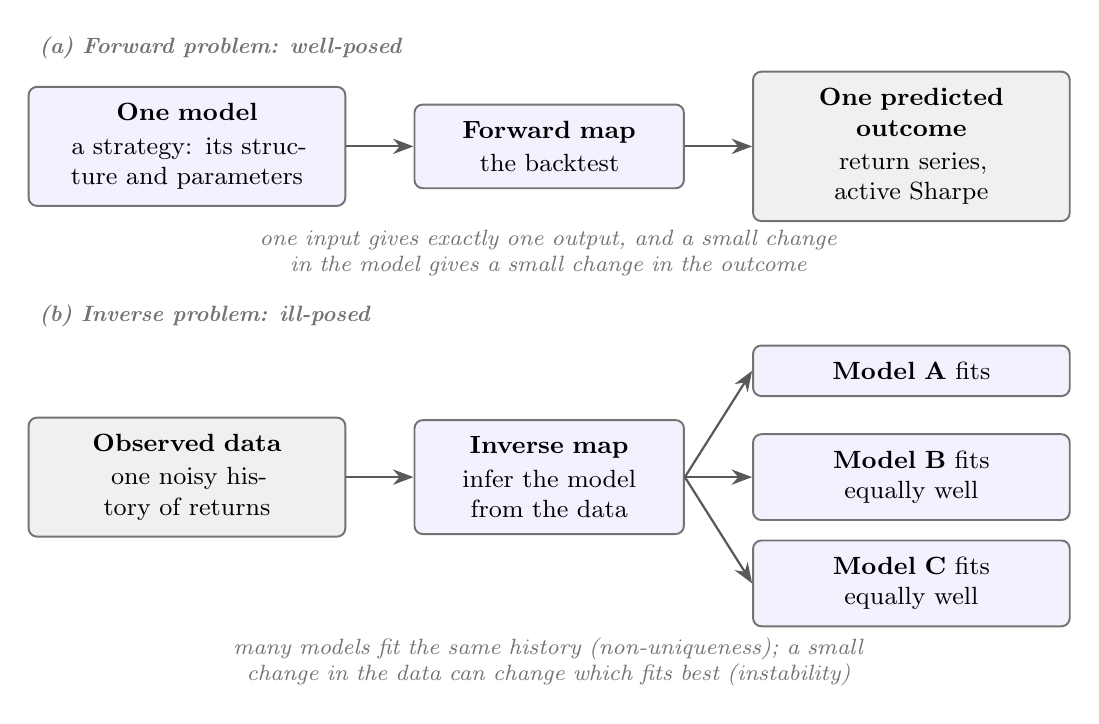
\begin{tikzpicture}[
  box/.style={proc, text width=3.6cm},
  obs/.style={proc, text width=3.6cm, fill=black!6},
  node distance=6mm]
  % (a) forward problem
  \node[annot, anchor=west] at (-0.6,1.25) {\textbf{(a) Forward problem: well-posed}};
  \node[box] (fm) at (1.4,0) {\textbf{One model}\\[1pt]a strategy: its structure and parameters};
  \node[proc, text width=3.0cm] (fg) at (6.0,0) {\textbf{Forward map}\\[1pt]the backtest};
  \node[obs] (fd) at (10.6,0) {\textbf{One predicted outcome}\\[1pt]return series, active Sharpe};
  \draw[flow] (fm) -- (fg);
  \draw[flow] (fg) -- (fd);
  \node[annot, align=center, text width=11cm] at (6.0,-1.35) {one input gives exactly one output, and a
  small change in the model gives a small change in the outcome};
  % (b) inverse problem
  \node[annot, anchor=west] at (-0.6,-2.15) {\textbf{(b) Inverse problem: ill-posed}};
  \node[obs] (id) at (1.4,-4.2) {\textbf{Observed data}\\[1pt]one noisy history of returns};
  \node[box] (m1) at (10.6,-2.85) {\textbf{Model A} fits};
  \node[box] (m2) at (10.6,-4.2) {\textbf{Model B} fits equally well};
  \node[box] (m3) at (10.6,-5.55) {\textbf{Model C} fits equally well};
  \node[proc, text width=3.0cm] (ig) at (6.0,-4.2) {\textbf{Inverse map}\\[1pt]infer the model from the data};
  \draw[flow] (id) -- (ig);
  \draw[flow] (ig.east) -- (m1.west);
  \draw[flow] (ig.east) -- (m2.west);
  \draw[flow] (ig.east) -- (m3.west);
  \node[annot, align=center, text width=11cm] at (6.0,-6.55) {many models fit the same history
  (non-uniqueness); a small change in the data can change which fits best (instability)};
\end{tikzpicture}
\caption{The forward and inverse problems for a trading strategy. (a) Running a known strategy through the
backtest gives one outcome. (b) Inferring the strategy from one noisy history admits many equally good
fits. Figure~\ref{fig:tarantola} draws Tarantola's response.}
\label{fig:forwardinverse}
\end{figure}

\paragraph{Popper, Bayes, and Tarantola.} The oldest tradition, from Gauss and Legendre, and from
Boscovich and Laplace for least absolute values, casts the
inverse problem as optimization and seeks the single best-fit model, least squares being the criterion
that follows from assuming Gaussian measurement errors~\cite{tarantola_np}. Tarantola argues this is the
wrong object. Observations, he writes, cannot produce models, they can only falsify them, so displaying
one best model lends it a veracity its uncertainties do not warrant, and in a high-dimensional model
space the posterior is typically multimodal, with whole subspaces of equivalent fits, so optimization to
a point is not even well defined. His prescription is explicitly both Bayesian and Popperian: use all
available prior information to generate models of the system, potentially without limit; for each, solve
the forward problem, compare its predictions with the observations, and drop the models the comparison
falsifies; the collection that survives is the solution~\cite{tarantola_np,tarantola_book}. Passing from
this prior collection of models to the surviving posterior collection is the Bayesian content, and the
keep-or-drop test on each model is the Popperian content. Prior information is structural rather than
optional, because the problem is underdetermined and the space of models is so large
that even finding one consistent model is hard. Figure~\ref{fig:tarantola} draws the prescription.

\begin{figure}[htbp]
\centering
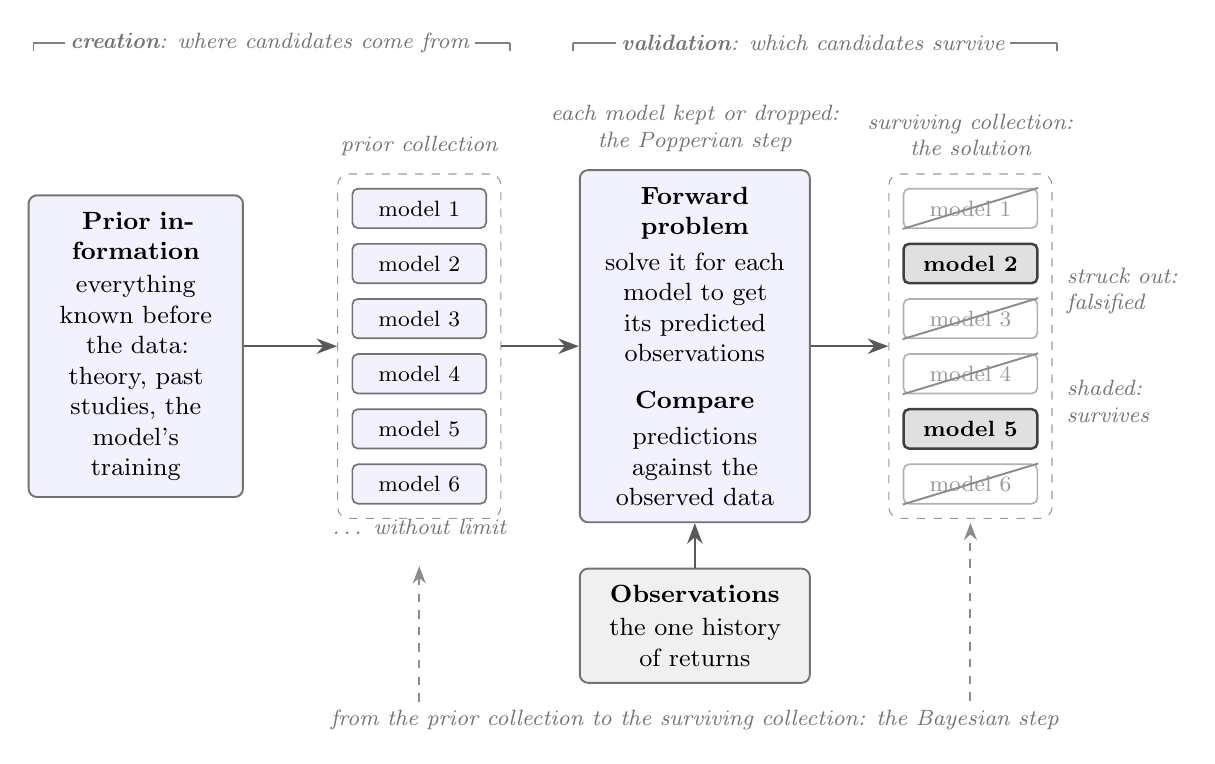
\begin{tikzpicture}[
  mdl/.style={rectangle, rounded corners=2pt, draw=black!55, line width=0.6pt, fill=blue!5,
    minimum width=1.7cm, minimum height=0.5cm, font=\footnotesize},
  dead/.style={mdl, fill=white, draw=black!30, text=black!40},
  live/.style={mdl, fill=black!12, draw=black!75, line width=0.9pt, font=\footnotesize\bfseries}]
  % prior information
  \node[proc, text width=2.3cm] (pi) at (0,0) {\textbf{Prior information}\\[1pt]everything known
    before the data: theory, past studies, the model's training};
  % prior collection
  \foreach \i/\y in {1/1.75, 2/1.05, 3/0.35, 4/-0.35, 5/-1.05, 6/-1.75}
    \node[mdl] (a\i) at (3.6,\y) {model \i};
  \node[annot] at (3.6,-2.3) {\dots\ without limit};
  \node[draw=black!40, dashed, rounded corners=4pt, inner sep=5pt, fit=(a1)(a6)] (prior) {};
  \node[annot, align=center, above=1mm of prior] {prior collection};
  % forward problem and comparison
  \node[proc, text width=2.5cm, minimum height=4.3cm] (cmp) at (7.1,0) {\textbf{Forward problem}\\[2pt]
    solve it for each model to get its predicted observations\\[6pt]\textbf{Compare}\\[2pt]predictions
    against the observed data};
  \node[proc, text width=2.5cm, fill=black!6] (obs) at (7.1,-3.55) {\textbf{Observations}\\[1pt]the one
    history of returns};
  \draw[flow] (obs) -- (cmp);
  \node[annot, align=center, above=1mm of cmp] {each model kept or dropped:\\ the Popperian step};
  % posterior collection
  \node[dead] (b1) at (10.6,1.75) {model 1};
  \node[live] (b2) at (10.6,1.05) {model 2};
  \node[dead] (b3) at (10.6,0.35) {model 3};
  \node[dead] (b4) at (10.6,-0.35) {model 4};
  \node[live] (b5) at (10.6,-1.05) {model 5};
  \node[dead] (b6) at (10.6,-1.75) {model 6};
  \foreach \i in {1,3,4,6}
    \draw[black!45, line width=0.7pt] (b\i.south west) -- (b\i.north east);
  \node[draw=black!40, dashed, rounded corners=4pt, inner sep=5pt, fit=(b1)(b6)] (post) {};
  \node[annot, align=center, above=1mm of post] {surviving collection:\\ the solution};
  \node[annot, align=left, anchor=west] at (11.7,0.7) {struck out:\\ falsified};
  \node[annot, align=left, anchor=west] at (11.7,-0.7) {shaded:\\ survives};
  % creation vs validation
  \draw[black!50, line width=0.6pt] (-1.3,3.85) -- (4.75,3.85);
  \draw[black!50, line width=0.6pt] (-1.3,3.75) -- (-1.3,3.85);
  \draw[black!50, line width=0.6pt] (4.75,3.75) -- (4.75,3.85);
  \node[annot, fill=white, inner sep=2pt] at (1.7,3.85) {\textbf{creation}: where candidates come from};
  \draw[black!50, line width=0.6pt] (5.55,3.85) -- (11.7,3.85);
  \draw[black!50, line width=0.6pt] (5.55,3.75) -- (5.55,3.85);
  \draw[black!50, line width=0.6pt] (11.7,3.75) -- (11.7,3.85);
  \node[annot, fill=white, inner sep=2pt] at (8.6,3.85) {\textbf{validation}: which candidates survive};
  % flows
  \draw[flow] (pi) -- (prior);
  \draw[flow] (prior) -- (cmp);
  \draw[flow] (cmp) -- (post);
  % Bayesian content
  \draw[fb, {Stealth[length=2.2mm]}-{Stealth[length=2.2mm]}] ($(prior.south)+(0,-0.6)$) |- (7.1,-4.75)
    -| ($(post.south)+(0,-0.05)$);
  \node[annot, align=center, fill=white, inner sep=2pt] at (7.1,-4.75) {from the prior collection to the
    surviving collection: the Bayesian step};
\end{tikzpicture}
\caption{Tarantola's prescription for the inverse problem. Prior information generates a collection of
candidate models, without a fixed limit on how many. The forward problem is solved for each model and its
predictions are compared with the observed data; each model is kept or dropped on that comparison, which
is the Popperian step. The collection that survives is the solution, and the passage from the prior
collection to the surviving one is the Bayesian step. In LATSS the language model supplies the candidates,
the backtest is the forward problem, and cross-validation with the null-max bar is the comparison. The
left half is the creation of candidate models; the right half is their validation. Tarantola's procedure
specifies the validation and takes the prior as given.}
\label{fig:tarantola}
\end{figure}

\paragraph{The mapping to alpha search.} Each element of Tarantola's procedure has a concrete
counterpart in LATSS, listed in Table~\ref{tab:tarantolamap} and explained below.

\begin{table}[htbp]
\centering
\caption{Tarantola's inverse-problem procedure and its counterpart in LATSS.}
\label{tab:tarantolamap}
\small
\begin{tabular}{p{3.0cm} p{6.4cm} p{4.4cm}}
\toprule
Tarantola & LATSS & Where in this paper \\
\midrule
Model & A strategy: a scoring function together with its fitted parameters & Section~\ref{sec:loop} \\
Observations & One history of daily returns for the seven names, 2{,}952 trading days &
Section~\ref{sec:method} \\
Forward problem & The backtest: run the strategy over the history and compute its active Sharpe &
Eq.~\eqref{eq:activesharpe} \\
Prior information & The feature vocabulary chosen by a human, the representation (Python functions), and the
language model's proposal distribution & Eq.~\eqref{eq:proposal} \\
Noise model & The distribution of best scores the same search achieves on sign-flipped returns &
Section~\ref{sec:bar} \\
Falsification & A candidate is dropped unless its cross-validated score exceeds the null-max bar &
Section~\ref{sec:bar} \\
Solution & The collection of candidates that survive the bar & This subsection \\
\bottomrule
\end{tabular}
\end{table}

\emph{The forward problem.} The backtest is a deterministic calculation with no modeling error of its
own, unlike the forward problems of geophysics, so all of the difficulty lies in the data: one history,
against which every candidate is judged. With about 11.7 years of returns, the standard error of an
annualized Sharpe ratio near zero is roughly $1/\sqrt{11.7}\approx 0.29$, so two strategies whose true
Sharpe ratios differ by 0.3 can easily swap order on this history.

\emph{Why the inverse problem is ill-posed here.} Each of Hadamard's three failures appears in our
experiments. Existence fails when the true driver is not expressible in the vocabulary, as in E12a
(Section~\ref{sec:e12a}). Uniqueness fails because many strategies fit the same history: in E2
(Section~\ref{sec:e2}) champions exceed the oracle by fitting the noise features on top of the real one.
Stability fails because a small change in the data changes the answer: replacing only the noise in the
features with a new realization moves the oracle active Sharpe at $\rho=0.20$ by a standard deviation of
0.30 across 30 realizations (from 0.83 on average to 0.95 for the realization E1 searched,
Table~\ref{tab:power}). Overfitting, in this language, is the non-uniqueness of the inverse problem
mistaken for a solution.

\emph{The prior.} Tarantola's prior is a probability distribution that can be evaluated for any model.
The LATSS prior, the vocabulary, the representation, and the proposal distribution of
Eq.~\eqref{eq:proposal}, is available only by sampling, unless the model is asked for an explicit
plausibility, which is the step Section~\ref{sec:prior} adds.

\emph{The noise model and the falsification step.} Tarantola drops a model when its predictions are
improbable under the noise model. LATSS has no analytic noise model for returns, so it builds one by
simulation from sign-flipped returns. This step contains a correction that a model-by-model test does
not: LATSS keeps the best of many candidates, and the best of many noise fits is higher than any single
one, so the bar is built from the maximum over the whole search, which is why it must be computed over
the same search that produced the candidates (Section~\ref{sec:bar}).

\emph{The solution.} In Tarantola's account the solution is the collection of models that survive, not a
single best model, because in an ill-posed problem the best fit is not identified. The faithful output of
LATSS is therefore every candidate whose score exceeds the bar. Our experiments report only whether the
champion clears the bar; reporting the full surviving collection is a direct extension. Certification in
either form means only that a strategy has not been falsified by this test on this history.

\emph{Creation and validation.} The two halves of Figure~\ref{fig:tarantola} set two separate
requirements for new alpha: some candidate in the prior collection must contain the true mechanism
(creation), and that candidate must survive the comparison (validation). A perfect validator cannot
produce new alpha from a prior that does not contain it, and a rich prior is worthless if the validator
certifies noise.

The two loops of this paper fill the left half differently. In the search loop validated in
Sections~\ref{sec:method} to~\ref{sec:results}, creation is limited to new strategies over a fixed
vocabulary: the language model writes scoring functions that combine features a human supplied. In the
invention loop of Figure~\ref{fig:inventionloop}, creation reaches one level further, to new variables.
The procedure then runs twice, one inside the other. At the outer level the candidate models are
hypotheses about which variables matter, and the language model's ranking is the prior probability over
them. At the inner level, for each accepted hypothesis, the candidate models are strategies built on the
enlarged vocabulary, and LATSS validates them. Table~\ref{tab:fig9tarantola} maps each step of
Figure~\ref{fig:inventionloop} to its role in Tarantola's procedure.

\begin{table}[htbp]
\centering
\caption{The steps of the invention loop (Figure~\ref{fig:inventionloop}) and their role in Tarantola's
procedure (Figure~\ref{fig:tarantola}).}
\label{tab:fig9tarantola}
\small
\begin{tabular}{>{\raggedright\arraybackslash}p{3.2cm} >{\raggedright\arraybackslash}p{5.0cm}
>{\raggedright\arraybackslash}p{2.0cm} >{\raggedright\arraybackslash}p{3.4cm}}
\toprule
Step of Figure~\ref{fig:inventionloop} & Role in Tarantola's procedure & Half & Status \\
\midrule
1. Trigger & The prior information that prompts a new round: an anomaly, a data source, a structural
change, an analogy, or a theory & Creation & Done by people today \\
\addlinespace
2. Conjecture & Generate the prior collection at the outer level: candidate hypotheses naming new
variables & Creation & Language model; quality unmeasured \\
\addlinespace
3. Rank by prior probability & Assign prior probabilities to the collection and keep the most probable
$k$ & Creation & Language model; calibration unmeasured \\
\addlinespace
4. Resolver & Make each hypothesis computable, so that its forward problem can be solved & Bridge &
Done by people today \\
\addlinespace
5. Provenance check & No counterpart; it concerns whether the idea was new, not whether it is true &
Neither & Unsolved \\
\addlinespace
6. LATSS search & Generate the prior collection at the inner level: strategies over the enlarged
vocabulary & Creation & Validated in this paper \\
\addlinespace
7. Evaluation & Solve the forward problem for each strategy: the backtest & Validation & Validated in
this paper \\
\addlinespace
8. Certification & Compare with the observations and drop what is falsified: the null-max bar for $k$
hypotheses & Validation & Validated in this paper \\
\addlinespace
Certified new alpha & The surviving collection & Result & Not yet produced by the full loop \\
\bottomrule
\end{tabular}
\end{table}

The table shows where the paper's results sit. Everything this paper has measured is validation, plus
creation at the inner level, over a vocabulary a human chose. Creation at the outer level, the
conjecture and ranking of new variables, is the part that would turn validated search into the
production of new alpha, and we found no measurement of it.

\paragraph{Solving inverse problems with language models.} Outside finance, the inverse problem has a
long-studied special case called \emph{symbolic regression}: given measurements of a physical or
biological system, find a closed-form equation that reproduces them, for example recovering
$F = m a$ from recorded forces, masses, and accelerations. Classical symbolic regression searches
over expression trees by genetic programming (Section~\ref{sec:related}). Since 2024 several systems
have replaced the hand-built mutation step with a language model, and they have the same shape as LATSS.
Two are representative.

\emph{LLM-SR} (Large Language Model-based Symbolic Regression) treats an equation as a short Python
program~\cite{llmsr}. The language model proposes an equation skeleton, the form of the equation with its
numeric constants left as free parameters, drawing on what it knows about the scientific domain. An
optimizer fits the constants to the data, the fitted equation is scored by how well it reproduces the
measurements, and the best skeletons with their scores are fed back into the next prompt. The authors
test it on physics and biology problems built so that the model cannot simply recite a known equation.

\emph{SGA} (Scientific Generative Agent) splits the problem into two levels~\cite{sga}. At the upper
level the language model proposes the discrete part of a hypothesis, such as the form of a physical law
for how a material deforms, or a molecular structure. At the lower level a differentiable physics
simulation runs the hypothesis and adjusts its continuous parameters by gradient descent to match the
observations. The loss after fitting is returned to the language model, which proposes the next
hypothesis. It was evaluated on discovering constitutive laws of materials and on molecular design. A
benchmark, LLM-SRBench, now compares systems of this kind on equation discovery~\cite{llmsrbench}.

Figure~\ref{fig:llminverse} draws the common loop, and Table~\ref{tab:llminverse} maps each of its steps
to LLM-SR, SGA, and LATSS.

\begin{figure}[htbp]
\centering
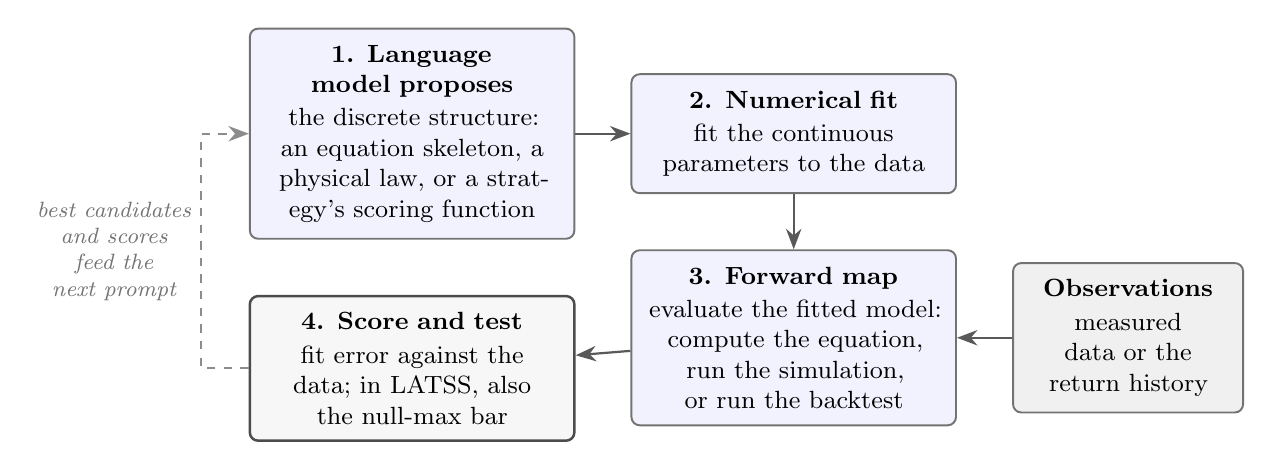
\begin{tikzpicture}[node distance=7mm and 7mm]
  \node[proc, text width=3.7cm] (prop) {\textbf{1. Language model proposes}\\[1pt]the discrete structure:
    an equation skeleton, a physical law, or a strategy's scoring function};
  \node[proc, text width=3.7cm, right=of prop] (fit) {\textbf{2. Numerical fit}\\[1pt]fit the
    continuous parameters to the data};
  \node[proc, text width=3.7cm, below=of fit] (fwd) {\textbf{3. Forward map}\\[1pt]evaluate the fitted
    model: compute the equation, run the simulation, or run the backtest};
  \node[certnode, text width=3.7cm, below=of prop] (score) {\textbf{4. Score and test}\\[1pt]fit error
    against the data; in LATSS, also the null-max bar};
  \node[proc, text width=2.5cm, fill=black!6, right=of fwd] (obs) {\textbf{Observations}\\[1pt]measured
    data or the return history};
  \draw[flow] (prop) -- (fit);
  \draw[flow] (fit) -- (fwd);
  \draw[flow] (fwd) -- (score);
  \draw[flow] (obs) -- (fwd);
  \draw[fb] (score.west) -- ++(-0.6,0) |- (prop.west)
    node[annot, pos=0.25, left, align=center] {best candidates\\ and scores\\ feed the\\ next prompt};
\end{tikzpicture}
\caption{The common loop of language-model inverse-problem solvers. The language model proposes structure,
a numerical method fits parameters, the forward map evaluates the fitted model against the observations,
and the scores return to the model. LLM-SR, SGA, and LATSS differ in the domain and in step 4: LATSS adds a
test calibrated against what the same search achieves on data with no signal.}
\label{fig:llminverse}
\end{figure}

\begin{table}[htbp]
\centering
\caption{Steps of the loop in Figure~\ref{fig:llminverse} in three systems.}
\label{tab:llminverse}
\small
\begin{tabular}{>{\raggedright\arraybackslash}p{2.9cm} >{\raggedright\arraybackslash}p{3.6cm} >{\raggedright\arraybackslash}p{3.6cm} >{\raggedright\arraybackslash}p{3.6cm}}
\toprule
Step & LLM-SR~\cite{llmsr} & SGA~\cite{sga} & LATSS \\
\midrule
Observations & Measurements of a physical or biological system & Measured behavior of a material or
molecule & One history of daily stock returns \\
\addlinespace
Structure the model proposes & Equation skeleton as a Python program & Form of a physical law or a
molecular structure & Scoring function as a Python program \\
\addlinespace
Numerical fit & Optimizer fits the equation's constants & Gradient descent through a differentiable
simulation & Differential evolution fits the strategy's parameters \\
\addlinespace
Forward map & Evaluate the equation on the inputs & Run the simulation & Run the backtest \\
\addlinespace
Score & Error between equation and data & Loss between simulation and data & Cross-validated active
Sharpe \\
\addlinespace
Test against chance fits & Not part of the method as described & Not part of the method as described &
Same-class null-max bar \\
\addlinespace
Supplied building blocks & Input variables and allowed operations & Simulator and the components it
accepts & Feature vocabulary and Python operations \\
\bottomrule
\end{tabular}
\end{table}

Three points follow from the mapping. First, the architecture is shared. A language model that proposes
structure, a numerical layer that fits parameters, and a forward map that scores the result is the
general form of a language-model inverse-problem solver, and LATSS is that form applied to trading
strategies. Second, the domains differ in how much noise surrounds the signal, and that changes which
step matters most. A physical law fitted to laboratory measurements either reproduces them closely or
does not, so the fit error is an informative score. A trading strategy fitted to one history of returns
can score well by fitting noise alone, as E3 shows, so a test calibrated against chance fits is
indispensable in finance and is the step LATSS adds. Third, the limit is shared. Each system searches
the structures that can be built from its supplied building blocks. SGA reports solutions that differ
from conventional expectations, which is novelty at the solution level of Table~\ref{tab:novelty}; none
of these systems is reported to have introduced a variable or concept outside its supplied building
blocks. Progress on language-model inverse-problem solving is therefore progress on search and testing
within a supplied space, which is the capability LATSS validates and the boundary the benchmark below
probes.

\emph{Mapping to the invention loop.} Table~\ref{tab:llminverse} compares the three systems as search
loops. The same systems can be placed on the invention loop of Figure~\ref{fig:inventionloop}, which
shows which of its steps they perform and which they leave out (Table~\ref{tab:llminverseinv}). All three
perform the inner level: they propose structures built from inputs that a person supplied, fit their
parameters, and score them against data (steps 6 and 7). None performs the outer level. None starts from
a trigger it identifies itself, none proposes a new input variable, and none ranks hypotheses by prior
probability before testing; they rank by fit after testing. The variables of LLM-SR and the components of
SGA's simulator are given in advance, so the resolver and provenance steps do not arise. LATSS differs
from the other two only at step 8, where it adds a test calibrated against chance fits.

\begin{table}[htbp]
\centering
\caption{Steps of the invention loop (Figure~\ref{fig:inventionloop}) performed by language-model
inverse-problem solvers and by LATSS as validated in this paper.}
\label{tab:llminverseinv}
\small
\begin{tabular}{>{\raggedright\arraybackslash}p{3.6cm} >{\raggedright\arraybackslash}p{3.2cm}
>{\raggedright\arraybackslash}p{3.2cm} >{\raggedright\arraybackslash}p{3.2cm}}
\toprule
Step of Figure~\ref{fig:inventionloop} & LLM-SR~\cite{llmsr} & SGA~\cite{sga} & LATSS (this paper) \\
\midrule
1. Trigger & No; the problem and data are given & No; the task is given & No; the vocabulary is given \\
2. Conjecture new variables & No; proposes equation forms over given variables & No; proposes laws or
structures over given components & No; proposes strategies over given features \\
3. Rank by prior probability & No; ranks by fit & No; ranks by loss & No; ranks by cross-validated score \\
4. Resolver & Not needed & Not needed & Not needed \\
5. Provenance check & No & No & No \\
6. Search over structures & Yes & Yes & Yes \\
7. Evaluation & Yes, fit error & Yes, simulation loss & Yes, cross-validated active Sharpe \\
8. Test against chance fits & No & No & Yes, null-max bar \\
\bottomrule
\end{tabular}
\end{table}

Two consequences follow for alpha invention. First, the success of these systems in science is evidence
about the inner level only: a language model can propose good structures over variables it is given,
including on problems built so that the answer cannot simply be recalled. That supports step 6 of the
invention loop and says nothing about steps 2 and 3. Second, the step LATSS adds is the one finance
needs most and the sciences need least. In a laboratory setting a wrong law fits the data badly; in a
single return history a wrong strategy can fit well by chance, so the inner level of an alpha-invention
loop must carry the calibrated test of step 8 regardless of how good its proposals are. The outer level,
proposing and ranking new variables, remains open in all three domains.

\subsection{A benchmark for hypothesis invention}
\label{sec:jumpbench}

Of the directions in this section, the benchmark matters most to the argument. It is the single
experiment that converts the question of machine invention from a debate into a measured quantity, and
the only one whose outcome could overturn the paper's claim about invention, so we set it out in detail. The
requirement is a way to score the jump, and we propose the following protocol, of which
Section~\ref{sec:e12a} is a first component.

The protocol reuses the test-bed machinery of this paper, the synthetic panel, the dialed signal
strength, and the same-class bar, but it inverts the question. In E1 the predictive feature is supplied
to the searcher and the measured quantity is the power of the search; here the true driver is withheld
from the vocabulary and the measured quantity is whether the agent asks for it. The scored action is
not combining given features into a strategy but requesting, in natural language, a measurement that
was never supplied.

\begin{enumerate}[leftmargin=1.6em]
\item \textbf{World.} Construct a synthetic panel whose true driver $V$ is a \emph{nameable} quantity
that is absent from the supplied vocabulary, for example a calendar or turn-of-month seasonal, an
exogenous named series, or a regime-conditional interaction of two features. Signal strength is tunable
as in Eq.~\eqref{eq:synth}, so power can be mapped against it.
\item \textbf{Vocabulary and request tool.} The agent receives a feature set that excludes $V$, together
with a tool for requesting a new measurement or data source described in natural language.
\item \textbf{Interface.} Each round the agent either proposes a strategy over current features (search)
or proposes a new measurement by description (a candidate jump). A resolver instantiates a requested
measurement when it matches an allowed library, in which $V$ is instantiable once named.
\item \textbf{Resolver and metric.} An automated judge, with human adjudication, maps a natural-language
request to whether it denotes $V$ or a sufficient statistic of it. The primary metric is the
\emph{jump rate}, the fraction of worlds in which the agent names $V$ without a hint, measured against a
base rate estimated from a fixed menu of generic requests (momentum, volatility, volume, and the like).
\item \textbf{Positive control.} Human experts, or an oracle with domain access, attempt the same task;
the jump must be achievable for them at a rate well above the base rate, or the world is ill-posed and
is discarded.
\item \textbf{Certification.} A named-and-instantiated $V$ must still yield a strategy that clears the
same-class null-max bar (Section~\ref{sec:bar}), so a jump counts only when it is both proposed and
certified.
\end{enumerate}

As a worked example, let $V$ be a day-of-week or turn-of-month seasonal while the supplied features are
price-only technicals with no calendar input. The agent must conjecture that returns depend on the
calendar and request a calendar feature; the base-rate menu never includes it. Mechanical searchers
cannot propose at all and score zero by construction, which is the point: this experiment is about the
conjecture step, not the search step. Calendar effects are textbook material, so naming one is retrieval,
and this example measures the second answer of the introduction, the ability to propose a known kind of
variable that the vocabulary lacks. A test of invention in the strong sense needs a driver with no
precedent in any text the model could have read, for example a synthetic mechanism defined only by the
benchmark, together with the provenance check. Related efforts give templates for the machinery, including
benchmarks that control an agent's prior knowledge in interactive discovery~\cite{physgym} and agentic
loops that automate sequential falsification of proposed hypotheses~\cite{falsify}.

\paragraph{Criteria for progress.} A system shows progress when its jump rate is
significantly above the base rate, with provenance showing $V$ was neither hinted nor inferable from
the supplied features, certified by the bar, across many worlds and seeds. Such a result would be the
first evidence against the ceiling of Section~\ref{sec:ceiling}, and it is exactly the falsification
condition stated there.

\paragraph{The design space.} The benchmark is a family of tasks, not a single one, graded by how far
the true driver sits from the supplied vocabulary. The easiest worlds hide a driver one short
description away, such as a calendar effect absent from price-only features; harder worlds require an
exogenous series the agent must think to pull in, or a regime-conditional interaction that only a
structural hypothesis would suggest; the hardest place the driver in a relation no generic menu covers.
Three arms make the comparison informative: a mechanical searcher that cannot propose and sets the
floor at zero, a base-rate arm that proposes from a fixed generic menu, and the system under test. The
human positive control sets the ceiling and certifies that each world is solvable, so the jump rate is
read between a floor that is zero by construction and a ceiling a person can reach.

\paragraph{Role of the benchmark.} The test is deliberately not about trading. Its subject is
whether an agent can conjecture a variable outside the space it was given, with alpha as one instance, so
a benchmark that works here transfers to scientific discovery more broadly, and the controlled-prior and
sequential-falsification systems already in the literature~\cite{physgym,falsify} supply much of the
machinery. It also inherits the discipline of this paper: a proposal counts only when it is named, with
provenance ruling out retrieval, and certified by a same-class bar, so the benchmark cannot be gamed by
fluent but unfalsifiable suggestions. For these reasons we regard it as the most valuable single piece of
future work the paper points to, and the natural next build on top of the certification layer established
here.

\subsection{Strengthening the measurement tool}
\label{sec:future}

These do not discover alpha, but they are prerequisites for trusting a future claim that something
did. First, richer nulls. The sign-flip null of Section~\ref{sec:nullassume} assumes directional
signal; a by-day sign flip, a cross-sectional permutation of returns across names, and block or
stationary bootstraps would establish the bar's operating characteristics under realistic temporal and
cross-sectional dependence. Second, open-ended capacity. The budget sweep (Section~\ref{sec:e4}) runs
on a finite random-tree class; extending it toward open-ended code-writing search would test whether
detection power falls in the regime the VC scale predicts but we do not measure. Third, an LLM power
curve on nameable feature sets, with a bar computed for the LLM search itself, run twice, once testing
hypotheses in the model's ranked order and once by blind enumeration, which would measure whether the
model's prior lowers the detection threshold (Section~\ref{sec:prior}).

\subsection{Enlarging the hypothesis space}

The realistic near-term source of additional alpha is a wider vocabulary, searched and certified with
the same discipline. A model can propose new measurements and data sources, filing text, supplier
networks, options-surface features, and other alternative data, which are then constructed and
certified against the null-max bar. This widens the supplied space rather than escaping it, but it is
where practical gains are most likely, and the certification layer holds the additions to the same bar. A
complementary direction penalizes proposals that are near-duplicates of known factors, by
abstract-syntax-tree or embedding distance to a crowded-factor corpus, steering the search toward
less-crowded regions and the durability that economic novelty requires.

\subsection{Directions and milestones}
\label{sec:milestones}

Each remaining direction attaches to a measurable milestone on that benchmark.

\paragraph{Provenance.} Ruling out retrieval is a precondition for any jump claim. A
training-cutoff-controlled protocol, pre-registration of the vocabulary, and corpus near-duplicate
checks on proposals separate invention from recall. Milestone: a model with no exposure to $V$'s domain
still names it above the base rate.

\paragraph{Anomaly-triggered conjecture.} Discovery starts from a misfit. A loop that surfaces residual
predictability the vocabulary cannot explain and then aims conjecture at those residuals is the
operational form of the trigger, a capacity current models lack unprompted~\cite{dingli}. Milestone: a
measured rise in jump rate when the trigger is enabled.

\paragraph{Grounded experimentation.} Grounding can be supplied externally
(Section~\ref{sec:two-ceilings}). A simulator the agent can intervene in, running counterfactuals and
synthetic regimes, lets it separate a mechanism from a correlation, the closest handle on the
step of testing a hypothesis by intervening in a system, which Zahavy argues is missing~\cite{zahavy}. Milestone: proposed drivers that
survive out of sample more often with grounding than without.

\paragraph{Mechanism-first architecture.} A staged loop proposes a mechanism in natural language,
derives its implications, specifies the feature that would detect it, builds the data, and certifies the
result. Milestone: a certified driver that the provenance checks above show is absent from the training corpus.

Across all of these the certification layer of this paper is a prerequisite. A jump is credible only
when its champion clears a correctly matched bar and its provenance is established, so a trustworthy
test of invention is built on a trustworthy test of skill.

\section{Limitations}
\label{sec:limitations}

\paragraph{Scope of the test-bed.} The validation uses one cross-validation scheme and the null-max bar
on a synthetic cross-sectional oracle, which is a clean test of recovery, not a model of how real alpha
is distributed. Certification is in sample by design, so the guarantee concerns the search's ability to
fit noise, not out-of-sample performance. All experiments use one history of seven stocks; the power
curve and the budget sweep are measured on one noise realization per signal strength, and only the
false-positive count at $\rho=0$ was repeated over independent realizations.

\paragraph{The null and the budget.} The sign-flip null tests directional signal, valid for this
long-only task but not necessarily for a class with a non-directional route to fitting noise, and the
null's behavior under realistic temporal and cross-sectional dependence is not established. The budget
result (E4) is tested to ten thousand candidates of a finite class and holds in part by construction.
Certification uses the full sample with no test across market regimes, such as rising versus falling
markets or high- versus low-volatility periods; a regime-split evaluation is a robustness check we have
not run. We add no explicit complexity penalty such as AIC or BIC, because the null-max bar measures by
simulation how much the search's flexibility inflates scores on noise.

\paragraph{The language-model arm.} E7 has three runs per point, its champions are not certified because
no bar was computed for the LLM search, and two of its three seeds used a different noise realization
from E1. The model was Claude Opus run as a Claude Code subagent; the exact version was not logged. The
prompts (the functions \code{synth\_system\_prompt} and \code{user\_prompt} in \code{run\_mag7.py}) give the
task description, the four feature names, and the code and scores of up to twelve earlier candidates, and
no data; the subagent's access to files in the project directory was not restricted, so we cannot
exclude that it read the feature-generating code. The prompt also asks for nonlinear combinations, which
steers proposals toward the nonlinear class. The harness did not enforce the prompt's input restriction,
and one champion used the raw price series. A reasoning model given data summaries might do better than
one given only names and scores; E7 does not test that.

\paragraph{The argument about invention.} The claims about invention are argued, not proved. The
withholding experiment (E12a) shows a boundary that binds every method and every human analyst equally,
not an LLM-specific failure. The power benefit of ranking hypotheses is a conjecture. The
genetic-programming searcher in the released code was not used, and no comparison against established
symbolic-regression or reinforcement-learning alpha miners was run.

\section{Conclusion}

Can LLMs generate alpha? The answer has three parts. An LLM-driven search can find alpha present in its
inputs, provided its output is checked against a bar computed by rerunning the same search; we
validated this on a synthetic test-bed. An LLM may be able to produce alpha that is new to the market, by
proposing and ranking hypotheses about new variables for the same test to check; this is a conjecture,
and we describe how to measure it. And no current system has been shown to invent a concept absent from
its training, which is the open problem.

On the synthetic controls, the loop rejected pure noise in 30 of 30 runs on independent noise
realizations, and on one realization at every budget up to ten thousand candidates, and certified
injected signal reliably from an oracle active Sharpe of about 0.83. A bar computed from a simpler search
than the one run certified noise in 13 of 30 runs on independent realizations. In a three-run-per-point comparison the LLM's champions scored in the same range as mechanical
search on features with no meaningful names. Withholding the predictive feature reduced recovery to zero
at every signal strength, as it must for any searcher.

Read as an inverse problem, LATSS follows Tarantola's procedure: a prior proposes models, the backtest
solves the forward problem, and the null-max bar falsifies, so certification means survival against a
matched null rather than a best fit. The validated part is the falsification. The open parts are on the
side of the prior: whether a language model's ranking of economic hypotheses is accurate, which can be
measured with the experiment of Section~\ref{sec:prior}, and whether any agent can enlarge the hypothesis
space with a concept not present in its training, which the benchmark of Section~\ref{sec:jumpbench}
would detect.

\paragraph{Reproducibility.} The loop, the mechanical searchers, the skill bars, the
cross-validation, the synthetic test-bed, and the scripts producing every table are open source at
\url{https://github.com/vincent212/llm-assisted-trading-strategy-search}.


\begin{thebibliography}{99}

\bibitem{funsearch} B.~Romera-Paredes, M.~Barekatain, A.~Novikov, et al.
\newblock Mathematical discoveries from program search with large language models (FunSearch).
\newblock \emph{Nature}, 2023.

\bibitem{zahavy} T.~Zahavy.
\newblock Position: LLMs can't jump. In \emph{Proc.\ ICML 2026, Position Paper Track}, 2026.
\newblock \url{https://www.tomzahavy.com/projects/llms-cant-jump}.

\bibitem{si2024} C.~Si, D.~Yang, and T.~Hashimoto.
\newblock Can LLMs Generate Novel Research Ideas? A Large-Scale Human Study with 100+ NLP Researchers.
\newblock ICLR 2025. arXiv:2409.04109.

\bibitem{aiscientist} C.~Lu, C.~Lu, R.~T.~Lange, J.~Foerster, J.~Clune, and D.~Ha.
\newblock The AI Scientist: Towards Fully Automated Open-Ended Scientific Discovery.
\newblock arXiv:2408.06292, 2024.

\bibitem{aiscientisteval} J.~Beel, M.-Y.~Kan, and M.~Baumgart.
\newblock Evaluating Sakana's AI Scientist: Bold Claims, Mixed Results, and a Promising Future?
\newblock arXiv:2502.14297, 2025.

\bibitem{dingli} A.~W.~Ding and S.~Li.
\newblock Generative AI lacks the human creativity to achieve scientific discovery from scratch.
\newblock \emph{Scientific Reports}, 15:9587, 2025. DOI 10.1038/s41598-025-93794-9.

\bibitem{lecun} R.~Balestriero, J.~Pesenti, and Y.~LeCun.
\newblock Learning in High Dimension Always Amounts to Extrapolation. arXiv:2110.09485, 2021.

\bibitem{lecunmtr} C.~Chen.
\newblock Yann LeCun's new venture is a contrarian bet against large language models.
\newblock \emph{MIT Technology Review}, Jan.~22, 2026.
\newblock \url{https://www.technologyreview.com/2026/01/22/1131661/yann-lecuns-new-venture-ami-labs/}.

\bibitem{deprado} M.~L\'opez de Prado.
\newblock \emph{Advances in Financial Machine Learning}. Wiley, 2018.

\bibitem{deflated} D.~H.~Bailey and M.~L\'opez de Prado.
\newblock The Deflated Sharpe Ratio: Correcting for Selection Bias, Backtest Overfitting, and
Non-Normality.
\newblock \emph{Journal of Portfolio Management}, 40(5):94--107, 2014.

\bibitem{nullmax} V.~Mayeski.
\newblock What is the Null-Max-Bar and Could Infinite Monkeys Have Found the Strategy You Are Proposing?
\newblock \emph{A Systematic Trader's Diary} (Substack), 2026.
\newblock \url{https://vincentmayeski.substack.com/p/what-is-the-null-max-bar-and-could}.

\bibitem{vapnik} V.~N.~Vapnik. \emph{Statistical Learning Theory}. Wiley, 1998.

\bibitem{bartlett} P.~L.~Bartlett and S.~Mendelson.
\newblock Rademacher and Gaussian Complexities: Risk Bounds and Structural Results.
\newblock \emph{Journal of Machine Learning Research}, 3:463--482, 2002.

\bibitem{alphaagent} Z.~Tang, Z.~Chen, J.~Yang, J.~Mai, Y.~Zheng, K.~Wang, J.~Chen, and L.~Lin.
\newblock AlphaAgent: LLM-Driven Alpha Mining with Regularized Exploration to Counteract Alpha Decay.
\newblock KDD 2025. arXiv:2502.16789.

\bibitem{automate} Z.~Kou, H.~Yu, J.~Luo, et al.
\newblock Automate Strategy Finding with LLM in Quant Investment.
\newblock Findings of EMNLP 2025, pp.~18517--18533. arXiv:2409.06289.

\bibitem{cogalpha} F.~Liu et al.
\newblock Cognitive Alpha Mining via LLM-Driven Code-Based Evolution.
\newblock arXiv:2511.18850, 2025.

\bibitem{hubble} R.~Shi, S.~Yan, Y.~Cai, and C.~Lv.
\newblock Hubble: An LLM-Driven Agentic Framework for Safe, Diverse, and Reproducible Alpha Factor
Discovery.
\newblock arXiv:2604.09601, 2026.

\bibitem{quantaalpha} J.~Han et al.
\newblock QuantaAlpha: An Evolutionary Framework for LLM-Driven Alpha Mining.
\newblock arXiv:2602.07085, 2026.

\bibitem{alphalogics} Z.~Weng, S.~Zhang, T.~Wang, and Y.~Xia.
\newblock AlphaLogics: A Market Logic-Driven Multi-Agent System for Scalable and Interpretable Alpha
Factor Generation.
\newblock arXiv:2603.20247, 2026.

\bibitem{efs} J.~Chen, H.~Luo, Y.~Zhang, C.~Liu, and Q.~Zhang.
\newblock Evolutionary Factor Searching for Sparse Portfolio Optimization Using Large Language Models.
\newblock arXiv:2507.17211, 2025.

\bibitem{evolutionalpha} M.~R.~Islam.
\newblock The Evolution of Alpha in Finance: Harnessing Human Insight and LLM Agents.
\newblock arXiv:2505.14727, 2025.

\bibitem{alphaevolve} A.~Novikov et al.
\newblock AlphaEvolve: A Coding Agent for Scientific and Algorithmic Discovery.
\newblock arXiv:2506.13131, 2025.

\bibitem{madevolve} Y.~Kvasiuk, T.~Li, O.~Colegrove, and M.~M\"unchmeyer.
\newblock MadEvolve: Evolutionary Optimization of Trading Systems with Large Language Models.
\newblock arXiv:2605.23007, 2026.

\bibitem{quantevolve} J.~Yun, H.~J.~Lee, and I.~Jeon.
\newblock QuantEvolve: Automating Quantitative Strategy Discovery through Multi-Agent Evolutionary
Framework.
\newblock arXiv:2510.18569, 2025 (2nd Workshop on LLMs and Generative AI for Finance, ACM ICAIF 2025).

\bibitem{alphagpt} S.~Wang, H.~Yuan, L.~Zhou, L.~M.~Ni, H.-Y.~Shum, and J.~Guo.
\newblock Alpha-GPT: Human-AI Interactive Alpha Mining for Quantitative Investment.
\newblock EMNLP 2025 System Demonstrations, pp.~196--206. arXiv:2308.00016.

\bibitem{alphagen} S.~Yu, H.~Xue, X.~Ao, F.~Pan, J.~He, D.~Tu, and Q.~He.
\newblock Generating Synergistic Formulaic Alpha Collections via Reinforcement Learning.
\newblock KDD 2023, pp.~5476--5486.

\bibitem{bergmeir} C.~Bergmeir, R.~J.~Hyndman, and B.~Koo.
\newblock A Note on the Validity of Cross-Validation for Evaluating Autoregressive Time Series
Prediction.
\newblock \emph{Computational Statistics \& Data Analysis}, 120:70--83, 2018.

\bibitem{pbo} D.~H.~Bailey, J.~M.~Borwein, M.~L\'opez de Prado, and Q.~J.~Zhu.
\newblock The Probability of Backtest Overfitting.
\newblock \emph{Journal of Computational Finance}, 20(4):39--69, 2017.

\bibitem{peirce} C.~S.~Peirce.
\newblock \emph{Collected Papers of Charles Sanders Peirce}. Harvard Univ.\ Press, 1931--1958.
\newblock (On abduction; see also the Stanford Encyclopedia of Philosophy entry, ``Abduction''.)

\bibitem{popper} K.~R.~Popper.
\newblock \emph{Conjectures and Refutations: The Growth of Scientific Knowledge}. Routledge, 1963.
\newblock (See also \emph{The Logic of Scientific Discovery}, 1959.)

\bibitem{kuhn} T.~S.~Kuhn.
\newblock \emph{The Structure of Scientific Revolutions}. Univ.\ of Chicago Press, 1962.

\bibitem{lakatos} I.~Lakatos.
\newblock \emph{The Methodology of Scientific Research Programmes}. J.~Worrall and G.~Currie, eds.
Cambridge Univ.\ Press, 1978.

\bibitem{hanson} N.~R.~Hanson.
\newblock \emph{Patterns of Discovery}. Cambridge Univ.\ Press, 1958.

\bibitem{schurz} G.~Schurz.
\newblock Patterns of Abduction. \emph{Synthese}, 164(2):201--234, 2008.

\bibitem{bacon} P.~Langley, H.~A.~Simon, G.~L.~Bradshaw, and J.~M.~Zytkow.
\newblock \emph{Scientific Discovery: Computational Explorations of the Creative Processes}. MIT Press,
1987.

\bibitem{tarantola_np} A.~Tarantola.
\newblock Popper, Bayes and the inverse problem. \emph{Nature Physics}, 2:492--494, 2006.

\bibitem{tarantola_book} A.~Tarantola.
\newblock \emph{Inverse Problem Theory and Methods for Model Parameter Estimation}. SIAM, 2005.

\bibitem{llmsr} P.~Shojaee, K.~Meidani, S.~Gupta, A.~Barati Farimani, and C.~K.~Reddy.
\newblock LLM-SR: Scientific Equation Discovery via Programming with Large Language Models.
\newblock arXiv:2404.18400, 2024 (ICLR 2025).

\bibitem{sga} P.~Ma, T.-H.~Wang, M.~Guo, Z.~Sun, J.~B.~Tenenbaum, D.~Rus, C.~Gan, and W.~Matusik.
\newblock LLM and Simulation as Bilevel Optimizers: A New Paradigm to Advance Physical Scientific
Discovery.
\newblock arXiv:2405.09783, 2024 (ICML 2024).

\bibitem{llmsrbench} P.~Shojaee, N.-H.~Nguyen, K.~Meidani, A.~Barati Farimani, K.~D.~Doan, and
C.~K.~Reddy.
\newblock LLM-SRBench: A New Benchmark for Scientific Equation Discovery with Large Language Models.
\newblock ICML 2025. arXiv:2504.10415.

\bibitem{physgym} Y.~Chen, P.~Pi\k{e}kos, M.~Ostaszewski, F.~Laakom, and J.~Schmidhuber.
\newblock PhysGym: Benchmarking LLMs in Interactive Physics Discovery with Controlled Priors.
\newblock NeurIPS 2025 (Datasets and Benchmarks Track). arXiv:2507.15550.

\bibitem{falsify} K.~Huang, Y.~Jin, R.~Li, M.~Y.~Li, E.~Cand\`es, and J.~Leskovec.
\newblock Automated Hypothesis Validation with Agentic Sequential Falsifications.
\newblock ICML 2025. arXiv:2502.09858.


\bibitem{scimon} Q.~Wang, D.~Downey, H.~Ji, and T.~Hope.
\newblock SciMON: Scientific Inspiration Machines Optimized for Novelty.
\newblock ACL 2024. arXiv:2305.14259.

\bibitem{yangopen} Z.~Yang, X.~Du, J.~Li, J.~Zheng, S.~Poria, and E.~Cambria.
\newblock Large Language Models for Automated Open-domain Scientific Hypotheses Discovery.
\newblock Findings of ACL 2024. arXiv:2309.02726.

\bibitem{moosechem} Z.~Yang, W.~Liu, B.~Gao, T.~Xie, Y.~Li, W.~Ouyang, S.~Poria, E.~Cambria, and D.~Zhou.
\newblock MOOSE-Chem: Large Language Models for Rediscovering Unseen Chemistry Scientific Hypotheses.
\newblock ICLR 2025. arXiv:2410.07076.

\bibitem{qi2023} B.~Qi, K.~Zhang, H.~Li, K.~Tian, S.~Zeng, Z.-R.~Chen, and B.~Zhou.
\newblock Large Language Models are Zero Shot Hypothesis Proposers.
\newblock Instruction Workshop at NeurIPS 2023. arXiv:2311.05965.

\bibitem{hypogenic} Y.~Zhou, H.~Liu, T.~Srivastava, H.~Mei, and C.~Tan.
\newblock Hypothesis Generation with Large Language Models.
\newblock Proc.\ 1st Workshop on NLP for Science (NLP4Science), pp.~117--139, 2024. arXiv:2404.04326.

\bibitem{litdata} H.~Liu, Y.~Zhou, M.~Li, C.~Yuan, and C.~Tan.
\newblock Literature Meets Data: A Synergistic Approach to Hypothesis Generation.
\newblock ACL 2025. arXiv:2410.17309.

\bibitem{boxloop} M.~Y.~Li, E.~B.~Fox, and N.~D.~Goodman.
\newblock Automated Statistical Model Discovery with Language Models.
\newblock ICML 2024. arXiv:2402.17879.

\bibitem{coscientist} J.~Gottweis, W.-H.~Weng, A.~Daryin, et al.
\newblock Accelerating scientific discovery with Co-Scientist.
\newblock \emph{Nature}, 655:487--496, 2026. arXiv:2502.18864.

\bibitem{hypsurvey} A.~K.~Alkan, S.~Sourav, M.~Jablonska, et al.
\newblock A Survey on Hypothesis Generation for Scientific Discovery in the Era of Large Language Models.
\newblock arXiv:2504.05496, 2025.

\bibitem{ideationgap} C.~Si, T.~Hashimoto, and D.~Yang.
\newblock The Ideation-Execution Gap: Execution Outcomes of LLM-Generated versus Human Research Ideas.
\newblock arXiv:2506.20803, 2025.

\bibitem{researchagent} J.~Baek, S.~K.~Jauhar, S.~Cucerzan, and S.~J.~Hwang.
\newblock ResearchAgent: Iterative Research Idea Generation over Scientific Literature with Large
Language Models.
\newblock NAACL 2025, pp.~6709--6738. arXiv:2404.07738.

\bibitem{brainbench} X.~Luo, A.~Rechardt, G.~Sun, et al.
\newblock Large language models surpass human experts in predicting neuroscience results.
\newblock \emph{Nature Human Behaviour}, 9:305--315, 2025.

\bibitem{predictoutcomes} J.~Wen, C.~Si, Y.~Chen, H.~He, and S.~Feng.
\newblock Predicting Empirical AI Research Outcomes with Language Models.
\newblock NeurIPS 2025. arXiv:2506.00794.

\bibitem{kadavath} S.~Kadavath, T.~Conerly, A.~Askell, et al.
\newblock Language Models (Mostly) Know What They Know.
\newblock arXiv:2207.05221, 2022.

\bibitem{tian2023} K.~Tian, E.~Mitchell, A.~Zhou, A.~Sharma, R.~Rafailov, H.~Yao, C.~Finn, and
C.~D.~Manning.
\newblock Just Ask for Calibration: Strategies for Eliciting Calibrated Confidence Scores from Language
Models Fine-Tuned with Human Feedback.
\newblock EMNLP 2023. arXiv:2305.14975.

\bibitem{halawi} D.~Halawi, F.~Zhang, Y.-H.~Chen, and J.~Steinhardt.
\newblock Approaching Human-Level Forecasting with Language Models.
\newblock NeurIPS 2024. arXiv:2402.18563.

\bibitem{selby} D.~Selby, K.~Spriestersbach, Y.~Iwashita, et al.
\newblock Had enough of experts? Quantitative knowledge retrieval from large language models.
\newblock \emph{Stat}, 14:e70054, 2025. arXiv:2402.07770.

\bibitem{autoelicit} A.~Capstick, R.~G.~Krishnan, and P.~Barnaghi.
\newblock AutoElicit: Using Large Language Models for Expert Prior Elicitation in Predictive Modelling.
\newblock ICML 2025, PMLR 267:6746--6777. arXiv:2411.17284.

\bibitem{llbayes} J.~Domke.
\newblock Large Language Bayes.
\newblock NeurIPS 2025. arXiv:2504.14025.

\bibitem{llambo} T.~Liu, N.~Astorga, N.~Seedat, and M.~van~der~Schaar.
\newblock Large Language Models to Enhance Bayesian Optimization.
\newblock ICLR 2024. arXiv:2402.03921.

\bibitem{llmlasso} E.~Zhang, R.~Goto, N.~Sagan, et al.
\newblock LLM-Lasso: A Robust Framework for Domain-Informed Feature Selection and Regularization.
\newblock arXiv:2502.10648, 2025.

\bibitem{bryan} J.~G.~Bryan, H.~Niu, and D.~Li.
\newblock Incorporating Large Language Model-Derived Information into Hypothesis Testing for Genomics.
\newblock bioRxiv 10.1101/2025.04.30.651464, 2025.

\bibitem{quantagent} S.~Wang, H.~Yuan, L.~M.~Ni, and J.~Guo.
\newblock QuantAgent: Seeking Holy Grail in Trading by Self-Improving Large Language Model.
\newblock arXiv:2402.03755, 2024.

\bibitem{rdagent} Y.~Li, X.~Yang, X.~Yang, M.~Xu, X.~Wang, W.~Liu, and J.~Bian.
\newblock R\&D-Agent-Quant: A Multi-Agent Framework for Data-Centric Factors and Model Joint
Optimization.
\newblock NeurIPS 2025. arXiv:2505.15155.

\bibitem{harvey} C.~R.~Harvey, Y.~Liu, and H.~Zhu.
\newblock \ldots and the Cross-Section of Expected Returns.
\newblock \emph{Review of Financial Studies}, 29(1):5--68, 2016.

\bibitem{novymarx} R.~Novy-Marx and M.~Velikov.
\newblock Artificial Intelligence-Powered (Finance) Scholarship.
\newblock \emph{Journal of Economic Literature}, 64(1):5--37, 2026. NBER Working Paper 33363.

\bibitem{douven} I.~Douven.
\newblock Abduction.
\newblock \emph{Stanford Encyclopedia of Philosophy}, revised 2025.

\bibitem{harman} G.~Harman.
\newblock The Inference to the Best Explanation.
\newblock \emph{Philosophical Review}, 74:88--95, 1965.

\bibitem{lipton} P.~Lipton.
\newblock \emph{Inference to the Best Explanation}, 2nd ed. Routledge, 2004.

\bibitem{magnani2001} L.~Magnani.
\newblock \emph{Abduction, Reason and Science: Processes of Discovery and Explanation}. Kluwer, 2001.

\bibitem{schurz2016} G.~Schurz.
\newblock Common cause abduction: the formation of theoretical concepts and models in science.
\newblock \emph{Logic Journal of the IGPL}, 24(4):494--509, 2016.

\bibitem{feldbacher} C.~J.~Feldbacher-Escamilla and A.~Gebharter.
\newblock Modeling creative abduction Bayesian style.
\newblock \emph{European Journal for Philosophy of Science}, 9(1):9, 2019.

\bibitem{frankfurt} H.~G.~Frankfurt.
\newblock Peirce's Notion of Abduction.
\newblock \emph{Journal of Philosophy}, 55(14):593--597, 1958.

\bibitem{paavola} S.~Paavola.
\newblock Abduction as a Logic and Methodology of Discovery: the Importance of Strategies.
\newblock \emph{Foundations of Science}, 9:267--283, 2004.

\bibitem{thagard1988} P.~Thagard.
\newblock \emph{Computational Philosophy of Science}. MIT Press, 1988.

\bibitem{josephson} J.~R.~Josephson and S.~G.~Josephson, eds.
\newblock \emph{Abductive Inference: Computation, Philosophy, Technology}. Cambridge Univ.\ Press, 1994.

\bibitem{alp} A.~C.~Kakas, R.~A.~Kowalski, and F.~Toni.
\newblock Abductive Logic Programming.
\newblock \emph{Journal of Logic and Computation}, 2(6):719--770, 1992.

\bibitem{hobbs} J.~R.~Hobbs, M.~E.~Stickel, D.~E.~Appelt, and P.~Martin.
\newblock Interpretation as Abduction.
\newblock \emph{Artificial Intelligence}, 63(1--2):69--142, 1993.

\bibitem{bylander} T.~Bylander, D.~Allemang, M.~C.~Tanner, and J.~R.~Josephson.
\newblock The computational complexity of abduction.
\newblock \emph{Artificial Intelligence}, 49:25--60, 1991.

\bibitem{muggleton88} S.~Muggleton and W.~Buntine.
\newblock Machine Invention of First-Order Predicates by Inverting Resolution.
\newblock \emph{Proc.\ 5th International Conference on Machine Learning}, 339--352, 1988.

\bibitem{mil} S.~H.~Muggleton, D.~Lin, and A.~Tamaddoni-Nezhad.
\newblock Meta-interpretive learning of higher-order dyadic datalog: predicate invention revisited.
\newblock \emph{Machine Learning}, 100(1):49--73, 2015.

\bibitem{lenatbrown} D.~B.~Lenat and J.~S.~Brown.
\newblock Why AM and EURISKO Appear to Work.
\newblock \emph{Artificial Intelligence}, 23(3):269--294, 1984.

\bibitem{anli} C.~Bhagavatula et al.
\newblock Abductive Commonsense Reasoning.
\newblock ICLR 2020. arXiv:1908.05739.

\bibitem{truedetective} M.~Del and M.~Fishel.
\newblock True Detective: A Deep Abductive Reasoning Benchmark Undoable for GPT-3 and Challenging for
GPT-4.
\newblock *SEM 2023. arXiv:2212.10114.

\bibitem{hypsearch} R.~Wang, E.~Zelikman, G.~Poesia, Y.~Pu, N.~Haber, and N.~D.~Goodman.
\newblock Hypothesis Search: Inductive Reasoning with Language Models.
\newblock ICLR 2024. arXiv:2309.05660.

\bibitem{qiu} L.~Qiu et al.
\newblock Phenomenal Yet Puzzling: Testing Inductive Reasoning Capabilities of Language Models with
Hypothesis Refinement.
\newblock ICLR 2024. arXiv:2310.08559.

\bibitem{incomplete} E.~Liu, G.~Neubig, and J.~Andreas.
\newblock An Incomplete Loop: Deductive, Inductive, and Abductive Reasoning in Language Models.
\newblock COLM 2024. arXiv:2404.03028.

\bibitem{hechen} K.~He and Z.~Chen.
\newblock From Reasoning to Learning: A Survey on Hypothesis Discovery and Rule Learning with Large
Language Models.
\newblock \emph{Transactions on Machine Learning Research}, 2025. arXiv:2505.21935.

\bibitem{sood} A.~Sood, K.~Grace, S.~Wan, and C.~Paris.
\newblock Abductive Computational Systems: Creative Abduction and Future Directions.
\newblock ICCC 2025. arXiv:2507.08264.

\bibitem{floridi} L.~Floridi, J.~Morley, C.~Novelli, and D.~Watson.
\newblock What Kind of Reasoning (if any) is an LLM actually doing? On the Stochastic Nature and
Abductive Appearance of Large Language Models.
\newblock arXiv:2512.10080, 2025.

\bibitem{balani} P.~Balani and S.~Panda.
\newblock LLMs Don't Pay for the Jump.
\newblock arXiv:2608.14397, 2026.

\bibitem{boden} M.~A.~Boden.
\newblock \emph{The Creative Mind: Myths and Mechanisms}, 2nd ed. Routledge, 2004.

\bibitem{wiggins} G.~A.~Wiggins.
\newblock A preliminary framework for description, analysis and comparison of creative systems.
\newblock \emph{Knowledge-Based Systems}, 19(7):449--458, 2006.

\bibitem{kaplansimon} C.~A.~Kaplan and H.~A.~Simon.
\newblock In search of insight.
\newblock \emph{Cognitive Psychology}, 22:374--419, 1990.

\bibitem{ohlsson} S.~Ohlsson.
\newblock Information-processing explanations of insight and related phenomena.
\newblock In M.~Keane and K.~Gilhooly, eds., \emph{Advances in the Psychology of Thinking},
Harvester-Wheatsheaf, 1--44, 1992.

\bibitem{nersessian} N.~J.~Nersessian.
\newblock \emph{Creating Scientific Concepts}. MIT Press, 2008.


\bibitem{qi2024} B.~Qi et al.
\newblock Large Language Models as Biomedical Hypothesis Generators: A Comprehensive Evaluation.
\newblock COLM 2024. arXiv:2407.08940.

\bibitem{zhugriffiths} J.-Q.~Zhu and T.~L.~Griffiths.
\newblock Eliciting the Priors of Large Language Models using Iterated In-Context Learning.
\newblock arXiv:2406.01860, 2024.

\bibitem{sparsityprior} C.~Skinner, Y.~Guo, and M.~Li.
\newblock LLM Sparsity Prior for Robust Feature Selection.
\newblock arXiv:2605.23102, 2026.

\bibitem{alphajungle} Y.~Shi, Y.~Duan, and J.~Li.
\newblock Navigating the Alpha Jungle: An LLM-Powered MCTS Framework for Formulaic Factor Mining.
\newblock arXiv:2505.11122, 2025.

\bibitem{poole} D.~Poole.
\newblock A Logical Framework for Default Reasoning.
\newblock \emph{Artificial Intelligence}, 36(1):27--47, 1988.

\bibitem{uncommonsense} W.~Zhao et al.
\newblock UNcommonsense Reasoning: Abductive Reasoning about Uncommon Situations.
\newblock NAACL 2024. arXiv:2311.08469.


\bibitem{koza} J.~R.~Koza.
\newblock \emph{Genetic Programming: On the Programming of Computers by Means of Natural Selection}.
MIT Press, 1992.

\bibitem{allenkarjalainen} F.~Allen and R.~Karjalainen.
\newblock Using genetic algorithms to find technical trading rules.
\newblock \emph{Journal of Financial Economics}, 51(2):245--271, 1999.

\bibitem{pysr} M.~Cranmer.
\newblock Interpretable Machine Learning for Science with PySR and SymbolicRegression.jl.
\newblock arXiv:2305.01582, 2023.


\bibitem{mcleanpontiff} R.~D.~McLean and J.~Pontiff.
\newblock Does Academic Research Destroy Stock Return Predictability?
\newblock \emph{Journal of Finance}, 71(1):5--32, 2016.


\bibitem{white2000} H.~White.
\newblock A Reality Check for Data Snooping.
\newblock \emph{Econometrica}, 68(5):1097--1126, 2000.

\bibitem{hansen2005} P.~R.~Hansen.
\newblock A Test for Superior Predictive Ability.
\newblock \emph{Journal of Business \& Economic Statistics}, 23(4):365--380, 2005.

\bibitem{romanowolf} J.~P.~Romano and M.~Wolf.
\newblock Stepwise Multiple Testing as Formalized Data Snooping.
\newblock \emph{Econometrica}, 73(4):1237--1282, 2005.

\bibitem{stw1999} R.~Sullivan, A.~Timmermann, and H.~White.
\newblock Data-Snooping, Technical Trading Rule Performance, and the Bootstrap.
\newblock \emph{Journal of Finance}, 54(5):1647--1691, 1999.

\end{thebibliography}

\end{document}
